% STEP 1: Choose oneside or twoside. Use the 'draft' option a lot when writing.
\documentclass[english, twoside]{HYgradu}

\usepackage[utf8]{inputenc} % For UTF8 support. Use UTF8 when saving your file.
\usepackage{lmodern} % Font package
\usepackage{textcomp}
\usepackage[pdftex]{color, graphicx} % For pdf output and jpg/png graphics
\usepackage[pdftex, plainpages=false]{hyperref} % For hyperlinks and pdf metadata
\usepackage{fancyhdr} % For nicer page headers
%\usepackage{tikz} % For making vector graphics (hard to learn but powerful)
%\usepackage{wrapfig} % For nice text-wrapping figures (use at own discretion)
\usepackage{amsmath, amssymb} % For better math
\usepackage[round]{natbib} % For bibliography
\usepackage[footnotesize,bf]{caption} % For more control over figure captions
\usepackage{subcaption}
\usepackage{arydshln}

\fussy % Probably not needed but you never know...


% OPTIONAL STEP: Set up properties and metadata for the pdf file that pdfLaTeX makes.
% But you don't really need to do this unless you want to.
\hypersetup{
    bookmarks=true,         % show bookmarks bar first?
    unicode=true,           % to show non-Latin characters in Acrobat’s bookmarks
    pdftoolbar=true,        % show Acrobat’s toolbar?
    pdfmenubar=true,        % show Acrobat’s menu?
    pdffitwindow=false,     % window fit to page when opened
    pdfstartview={FitH},    % fits the width of the page to the window
    pdftitle={},            % title
    pdfauthor={},           % author
    pdfsubject={},          % subject of the document
    pdfcreator={},          % creator of the document
    pdfproducer={pdfLaTeX}, % producer of the document
    pdfkeywords={something} {something else}, % list of keywords for
    pdfnewwindow=true,      % links in new window
    colorlinks=true,        % false: boxed links; true: colored links
    linkcolor=black,        % color of internal links
    citecolor=black,        % color of links to bibliography
    filecolor=magenta,      % color of file links
    urlcolor=cyan           % color of external links
}

% STEP 2:
% Set up all the information for the title page and the abstract form.
% Replace parameters with your information.
\title{Formation of Cores by Merging Supermassive Black Holes}
\author{Joonas Suortti}
\date{\today}
\level{Master's thesis}
\faculty{Faculty of Science}
\department{Department of Physics}
\address{PL 64 (Gustaf Hällströmin katu 2)\\00560 Helsingin yliopisto}
\subject{Astronomy}
\prof{Prof. Peter Johansson}
\censors{Prof. Peter Johansson}{Dr. Stuart McAlpine}{}
\depositeplace{}
\additionalinformation{}
%\numberofpagesinformation{\numberofpages\ pages}
\numberofpagesinformation{85}
\classification{}
\keywords{galaxies : formation - galaxies : cores - methods : N-body simulations}
\quoting{}
%\quoting{``Bachelor's degrees make pretty good placemats if you get them laminated.'' \\---Jeph Jacques}

\begin{document}

% Generate title page.
\maketitle

\onehalfspacing
%\doublespacing

% STEP 3:
% Write your abstract (of course you really do this last).
% You can make several abstract pages (if you want it in different languages),
% but you should also then redefine some of the above parameters in the proper
% language as well, in between the abstract definitions.
\begin{abstract}
Core galaxies are bright elliptical galaxies that contain a shallow central surface brightness profile. They are expected to form in mergers of massive gas-poor elliptical galaxies that contain supermassive black holes in their respective centres. During the merger process, these black holes form a coalescing binary, which causes the ejection of stars from the centre of the galaxy merger in complex three-body interactions, resulting in the creation of a low-luminosity core.

I have studied whether core galaxies can form according to the formation model described above. I analysed the results of seven galaxy merger simulations done using KETJU, a simulation code specifically made for studying supermassive black holes in stellar populations. KETJU is a regularised tree-code, combining both the GADGET-3 tree-code and an AR-CHAIN integrator. This allows for the simultaneous simulation of both general galactic dynamics and accurate particle motion near black holes, respectively.

All seven simulations consisted a merger of two identical galaxies. Six of the simulations had galaxies with equal mass central SMBHs , where the mass of the black holes changed from one simulation to another ranging from $8.5 \times 10^8 M_\odot$ to $8.5 \times 10^9 M_\odot$. For the sake of comparison, the galaxies in the seventh simulation did not contain SMBHs. The other properties of the merged galaxies were determined in such a way, that the resulting merger remnants would be as similar as possible to the known core galaxy NGC 1600. Naturally, these properties were identical across all of the simulation runs. 

By calculating the surface brightness profiles of the merger remnants in the simulation results, I found out that only simulations that contained SMBHs produced remnants with cores. Furthermore, I identified a clear positive correlation between the size of the core and the mass of the binary SMBH. Both of these results corroborate the theory, that the cores are formed by SMBH binaries. This interpretation of the results was further enforced by the fact that, according to their velocity anisotropy profiles, stellar orbits near the centre of the remnants were tangentially dominated, implying that stellar particles on radial orbits had been ejected from the system. I also generated 2D maps of the stellar line-of-sight velocity distributions in the simulated merger remnants. These maps showed kinematic properties similar to observed core galaxies, such as "kinematically distinct cores".

Finally, I compared both photometric and kinematic properties of the simulated merger remnant containing the largest SMBH binary to the observed properties of NGC 1600. I found that the simulation and the observations agree well with each other. Since the properties of the simulated merger remnants follow theoretical expectations and perform well in comparisons to observations, I conclude that the formation of the cores in bright elliptical galaxies is likely caused by coalescing binary black holes in dry mergers of elliptical galaxies.


\end{abstract}

% Place ToC
\mytableofcontents



% -----------------------------------------------------------------------------------
% STEP 4: Write the thesis.
% Your actual text starts here. You shouldn't mess with the code above the line except
% to change the parameters. Removing the abstract and ToC commands will mess up stuff.
\chapter{Introduction}

\section{Low-Luminosity Cores}

Studying the distribution of light in galaxies is vital for researching extra-galactic stellar systems. By drawing an equivalence between the observed light and stellar mass, it is possible to gain information about the internal structure of the system. Through observations of their luminosity distributions, many massive elliptical galaxies have been found to contain so-called "cores", central regions with nearly constant surface brightnesses. Since many models of elliptical galaxies assume that the surface brightness grows gradually towards the centre \citep[e.g.][]{deVaucouleurs1948, Sersic1968} this property might seem quite curious.

Low-luminosity cores in elliptical galaxies have been observed for a long time \citep[e.g.][]{King1966}, however their true nature was initially not certain. It was debated whether the observed shallow surface-brightnesses were in-part caused by atmospheric interference \citep{King1978, Schweizer1979}. Later, high-resolution CCD-cameras allowed observers to show that the cores were in fact actual photometric structures found in some elliptical galaxies \citep{Lauer1985, Kormendy1985}. However, it was not until the launch of the "Hubble Space Telescope" (HST), that the cores could be studied in detail.

Using data gathered by the HST, \cite{Ferrarese1994} observed that the shallow cores seemed to occur in bright ellipticals. In fainter elliptical galaxies, on the other hand, the surface brightness appeared to grow gradually towards the centre. This apparent dichotomy between bright and faint ellipticals was also observed by \cite{Lauer1995}, who coined the term "core galaxy" for the brighter and "power-law galaxy" for the fainter galaxies. Nowadays, the faint ellipticals are also often called "cusp galaxies". This supposed dichotomy between cored and coreless elliptical galaxies implies that both types of stellar systems are formed through a qualitatively different formation mechanism. 

%The current cosmological paradigm expects large scale structures to form bottom-up, where mergers of initially smaller systems form the galaxies observed today. Thus, the the formation mechanisms of core and cusp galaxies, are expected to differ in the types of galaxies that are merged, i.e. the merger progenitor galaxies.  

The formation of the low-luminosity cores themselves is usually attributed to gravitational interactions between stars and a coalescing binary supermassive black hole (SMBH) \citep{Begelman1980, Faber1997, GalaxyFormationAndEvo2010}. These complex three-body interactions between stars and black holes would eject stellar material from the galactic core, lowering its stellar density and luminosity. Since every massive galaxy is expected to have an SMBH in its centre \citep{Kormendy2013}, SMBH binaries are likely to form in galaxy mergers. It is important that the merging galaxies are gas-poor however, as gas in a galaxy merger is expected to fall to the centre of the merging system, likely inducing star-formation which would mask the low-luminosity core.

Determining whether coalescing SMBH binaries in gas-poor galaxy mergers actually produce cored merger remnants, naturally cannot be done through observations. If a merger suitable for studying the problem in question were observed, the merger event would likely take hundreds of millions of years to conclude. Thus, the only reasonable way of researching the evolution of interacting stellar systems is through numerical simulations.


%Up until the 1920s, the nature of the stellar systems, nowadays known as galaxies, was not known. It was debated whether these "nebulae" were part of the Milky Way or, as implied by the apparent magnitude of the novae observed in them, separate "island Universes", extra-galactic objects similar to our galaxy \cite{Curtis1917}. Measurements of their radial velocities allowed astronomers to determine relatively precise distances for these stellar systems \citep[e.g.][]{Opik1922}. These distances were measured to be so large, that the observed systems could not be located inside the Milky Way. This, alongside with later observations of Cepheid variables by \cite{Hubble1929}, provided unequivocal evidence that the nebulae are extra-galactic Milky Way -like objects.

%In 1926, Hubble invented the Hubble classification for galactic morphology \citep{Hubble1926}. It consists of three main morphological categories for galaxies. These are: the disk-like spiral galaxies that contain distinct areas with high star formation called spiral arms, the gas poor elliptical galaxies with ellipsoidal shapes, and the irregular galaxies that do not conform to any of the other classifications. 

%Compared to the visually striking spiral galaxies, elliptical galaxies might seem quite dull. In fact, even during the 1970s, it was assumed that ellipticals were part of a largely homogeneous class, where differences between them could be explained nearly exclusively through their total stellar mass \citep{Faber1976}. However, upon closer inspection, it is clear that these stellar systems contain 

\section{Numerical Simulations of Galactic Interactions}

Due to the length of time that interactions between stellar systems take, N-body simulations have been used to study these processes even before digital computers could be used for general scientific research. The first numerical  simulation of interactions between galaxies was done by \cite{Holmberg1941}. He used light-bulbs to represent mass elements, and photocells alongside galvanometers to determine the gravitational forces between them. However, the simulation consisted of only $\lesssim 100$ particles. Once digital computers started be used for simulations of stellar systems in the 1960s, the efficiency naturally increased. 

The initial N-body simulations used the so-called "direct summation" method for calculating the motion of the simulated particles \citep{vonHoerner1960, Aarseth1963}. In this scheme, the acceleration of a particles is determined, by summing together the gravitational forces that the other individual particles in the system induce on the particle in question. In the 1970s, the introduction of regularisation schemes into N-body simulations, which allow for the removal of the singularity at $r = 0$ in the Newtonian equation of motion, further improved their accuracy \citep{Aarseth1999}.

The major drawback of the direct summation N-body codes is that they are extremely inefficient when simulating large dynamical systems. The number of calculations needed for determining the motion of the $N$ simulated particles, scales according to $N^2$. As a response to this, several simulation codes with $N \ln N$ scaling have also been developed. The most popular of these is arguably the Barnes-Hut "tree code", which divides the simulated system into nodes, and uses the multipole moments of these nodes to calculate the motion of the simulated particles \citep{Barnes1986}. This method has been implement, for example, in the prominent GADGET series of cosmological simulation codes \citep{Springel2001}. However, while the tree-codes are certainly more efficient than the direct N-body codes, it is still advisable to use the direct summation method when calculating the dynamics of small systems, as it generally produces more accurate results.

Simulating the effects that binary black holes have in galaxy mergers provides an interesting problem. Direct summation codes are too inefficient for simulating the large number of particles needed for accurately describing the dynamics of a large-scale stellar system. On the other hand, $N \ln N$ scaling codes, such as the tree-code, do not have the accuracy needed to describe the gravitational interactions between stars the binary SMBH in a physically accurate fashion. One solution to this dilemma is to use so-called "regularised tree-codes". These are analogous to normal tree-codes, however they include algorithmically defined sub-systems where the dynamics are calculated using a regularised direct summation method.

An example of a regularised tree-code, and the simulation code used in this thesis, is the KETJU code by \cite{Rantala2017KETJU}. It is a combination of the GADGET-3 tree-code \citep{Springel2005}, and an integration code that uses the algorithmically regularised chain-method (AR-CHAIN; \citealt{Mikkola2008ARCHAIN}) when calcualting the dynamics in the regularised sub-system. KETJU is specifically made for galactic scale simulations concerned with the dynamics of supermassive black holes. As such, the regularised sub-systems are centred around particles that correspond to SMBHs.

\section{Aim of the Thesis}

The aim of this thesis is to study, whether a binary supermassive black hole in a merger of massive gas-poor elliptical galaxies, causes the resulting merger remnant to contain a low-luminosity core. I will be comparing the results of several KETJU simulations of a similar galaxy merger with each other, where only the mass of the SMBH binary changes from one simulation to another. The analysis of the results will focus on the photometric and kinematic properties of the merger remnants. These include the size of the core and velocity anisotropy profiles, among other features. I am also going to compare these properties to observations of a few known core galaxies. 

In chapter \ref{chapter:2}, I will explain the background theory necessary for understanding core galaxies and their formation, as well as the simulations and the analysis of their results. In chapter \ref{chapter:3}, I go over the computational methods used in the KETJU code. Furthermore, in this chapter I describe the basic properties that allow KETJU to use the tree-code in conjunction with the AR-CHAIN integrator. Chapter \ref{chapter:4} explains the initial conditions of the simulations and presents their results. This chapter also includes my analysis and interpretations of said results. Finally, in chapter \ref{chapter:5} I give my conclusions on the thesis, and suggest possible subjects for further research on the formation of core galaxies.

\chapter{Background Theory} \label{chapter:2}

\section{Elliptical Galaxies} \label{section:elliptical}

\subsection{Basic Properties and Classification}

Nearly all of the most massive galaxies in the Universe are elliptical galaxies (Es). They are stellar systems characterised by their ellipsoidal shape, lack of a rapidly rotating disk, and their small or essentially non-existent content of cool gas and dust. Furthermore, due to the absence of star formation caused by the lack of dust and cool gas, the stellar population of elliptical galaxies is generally quite old, with a mean age of $\gtrsim{10} \; \mathrm{Gyr}$ \citep{GalaxyFormationAndEvo2010}. They have also been observed to be quite red in colour \citep{Cappellari2016}, which correlates well with their old stellar population, as galactic spectra tend to become redder with age.

Elliptical galaxies are included in the Hubble classification of galaxies \citep{Hubble1926}. In the Hubble "tuning-fork diagram" (figure \ref{figure:tuning_fork}), they are located left of the point where the sequence diverges into the two spiral galaxy paths. This means that alongside lenticular galaxies, which are transitional objects between elliptical and spiral galaxies, elliptical galaxies are so-called "early-type galaxies" (ETGs). ETGs are, in fact, often defined simply as galaxies that do not contain spiral arms.

\begin{figure}
	\centering
	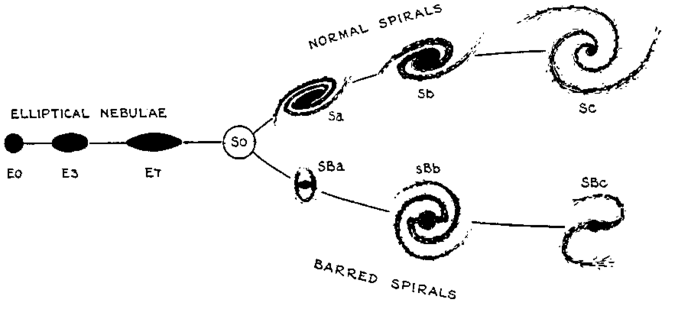
\includegraphics[width=\textwidth]{TuningForkHubble.png}
	\caption{The Hubble tuning-fork diagram. The image is originally from \cite{Hubble1936}.}
	\label{figure:tuning_fork}
\end{figure}

In the Hubble classification, elliptical galaxies are further divided into eight different subcategories according to their observed apparent ellipticity. These categories range from E0 to E7, where the number denotes the ellipticity of the galaxy multiplied by ten and rounded to the nearest integer. The ellipticity of a galaxy is simply the measure of how flattened an observed 2D-projection of a ellipsoidal stellar system is. It can be calculated using the equation:
\begin{equation}
\epsilon = 1 - \frac{b}{a}, \label{eq:ellipticity}
\end{equation}
where $a$ and $b$ are the semi-major and semi-minor axes of a luminosity isophote (i.e. a constant luminosity or surface brightness contour), respectively. The larger the ellipticity, the flatter the system ($\epsilon = 0$ denotes a completely spherical galaxy). It is important to note, however, that the ellipticity of a system depends on the isophote from which it is calculated. Since the isophotes of elliptical galaxies generally become flatter the farther they are located from the galactic centre \citep{BinneyTremaine}, this results in a single galaxy having multiple potential ellipticities. To remedy this, the Hubble classification uses the ellipticity at the effective radius ($R_e$) to determine the subcategory of an elliptical galaxy. The effective radius is the radius of a sphere that encloses half of the total luminosity of the galaxy. Since galaxies do not have clearly defined boundaries, $R_e$ is also often used as a measure of their size. 

\subsection{Photometry} \label{section:ellip_photo}

The photometric properties of elliptical galaxies are often described in terms of the surface brightness, which describes the amount of observed luminosity from a unit area. Thus, an important property for studying the general spatial distribution of stellar material in observed elliptical galaxies, is the one-dimensional radial surface brightness profile $I(R)$, where $R$ is the projected distance from the centre of the galaxy. In practice, these profiles can be constructed from observations by calculating the azimuthal averages of the observed surface brightness at every projected radius $R$ \citep{MerrittBook}.

The observed surface brightness profiles of elliptical galaxies are typically smooth and featureless, declining smoothly as the projected radius grows, until the galaxy is indistinguishable from the background \citep{BinneyTremaine}. These observed "power-law"-like profiles are quite similar in shape across all elliptical galaxies, which has led to the formulation of a multitude of models that attempt to describe this general shape. An early example of such a model is the "de Vaucouleurs" power-law profile: $I \propto R^{1/4}$ \citep{deVaucouleurs1948}. This model, however, is quite simple, and only represents well the profiles of some elliptical galaxies, namely the bright ellipticals \citep{MerrittBook}. 

Compared to the de Vaucoulers-profile, a more robust and more commonly used model is the Sérsic-profile \citep{Sersic1968}:
\begin{equation}
I (R) = I_e \exp \{ -b_n \left[ (R / R_e)^{1/n} \right] \},
\end{equation}
where $R$ is again the projected distance from the galactic centre, $I_e$ is the surface brightness at the effective radius, $n$ is the so-called Sérsic index ($n=4$ gives a Sérsic profile which is identical to the de Vaucouleurs profile), and $b_n$ is a shape factor, which is defined so that a circular area with a radius of $R_e$ contains half of the total luminosity of the galaxy. The value for the shape factor can be approximated as $b_n \approx 2n - 0.324$, when $1 \lesssim n \lesssim 10$ \citep{BinneyTremaine}. 

The prominent use of the Sérsic-profile is due to the fact, that it describes the observed surface brightness profiles of many different elliptical galaxies very well for a large range of radii \citep{MerrittBook}. However, when extrapolated to the central regions of galaxies, the profile often deviates from the observations. The galactic cores either contain "missing" or "extra" light, corresponding to what are often called "cored" or "cuspy" central surface brightness profiles, respectively \citep[e.g.][]{Kormendy2009}.

Whether the central surface brightness profile of an elliptical galaxy is a shallow "cored" profile or a steep "cuspy" profile is seemingly tied to the absolute magnitude of the galaxy. Typically, bright ellipticals ($\mathcal{M_V} \lesssim -22$) have central profiles with missing light, while fainter galaxies ($-22 \lesssim \mathcal{M_V} \lesssim -16$) contain extra light at their centres \citep{Kormendy2009}. 

This supposed dichotomy between the brighter and fainter ellipticals also extends to the isophotal shapes of the galaxies. Usually the shapes of the isophotes of elliptical galaxies deviate from exact ellipses, as the brighter ellipticals contain so-called "boxy" isophotes, while the isophotes of the fainter galaxies are typically more "disky" (an illustration of the two isophotal shapes can be seen in figure \ref{figure:isophotes}) \citep{GalaxyFormationAndEvo2010}. Whether the shapes of the isophotes are "boxy" or "disky", can be determined from the deviations of the observed isophotes from their respective best-fit ellipses. More specifically, this is done using the Fourier-series of the deviations, which is described by the following formula:
\begin{equation}
\Delta (\phi) = R_\mathrm{iso}(\phi) - R_\mathrm{ell}(\phi) = a_0 + \displaystyle\sum^\infty_{n=1} (a_n \cos(n\phi) + b_n \sin(n\phi)), \label{eq:isophote_deviations}
\end{equation}
where $R_\mathrm{iso}(\phi)$ is the radius of the isophote at the angle $\phi$, $R_\mathrm{ell}(\phi)$ is the radius of the corresponding best-fit ellipse at the same angle, and where $a_n$ and $b_n$ are the Fourier coefficients. If $a_4 < 0$ holds true the isophote is considered "boxy", and if $a_4 > 0$ holds true the shape of the isophote is deemed to be "disky".

\begin{figure}
	\centering
	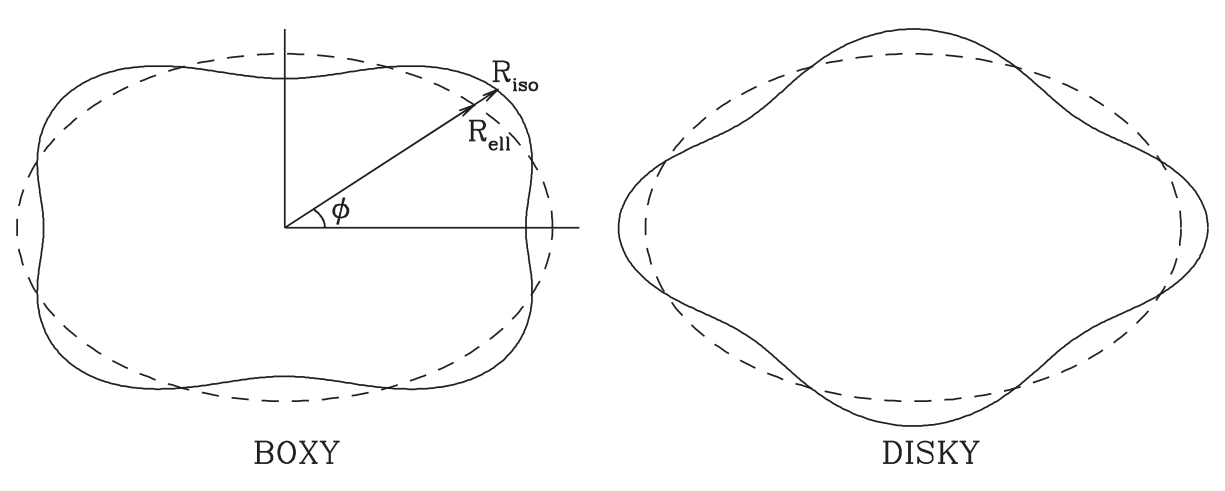
\includegraphics[width=\textwidth]{boxy_and_disky_GFE.png}
	\caption{A comparison between the isophotal shapes of "boxy" and "disky" galaxies. The solid curves denote the respective isophotal shape, while the dashed lines denote their best-fit ellipses. The markings on top of the picture of the "boxy" isophote, illustrate the procedure described by equation \ref{eq:isophote_deviations}. The figure is adopted from from \cite{GalaxyFormationAndEvo2010}.}
	\label{figure:isophotes}
\end{figure}

\subsection{Kinematics} \label{section:ellip_kinematics}

The divide between bright and faint elliptical galaxies, specified in the previous section, seems to extend to the kinematic properties of the galaxies \citep[discussed in e.g.][]{GalaxyFormationAndEvo2010}. The brighter galaxies rotate slowly, while the rotation of the fainter galaxies is faster, with luminosity weighted rotational velocities of $\sim 10 \mathrm{km/s}$ and $\sim 100 \mathrm{km/s}$, respectively \citep{Davies1983, Cappellari2007}. Furthermore, the velocity distributions of the bright "boxy" galaxies are relatively anisotropic, with different degrees of velocity dispersion along their three principal axes and a large amount of random stellar motion compared to the amount of ordered motion. This contrasts with the more isotropic and ordered velocity distributions of the fainter and more disk-like galaxies \citep{Kormendy2009, Krajnovic2008}. How ordered the velocity distribution of a galaxy is, can be seen in the values of its $V/\sigma$-parameter, where $V$ and $\sigma$ are the line-of-sight maximum rotational velocity and the velocity dispersion at the centre of the galaxy, respectively. The value of $V/\sigma$ is generally $\lesssim 0.1$ for the bright galaxies, which is smaller than the value of $V/\sigma \sim 1$ that the fainter galaxies have.

\begin{figure}[h]
	\centering
	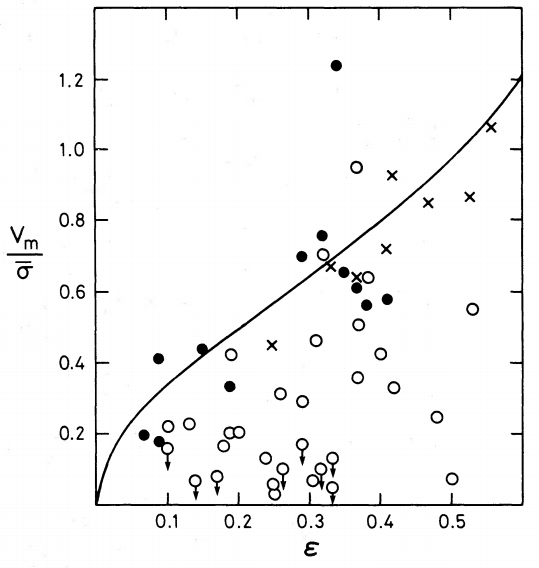
\includegraphics[width=0.60\textwidth]{davies_v-sigma.png}
	\caption{Plot of the $V/\sigma$ – $\epsilon$-relation. The solid curve is defined by equation \ref{eq:v-sigma-epsilon} and shows the expected relation for galaxies with isotropic rotation. The filled circles denote elliptical galaxies with a $B$-band magnitude of $M_B > -20.5$, while the open circles are for galaxies with $M_B < -20.5$. The crosses stand for bulges of disk galaxies. The figure is adopted from \cite{Davies1983}.}
	\label{figure:v-sigma}
\end{figure}

The more ordered and faster rotation of the fainter galaxies, seems to be at least in part consistent with rotational flattening. Rotational flattening occurs in isotropic rotators, for which the value of the $V/\sigma$-parameter is expected to approximately follow the equation:
\begin{equation}
\frac{V}{\overline{\sigma}} \approx \sqrt{\frac{\epsilon}{1-\epsilon}}, \label{eq:v-sigma-epsilon}
\end{equation}
where $\overline{\sigma}$ is the mean velocity dispersion inside half of the effective radius and $\epsilon$ is the ellipticity of the galaxy. This gives a relation between the rotation and the expected ellipticity of the galaxy, often noted as the $V/\sigma$ – $\epsilon$-relation. Figure \ref{figure:v-sigma} shows the $V/\sigma$ – $\epsilon$-relation from \ref{eq:v-sigma-epsilon}, alongside the observed apparent ellipticities and $V/\sigma$-parameters for elliptical galaxies with a $B$-band magnitude of either $M_B > -20.5$ (filled circles) or $M_B < -20.5$ (open circles) \citep{Davies1983}. By looking at the figure, it is clear that when compared to the brighter galaxies, the fainter galaxies are in general situated closer to the curve describing the expected relation. This implies that unlike the boxy bright ellipticals, the disky faint ellipticals are in fact flattened by rotation. The generally weaker flattening of the brighter galaxies is then usually attributed to their anisotropic velocity distributions, since stellar systems are naturally more extended along the axes where their velocity dispersion is larger.

A further distinction between the bright and relatively faint ellipticals can be drawn from their gravitational potentials. The "disky" galaxies are assumed to be axisymmetric, with an ellipsoidal shape containing two identical-length semi-principal axes ($A = B \neq C$). On the other hand, the "boxy" galaxies seem to be triaxial, with all of their semi-principal axes having different lengths ($A \neq B \neq C$) \citep{GalaxyFormationAndEvo2010}. 

The triaxial potential of the bright ellipticals can be identified from the fact that they often contain kinematic misalignments, where the position angle of their 2D projected kinematic axis differs from their photometric minor axis. According to \cite{GalaxyFormationAndEvo2010}, these misalignments can arise as a result of two different effects, both relating to the inclusion of a triaxial potential. Firstly, a kinematic misalignment might be caused by a difference in the directions of the projected and the apparent observed minor axes of the galaxy. This property is common in triaxial galaxies, due to their asymmetric shape. On the other hand, the deviation in the position angles might also be the result of the galaxy having an intrinsically misaligned angular momentum. This is also a natural consequence of triaxial potentials, as they support rotation around all three axes. 

\begin{figure}
	\centering
	\begin{subfigure}[b]{0.49\textwidth}
		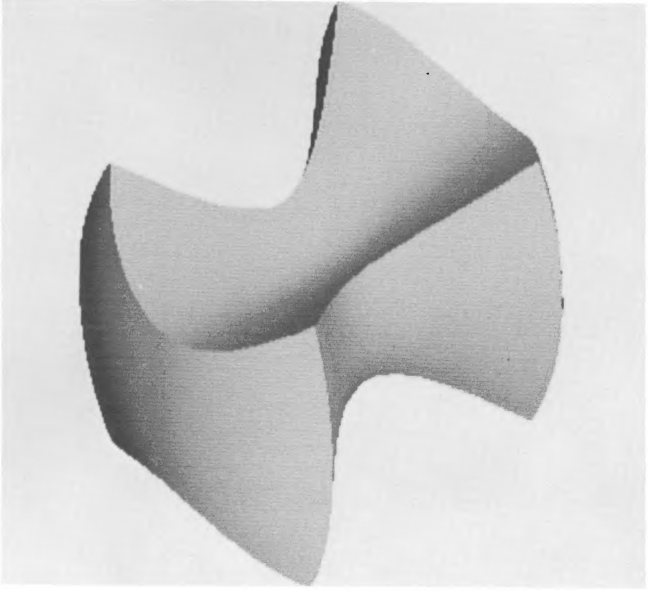
\includegraphics[width=\textwidth]{statler_box.png}
		\caption{Box-orbit}
	\end{subfigure}
	\begin{subfigure}[b]{0.49\textwidth}
		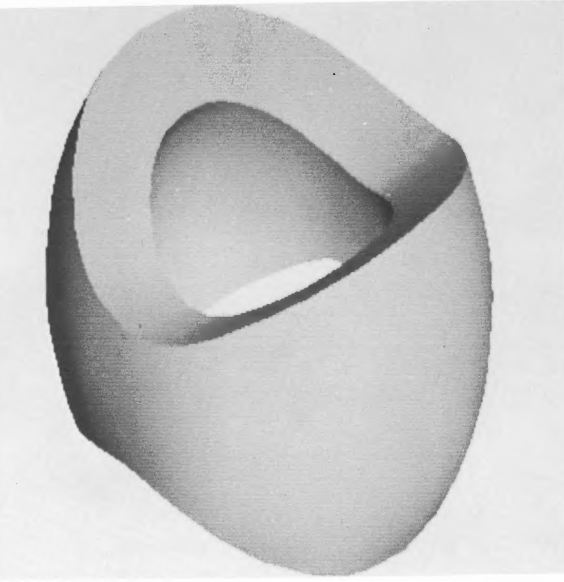
\includegraphics[width=\textwidth]{statler_short_tube.png}
		\caption{Short-axis tube-orbit}
	\end{subfigure}
	\begin{subfigure}[b]{0.49\textwidth}
		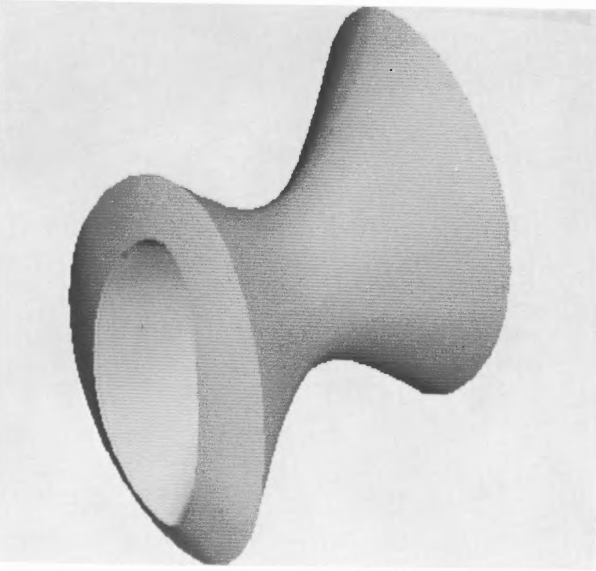
\includegraphics[width=\textwidth]{statler_long_inner.png}
		\caption{Inner long-axis tube-orbit}
	\end{subfigure}
	\begin{subfigure}[b]{0.49\textwidth}
		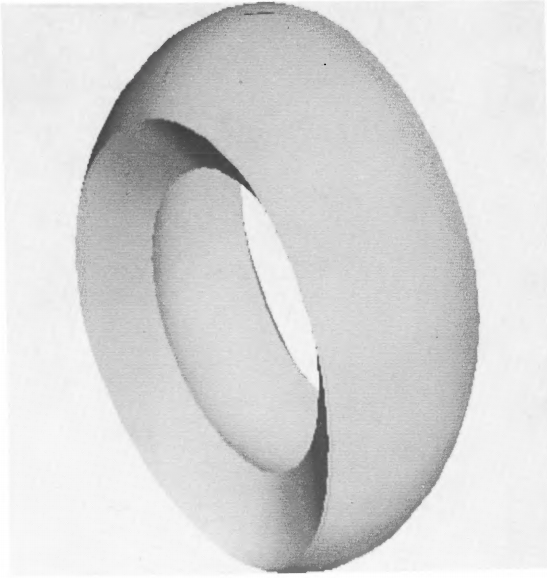
\includegraphics[width=\textwidth]{statler_long_outer.png}
		\caption{Outer long-axis tube-orbit}
	\end{subfigure}
	\caption{Models of different orbital types that can occur in triaxial potentials. The figures are adopted from \cite{Statler1987}.}
	\label{figure:triaxial_orbits}
\end{figure}

Depending on the shape of its gravitational potential, galaxies support different kinds of orbits. The axisymmetric potentials of the "disky" galaxies support both so-called tube-orbits, which trace a ring-like volume around the axis-of-symmetry, and the cone-shaped saucer-orbits \citep{MerrittBook}. Triaxial galaxies, on the other and, support at least four different kind of orbits, models of which can be seen in figure \ref{figure:triaxial_orbits}. Three of these are different types of tube-orbits. They volume that they trace, is located either around the short axis, the inner long axis, or the outer long axis. The fourth orbital type supported by triaxial galaxies is the box-orbit. These orbits fill a rectangular volume, and stars that inhabit them can move through the centre of the galaxy. Box-orbits are often the dominant stellar component in triaxial potential models, giving the "boxy" galaxies their characteristic shape \citep{BinneyTremaine}.

%Slowly rotating bright ellipticals often exhibit so-called \textit{Kinematically Distinct Cores} (KDCs). KDCs are central regions of galaxies with an angular momentum that has a different or even opposite direction when compared to the rest of the galaxy. Once again, the existence of a KDC in a galaxy might point to the host being triaxial, as they could simply be projections of major families of circulating orbits in a triaxial potential \citep{Statler1991, GalaxyFormationAndEvo2010}.% It is also possible, however, that the KDCs have formed from the accretion of other galaxies onto the host galaxy, meaning that they might not be able to be used as markers of triaxial potentials.

\subsection{Formation Models}

There are two main models for the formation of elliptical galaxies: the monolithic collapse scenario and the merger scenario \citep{GalaxyFormationAndEvo2010}. In the monolithic collapse scenario, elliptical galaxies are formed through the collapse and stabilization of some initial condition, which results in the simultaneous formation of the stellar material and the assembly of the galaxy. Depending on whether the initial conditions contain gas, this collapse can either be "dissipative" or "dissipationless". In a dissipative process the system loses some of its total energy through radiation, while in a dissipationless process the total energy is conserved. The inclusion of a gaseous component in the initial condition of the collapse makes it dissipative, as the gas is turned into stars during the collapse. A dissipationless collapse then usually necessitates a lack of gas.

Assuming that the collapse in the monolithic collapse scenario is dissipative, the model in question is able to reproduce several features observed in actual ellipticals, such as a smaller ratio of dark matter to baryonic matter in the centre of the galaxy than in the outer regions \citep{GalaxyFormationAndEvo2010}. However, the main problem of the model is that it is not compatible with the current paradigm that expects a $\Lambda CDM$ cosmology for the universe. 

The cold dark matter (CDM) cosmology assumes a hierarchical formation for observed large-scale structures. It also expects that star formation and the merging of dark matter halos are still on-going processes. This is in stark contrast to the monolithic collapse scenario, where after the initial collapse, the resulting stellar system evolves mostly passively. The galaxy would not experience any major mergers nor star-formation.

The merger scenario suggests that elliptical galaxies are formed through mergers of two or more pre-existing and fully formed galaxies \citep{GalaxyFormationAndEvo2010}. This means that, in its purest form, the merger scenario assumes that star formation and the assembly of the final galaxy don not occur concurrently, and that they are independent and consequent processes. Naturally, this can not be reconciled with the $\Lambda \mathrm{CDM}$ cosmology.

It has also been suggested that elliptical galaxies are formed through a two-phased mechanism that combines both the monolithic collapse and the merger scenarios \citep[e.g.][]{Oser2010}. According to this model, the stellar material in elliptical galaxies is initially (at redshifts $2 \lesssim z \lesssim 6$) accumulated through a process similar to the 'monolithic collapse' scenario, where the stars are formed 'in-situ' by flows of cold gas. Afterwards ($z \lesssim 3$), the elliptical galaxies are expected to grow as a result of both minor and major galaxy mergers (i.e. the accumulated stars are formed 'ex-situ'). 

Taking into account the hierarchical nature of the $\Lambda \mathrm{CDM}$-cosmology, the formation models that include galaxy mergers seem to be the most representative of the actual mechanism from which elliptical galaxies have been formed. Thus, the existence of the observed photometric and kinematic dichotomy between the "core" and "cusp" galaxies, has been interpreted to be the result of differences in their respective merger progenitor galaxies. There are multiple properties that can affect the merger remnant. For example, the ratio between the masses of the galaxy progenitors in a merger, has an effect on the rotational velocity of the remnant \citep{Naab2003}. However, the observed dichotomy is usually attributed to the existence of dissipative components in the merging galaxies \citep{GalaxyFormationAndEvo2010}.

The fainter Es with "cuspy" central surface brightness profiles, are generally thought to have been formed through dissipative mergers of gas-rich progenitor galaxies. Driven by tidal perturbations during the merger, this gas is expected to accumulate in the centre of the merger remnant, resulting in a starburst event \citep{Barnes1991}. This sudden increase in the central stellar density, would account for the extra-light seen in the surface brightness profiles of the faint galaxies \citep{Hopkins2008}, and would deepen the central gravitational potential well, causing the velocity dispersion in the core regions of the remnant galaxy to rise \citep{Barnes1996}. The stronger central gravitational potential would also cause the gravitational potential of the whole galaxy to become more axisymmetric. As box-orbits can only occur in triaxial-potentials, this would result in the remnant becoming more disk-like in shape, which is a characteristic appearance for the fainter galaxies \citep{Naab2006}.

In contrast, the formation mechanism for the "core" galaxies is that of a dissipationless "dry" merger. The formation of massive slowly rotating galaxies is assumed to be a two-stage process, similar to the model proposed by \cite{Oser2010}. Initially, the accumulation of stellar mass in "core" galaxies is driven by rapid "in-situ" star formation caused by inflows of cold gas. Afterwards, during redshift $3 > z > 0$, their growth in mass is dominated by major gas-poor ETG mergers \citep{Naab2009}. Since the massive galaxies in major galaxy mergers are expected to contain central supermassive black holes (SMBHs), it is often proposed that the "cores" in the bright ellipticals are a result of a scouring process, where the central binary black hole coalesces and ejects stellar material from the centre of the merger remnant in complex three-body interactions.

\section{Core Galaxies} \label{section:core_galaxies}

While the basic principle of core galaxies being galaxies with "missing" light at their centre is easy to grasp, giving an explicit definition for what exactly constitutes a core galaxy is somewhat more challenging. One definition given for core galaxies, is that they are galaxies with an observed surface brightness profile defined similarly to equation \ref{eq:nuker}, where the inner logarithmic slope has a value of $\gamma < 0.3$ \citep{Lauer1995, Lauer2007}. However this definition is problematic, as galaxies that do not contain a central light deficit but have a low value for the Sérsic index $n$, can also have shallow inner profiles \citep{Graham2003}. Thus, a simplified definition proposed by \cite{Kormendy1999}, describes core galaxies as galaxies with a surface brightness profile that is a combination of two different profiles. These being a shallow inner profile and a steep outer power-law profile. This definition is also questionable however, since it results in a disconnection with the curved outer Sérsic profiles that are known to exist \citep{Dullo2012}. \cite{Graham2003} then suggest that, core galaxies should simply be defined through the light deficit in their observed central surface brightness profile. This deficit can be identified by comparing the observed profile to the inward extrapolation of the outer Sérsic profile.

The size of the core is an important property of core galaxies. Its relation to the other properties observed in the galaxy, can be used to derive information about the formation history of both the galaxy itself and the low-luminosity core. Usually the core-size is determined by fitting observed surface brightness profiles with some model profile that combines a shallow inner profile and a steep outer profile. The radius at which the outer profile changes into the the inner profile is called the break radius ($r_b$), and is commonly equated to the radius of the core.

There are two frequently used options for modelling the surface brightness profiles. The first one is the core-Sérsic profile \citep{Graham2003}, which can be expressed using the following equation:
\begin{equation}
\mu(r) = \mu' \left[ 1 + \left( \frac{r_b}{r} \right)^\alpha \right]^{\gamma / \alpha} \exp \left\lbrace -b_n \left[ \left( r^\alpha + r_b^\alpha \right) / r_e^\alpha \right]^{1/(\alpha n)} \right\rbrace, \label{eq:core-sersic}
\end{equation}
where $r_b$ is the break radius, $\gamma$ is the logarithmic slope of the inner power-law profile, $\alpha$ controls the sharpness of the transition between the two profiles, $b_n$, $r_e$ and $n$ are the shape factor, effective half-mass radius and the Sérsic index of the outer Sérsic profile respectively, and the normalization factor $\mu'$ is defined by:
\begin{equation}
\mu' = \mu_b 2^{-\gamma/\alpha} \exp \left[ b_n \left( 2^{(1/\alpha)} r_b/r_e \right)^{1/n} \right], 
\label{eq:mu_dot}
\end{equation}
where $\mu_b$ is the surface brightness at the break radius. 

The second option is to use the so called Nuker profile, a combination of two power-laws \citep{Lauer1995}. The Nuker profile can be written as follows:
\begin{equation}
\mu(r) = 2^{(\beta - \gamma) / \alpha} \mu_b \left( \frac{r_b}{r} \right)^\gamma \left[ 1 + \left( \frac{r}{r_b} \right)^\alpha \right]^{(\gamma - \beta)/\alpha},
\label{eq:nuker}
\end{equation}
where $r_b$ is once again the break radius, $\mu_b$ is the surface brightness at the break radius, $\beta$ and $\gamma$ are the logarithmic slopes of the power-laws inside and outside of the break radius respectively, and $\alpha$ once again describes the sharpness of the transition between the two slopes.

In addition to the model fitting methods, one could also estimate the size of the core by calculating the so-called "cusp radius" $r_\gamma$. The cusp radius is the distance from the centre of the galaxy, at which the logarithmic slope of the surface brightness profile equals $\gamma' = -1/2$ \citep{Carollo1997, Lauer2007Cusp}. This distance provides an estimate for the location where the inner power-law profile changes into the outer profile. Thus, $r_\gamma$ can be equated to the core radius. 

\section{Core Formation Through Black Hole Mergers}

As stated before, currently the leading mechanism for the formation of the cores seen in massive ETGs, is the ejection of stellar material due to three-body interactions between stars and a binary supermassive black hole during an ETG merger \citep[e.g.][]{Faber1997, Milosavljevic2002, GalaxyFormationAndEvo2010}. Core formation is expected to occur specifically during "dry" ETG mergers, as due to the lack of gas, they do not contain merger induced star-formation. A star-burst event occuring during the merger, could mask the formation of the low-luminosity core.

There are three different, and potentially overlapping, phases for SMBH mergers: the dynamical friction phase, the three-body interaction phase, and the gravitational wave radiation phase \citep{MerrittBook}. In each of the three phases, a different process removes kinetic energy and shrinks the separation between the coalescing SMBHs.

\subsection{Dynamical Friction}

During the dynamical friction phase, the relative orbits of the central SMBHs of the merging galaxies, shrink due to changes in their kinetic energies, caused by so-called dynamical friction. Originally proposed by \cite{Chandrasekhar1943}, it is argued that stars experience a net decelerating gravitational force when moving through a population of field-stars. As the subject star moves through the stellar population, its gravitational influence causes the relative trajectories of nearby field-stars to curve behind it. This causes the concentration of mass to become larger behind the subject star than in front of it. The distribution of mass relative to the subject star becomes asymmetric, causing the gravitational force opposite to its direction of motion, to become stronger than the gravitational force parallel to the motion. Thus the star experiences a net decelerating force, also called dynamical friction. A sketch of this mechanism can be seen in figure \ref{figure:dynamical_friction}. Important to note is that, while dynamical friction has so-far only been discussed as being caused by stars, other baryonic matter as well as dark matter, also contribute to its strength.

Dynamical friction also applies to the central SMBHs in galaxy mergers, as they move through the stellar population and the dark matter halo of the galaxy merging with their host. Dynamical friction is initially the main mechanism which shrinks the orbits of the SMBHs, causing them to sink into the centre of the galaxy merger. The strength of the dynamical friction force induced onto the individual SMBHs, can be described by the following equation \citep{BinneyTremaine}:
\begin{equation}
F_\mathrm{DF} = M\frac{d\mathbf{v_\bullet}}{dt} = -4\pi G^2 M^2 m \ln \Lambda \int d^3 \mathbf{v}_a f(\mathbf{v}_a) \frac{\mathbf{v_\bullet}-\mathbf{v}_a}{|\mathbf{v_\bullet}-\mathbf{v}_a|^3,} \label{eq:dynamical_friction}
\end{equation}
where $M$ and $\mathbf{v_\bullet}$ are the mass and velocity of the SMBH, respectively; $m$ and $\mathbf{v_a}$ are the mass and velocity of a field-particle; $f\left(\mathbf{v}_a\right)$ is the phase space density (see section \ref{section:collisionless}) of the field-particles; and $\ln \Lambda$ is described by the equation $\ln \Lambda \simeq \ln \left( \frac{b_\mathrm{max}}{b_{90}} \right)$, with $b_\mathrm{max}$ and $b_{90}$ being the maximum length and the $90^\circ$ reflection impact parameters, respectively.

As can be seen from equation \ref{eq:dynamical_friction}, the strength of the dynamical friction force scales with the mass of the SMBH as $F_\mathrm{DF} \propto M^2$. This shows that, the time it takes for an object to fall to the centre of a stellar system as a result of a dynamical friction driven inspiral, is dependent on the mass of said object. Thus in galaxy mergers, only objects that have a large enough mass, such as SMBHs, can fall to the centre of the merger, and consequently form cores through three-body interactions. This can be seen in for example globular clusters, which are old gas-free stellar systems with masses of $M \sim 10^5 M_\odot$ \citep{BinneyTremaine}. They can still be seen orbiting around the nucleus of the Milky Way, implying that despite their relatively large mass, the time-scale for their inspiral is longer than the age of the Milky Way.

\begin{figure}
	\centering
	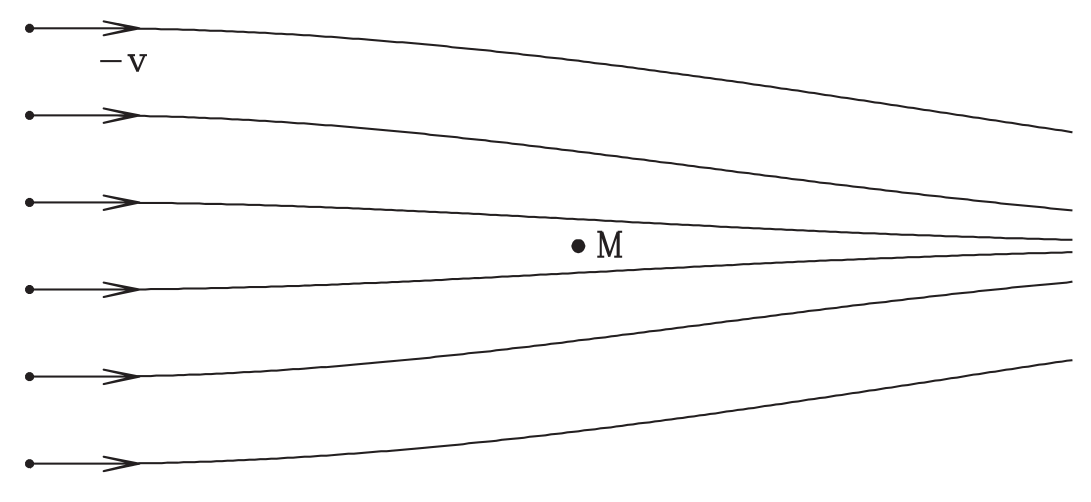
\includegraphics[width=0.8\textwidth]{mo_dynamical_friction.png}
	\caption{A graphical depiction of dynamical friction. The point denoted as $M$ depicts the object moving through the population of field-stars. The smaller dots and the lines are the field-stars and their trajectories, respectively. The arrows show the velocity ($-v$) of the stars in relation to the mass $M$. The figure is adopted from \cite{GalaxyFormationAndEvo2010}.}
	\label{figure:dynamical_friction}
\end{figure}

The effects of dynamical friction continue until the black holes form a so-called "hard binary". A hard binary is a binary system with a binding energy that is larger, than the kinetic energy of the field stars \citep{BinneyTremaine}. The formation of a hard binary occurs, when the relative velocities of the black holes in the binary become much larger, than the velocity dispersion of the surrounding stars. This, in turn, occurs when the coalescing black holes reach a separation of:
\begin{equation}
a = \frac{G\mu}{4\sigma},
\end{equation}
where $\sigma$ is the velocity dispersion of the surrounding stars, and $\mu$ is the reduced mass of the binary, defined using the masses $M_1$ and $M_2$ of the black holes as: $\mu = M_1M_2 / M_1 + M_2$ \citep{MerrittBook}.

\subsection{Three-Body Interactions} \label{section:three-body}

The three-body interaction phase of the SMBH merger, is the phase that is assumed to cause the actual formation of the core. In this phase, the removal of the orbital energy and the shrinking of the orbit, are caused by complex three-body interactions between the binary and surrounding stars. The phase in question usually starts before the formation of the hard binary, at the point when the smaller SMBH falls inside the gravitational sphere-of-influence (SOI) of the more massive black hole \citep{MerrittBook}. At this point the SMBHs can be considered to form a binary. 

The SOI of an SMBH is the spherical region in space, where the gravitational force of the SMBH dominates over the force of the surrounding stars. It encompasses an amount of stellar mass, equivalent to the mass of the black hole. If the velocity dispersion ($\sigma$) of the stars near an SMBH is known, the radius of the spherical region can be determined, by comparing the $\sigma$ to the velocity of a particle on a circular orbit around the SMBH. The following formula describes the length of the so-called influence radius \citep{MerrittBook}:
\begin{equation}
r_\mathrm{SOI} \equiv \frac{GM_\bullet}{\sigma^2} \approx 10.8 \left( \frac{M_\bullet}{10^8 M_\odot} \right) \left( \frac{\sigma}{200 \; \mathrm{km \; s^{-1}}} \right)^{-2} \mathrm{pc},
\end{equation}
where $G$ is the gravitational constant, and $M_\bullet$ is the mass of the black hole. 

As stated before, the orbital energy of the binary is reduced through strong interactions between the binary and surrounding field-stars. Certain stars are able to interact strongly with the SMBH binary, increasing their kinetic energy, causing them to be ejected at high speeds in a "gravitational slingshot" event. This growth in the kinetic energy of the ejected stars, happens at the expense of the orbital energy of the SMBH binary, causing the orbit of the binary to shrink. Whether a star can interact strongly with the SMBH binary, is determined by its relation to the loss-cone. The loss-cone is a region in phase space (see the \textit{Galactic Dynamics} section for the explanation of phase space), where the angular momentum of a star fulfils the following condition:
\begin{equation}
L \lesssim \left[ G(M_1 + M_2) a \right]^{1/2}, \label{eq:loss-cone}
\end{equation}
where $M_1$ and $M_2$ are the masses of the black holes in the SMBH binary, and $a$ is the semi-major axis of the binary orbit \citep{BinneyTremaine}. Only stars that are located inside the loss-cone, can interact strongly with the binary.

\subsection{Gravitational Radiation} \label{section:gravitational_radiation}

Once the three-body interactions with field-stars have shrunk the orbit of the binary enough, gravitational radiation in the form of gravitational waves becomes a significant factor in the evolution of the binary, marking the start of the gravitational wave radiation phase. This occurs when the separation of the SMBHs has become less than:
\begin{equation}
a = \left\lbrace \frac{64}{5} \frac{G^3M_1M_2(M_1+M_2)F(e)}{c^5} \right\rbrace^{1/4},
\end{equation}
where $G$ is the gravitational constant, $M_1$ and $M_2$ are the masses of the black holes, $c$ is the speed of light, and $F(e)$ is an eccentricity-dependent factor.

The orbital energy of the binary is radiated away in the form of gravitational waves, causing the semi-major axis of the binary orbit to become smaller. Interestingly, this also causes the eccentricity of the binary orbit to start to converge at $0$. This effect, is the result of the asymmetry in the decrease of the kinetic energy of the binary, between the pericentre and the apocentre of the orbit. Due to its dependence on the acceleration of the object, the strength of the gravitational radiation is largest when the separation between the SMBHs is at its smallest, meaning that the most significant reduction to the kinetic energies of the black holes occurs near the pericentre of the binary orbit. This circularising effect on the orbit, is analogous to the procedure used to reduce the eccentricity of the orbits of satellites. The velocity of the satellite is decelerated near the pericentre. Due to this deceleration, the satellite is unable to climb as far out in the gravitational well of the central body as it used to. Thus, the central body and the apocentre of the orbit is reduced, resulting in a smaller eccentricity.

An approximation of the rates at which the semi-major axis and the eccentricity of the binary orbit change, can be determined using so-called post-Newtonian dynamics (post-Newtonian dynamics is discussed in greater detail in section \ref{section:PN}). The following equations show these changes averaged over the orbital period, when taking into account PN-terms valid at 2.5PN \citep{Peters1964}:
\begin{equation}
\left\langle \frac{da}{dt} \right\rangle = -\frac{64}{5}\frac{G^3M_1M_2(M_1+M_2)}{c^5a^3(1-e^2)^{7/2}} \left( 1+\frac{73}{24}e^2+\frac{37}{96}e^4 \right), \label{eq:pn_dadt}
\end{equation}
and:
\begin{equation}
\left\langle \frac{de}{dt} \right\rangle = -\frac{304}{15}e\frac{G^3M_1M_2(M_1+M_2)}{c^5a^4(1-e^2)^{5/2}} \left( 1+\frac{121}{304}e^2 \right), \label{eq:pn_dedt}
\end{equation}
for the semi-major axis and the eccentricity, respectively. 

Once enough gravitational energy has been radiated, and the orbit of the black holes has shrunk sufficiently, the SMBHs merge, forming a single black hole. The time it takes for gravitational radiation to cause the coalescence of an SMBH binary, can be calculated using the following equation \citep{MerrittBook}:
\begin{equation}
t_\mathrm{gr} \approx 6 \times 10^6 \frac{(1+q)^2}{q} \; \left( \frac{a}{0.01 \; \mathrm{pc}} \right)^4 \left( \frac{M_1 + M_2}{10^8 M_\odot} \right)^{-3} (1-e^2)^{7/2} \; \mathrm{yr}, \label{eq:t_gr}
\end{equation}
where $q \equiv M_2/M_1 \leq 1$. As equation \ref{eq:t_gr} shows, the efficiency of the final SMBH merger phase depends heavily on the separation between the black holes in the binary ($t_\mathrm{gr} \propto a^4$), as well as the eccentricity of the binary orbit ($t_\mathrm{gr} \propto (1-e^2)^{7/2}$).

\subsection{The Final-Parsec Problem}

The fact that the gravitational radiation driven coalescence is effective only at very small binary SMBH separations, could provide a problem for the existence of actual SMBH mergers. When the SMBH binaries form at the centres of the galaxies their separation is usually $\sim 1 \; \mathrm{pc}$. As equation \ref{eq:t_gr} shows, assuming that the SMBH masses are $\sim 10^8 M_\odot$, and that the binary orbit is circular ($e = 0$, which is admittedly unrealistic, as the SMBH merger orbits are highly elliptical during most of the merger), the black holes would coalesce in a time-scale far longer than the age of the Universe (the age of the Universe is $\sim 13.4 \; \mathrm{Gyr}$). Whether three-body interactions can sufficiently decrease the initial binary separation in order for the gravitational radiation driven coalescence to become efficient, is not certain. As seen in equation \ref{eq:loss-cone}, the size of the loss-cone shrinks as the orbit of the binary becomes smaller. This leads to the problem where, both due to its shrinking size and the ejection of mass from the loss-cone, the number of stars that can interact strongly with the binary becomes so small, that the three-body interaction driven coalescence of the SMBHs effectively ceases. This is called "the final parsec problem" \citep{Milosavljevic2003}.

Several mechanisms, which attempt to reconcile the "final parsec problem" by "repopulating" the loss-cone, have been proposed. These work by supplying the loss-cone with additional stars that can be ejected, further shrinking the orbit of the binary. One such mechanism, is the repopulation of the loss-cone as result of two-body relaxation (see section \ref{section:collisionless}). However, this process has been found to be too inefficient. In nearly all observed galaxies, the relaxation time-scales inside the SOI of the central SMBHs seem to be $\sim 10^{11} \; \mathrm{yr}$ , which is larger than the Hubble time ($\sim 14 \; \mathrm{Gyr}$; \citealt{Faber1997, Milosavljevic2001}). Another proposed repopulation mechanism is the secondary slingshot. In this mechanism, the ejected star experiences too interactions with the SMBH binary, effectively decreasing its energy twice. The initial interaction between the binary and an orbiting star only moves the star into another bound orbit, from which it may interact with the binary once more \citep{MerrittBook}. It is also possible, that the triaxial geometry of massive elliptical galaxies could account for the repopulation of the loss-cone. Torques resulting from the non-spherical gravitational potential in triaxial galaxies can change the angular momentum of stars, potentially causing some stars outside of the loss-cone to be included in the loss-cone regime \citep{MerrittBook, Gualandris2017}. Through simulations, \cite{Gualandris2017} have shown that this "collisionless orbit diffusion", can account for the repopulation of the loss-cone. They even conclude that: "there is no 'final parsec problem'".

\subsection{Observational Evidence for Core Formation Through SMBH Mergers}

Whether the cores of the galaxies actually form through black hole mergers, depends on how probable the occurrence of these kind of events is. The observed empirical relation between the mass of a central SMBH and the velocity dispersion of its host galaxy (see equation \ref{eq:m-sigma}), has shown that all massive galaxies have supermassive black holes in their centres. Thus, a merger of two massive galaxies would undoubtedly contain two SMBHs. 

There have also been some direct observational evidence for SMBH binaries occurring in the centres of galaxies. For example, \cite{Rodriguez2006} observed two active galactic nuclei (AGN) with a projected separation of $\sim 7.3 \; \mathrm{pc}$ in the galaxy NGC 6240. Since AGN are powered by accretion of material onto supermassive black holes, and since the total mass of these supposed BHs in NGC 6240 is $\sim 1.5 \times 10^8 M_\odot$, both of the AGN are inside the gravitational influence radius of the other, and the SMBHs would thus be considered to be a binary. The presence of an SMBH binary has also been observed in the active galaxy OJ 287, where the periodical optical variety of the AGN has been attributed to a smaller SMBH passing through the accretion disk of the larger active black hole \citep{MerrittBook}.

As for the existence of black hole mergers, recent gravitational wave observations performed using the \textit{Laser Interferometer Gravitational-Wave Observatory} (LIGO, \citealt{Abbott2016, Abbott2019}), provide unequivocal evidence that at least stellar-mass black hole mergers can occur. Though SMBH mergers have yet to be observed, the fact that black hole mergers have been shown to exist, alongside the aforementioned binary SMBH observations, greatly supports the idea that merging supermassive black holes could play a part in the evolution of some galaxies. Furthermore, taking into account the fact that our current cosmological paradigm expects galaxies to have been formed through hierarchical mergers of other galaxies, and that all merger progenitor galaxies most likely already contain a central SMBH, it stands to reason that binary SMBHs should exist at some point in most galaxies. Thus, the rarity of binary SMBH observations implies that many of these binary SMBHs have already merged, further suggesting that SMBH mergers are taking place.

\subsection{Black Hole Scaling Relations} \label{section:scaling_relation}

\begin{figure}
	\centering
	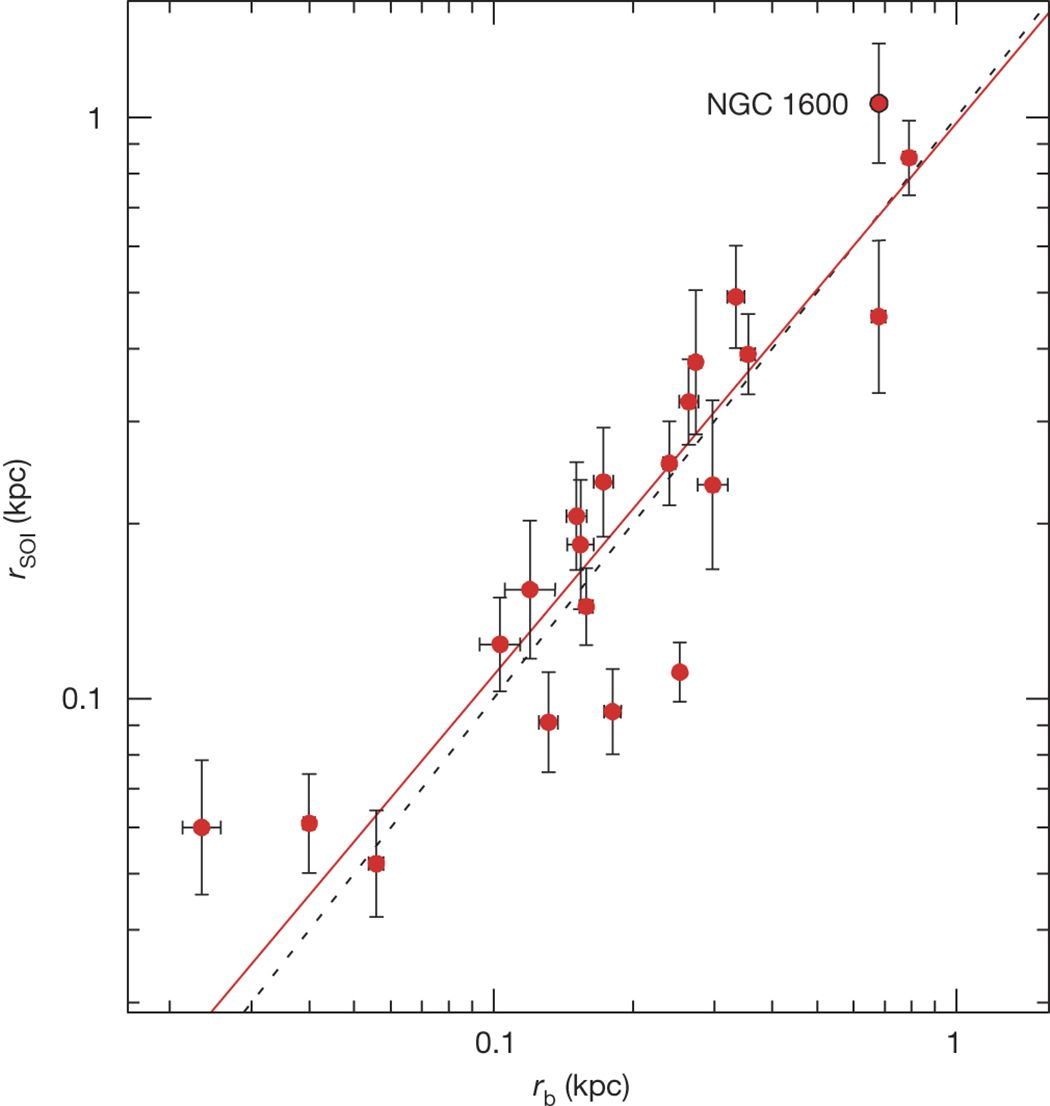
\includegraphics[width=0.7\textwidth]{thomas_mbh-rb.png}
	\caption{Plots of the $M_\bullet$ – $r_b$ relation from equation \ref{eq:m-rb}, alongside the observed data from which the relation has been deduced. The original figure is from \cite{Thomas2016}.}
	\label{figure:m-rb}
\end{figure}

The observed sizes of low-luminosity cores have been found to correlate with the mass of the central SMBH of the galaxy. Both simulations and observations have shown that a relation between the central SMBH mass ($M_\bullet$) and the quantity of the observed mass deficit ($M_\mathrm{def}$) exists \citep{Graham2004, Merritt2006, Dullo2014}. Furthermore, there seems to be a relation between the mass of the SMBH and the radius of the depleted core. \cite{Thomas2016}, for example, derive the following scaling relation from observed core sizes and central black hole mass measurements:
\begin{equation}
\log_{10} \left( \frac{M_\bullet}{M_\odot} \right) = (1.17 \pm 0.14) \log_{10} \left( \frac{r_b}{\mathrm{kpc}} \right) + (10.27 \pm 0.51). \label{eq:m-rb}
\end{equation}
Figure \ref{figure:m-rb} shows this relation alongside observed values for the core radius and the corresponding central black hole mass. While there seems to be quite a bit of scatter between the modelled relation and the observed values, the mass of the central SMBH seems to be connected to the properties of the core. Furthermore, similar relations have been observed by, for example, \cite{Dullo2012}.

\begin{figure}
	\centering
	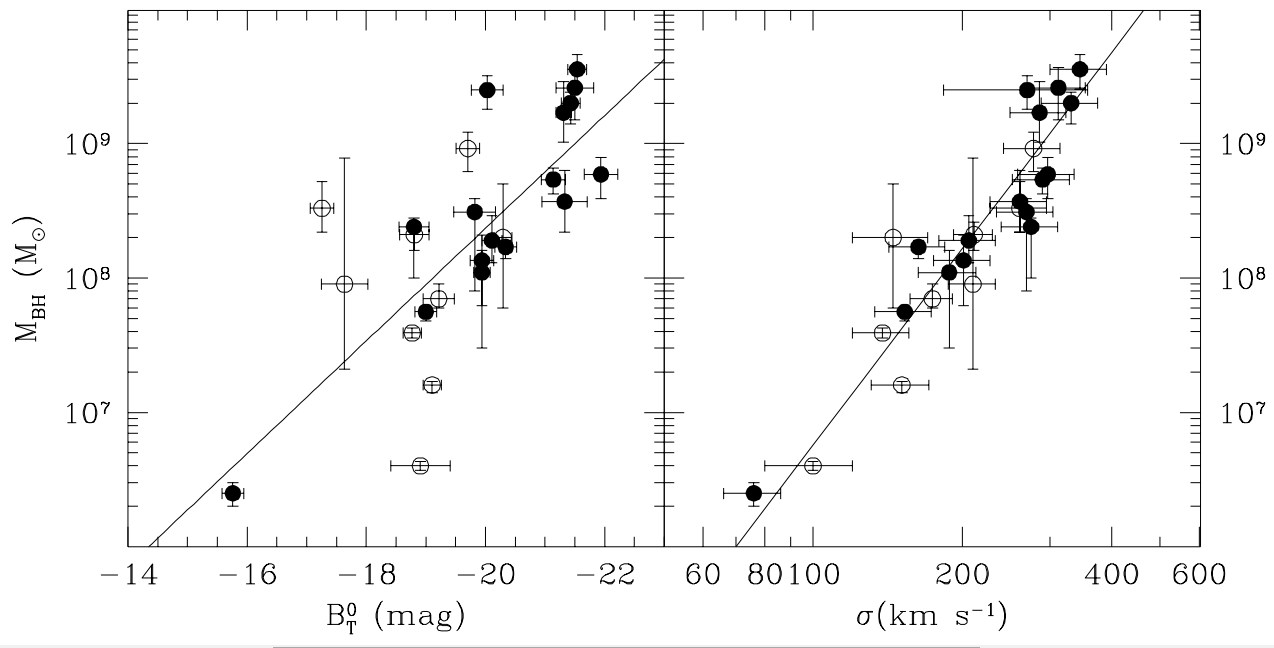
\includegraphics[width=\textwidth]{ferrarese_m-sigma.png}
	\caption{Plots of both the $M_\bullet$ – $L_\mathrm{B,bulge}$ (left) and $M_\bullet$ – $\sigma$ (right) relations, as given by \cite{Ferrarese2005}. The luminosity is given in B-magnitudes in the plot of the $M_\bullet$ – $L_\mathrm{B,bulge}$ relation, and the relation itself differs somewhat from the one described in equation \ref{eq:m-l_bulge}. The open circles denote observations from the bulges of spiral galaxies, and the filled circles denote observations from elliptical galaxies. The figures are originally from \cite{Ferrarese2005}.}
	\label{figure:m-sigma}
\end{figure}

Though not necessarily proving that the formation of the central SMBH is connected to the development of the core; further evidence that the central black hole is inherently linked to the properties of its host galaxy, can be seen in the three main scaling relations of the SMBH mass. The first is the $M_\bullet - \sigma$ relation \citep{Ferrarese2005}:
\begin{equation}
\frac{M_\bullet}{10^8 \; M_\odot} = (1.66 \pm 0.24) \left( \frac{\sigma}{200 \; \mathrm{km \, s^{-1}}} \right)^{(4.86\pm0.43)}, \label{eq:m-sigma}
\end{equation}
where $\sigma$ is the velocity dispersion. The second relation is the $M_\bullet - L_\mathrm{bulge}$ relation \citep{Marconi2003}:
\begin{equation}
\log_{10} \left( \frac{M_\bullet}{M_\odot} \right) = (1.13 \pm 0.12) \log_{10} \left( \frac{L_\mathrm{K,bulge}}{L_\mathrm{K,\odot}} \right) + (8.21 \pm 0.07), \label{eq:m-l_bulge}
\end{equation}
where $L_\mathrm{K,bulge}$ is the luminosity of the galactic bulge in $K$-band magnitudes. Finally, the third relation is the $M_\bullet - M_\mathrm{bulge}$ relation \citep{Marconi2003}:
\begin{equation}
\log_{10} \left( \frac{M_\bullet}{M_\odot} \right) = (0.96 \pm 0.07) \log_{10} \left( \frac{M_\mathrm{bulge}}{M_\odot} \right) + (8.28 \pm 0.06), \label{eq:m-m_bulge}
\end{equation}
where $M_\mathrm{bulge}$ is the mass of the central bulge. Plots for these three relations can be seen in figures \ref{figure:m-sigma} and \ref{figure:m-bulge}. 

The above relations are often explained to be the result of feedback-effects caused by the growth of the central SMBH. Thus, they been used as evidence for the coevolution of the central black holes and their host galaxy. SMBHs are expected to gather most of their mass through the accretion of gas \citep{Soltan1982}, which causes the aforementioned feedback-effects. These effects can be radiative or kinetic, and occur in the form of radiation from the accretion disk and outflows formed from the accreted material, respectively. The strength of the feedback is dependent on the gas accretion rate, and as a consequence, the mass of the accreting black hole. If the SMBH is massive enough, the energy released through the feedback-effects can overcome the galactic bulge binding energy ($E_\mathrm{bulge} \approx M_\mathrm{bulge} \; \sigma^2$; e.g. \citealt{Fabian2012}), sweeping away the interstellar gas from the bulge, thus effectively stopping star formation and further mass accretion by the black hole. Since the binding energy of the bulge is dependent on its mass and velocity dispersion, it is thus strongly implied that this kind of a self-regulating process could result in the $M_\bullet$ – $\sigma$ and $M_\bullet$ – $M_\mathrm{bulge}$ relations. The $M_\bullet$ – $L_\mathrm{bulge}$ relation would then naturally arise as a consequence of the bulge-mass relation.

\begin{figure}
	\centering
	\begin{subfigure}[b]{0.49\textwidth}
		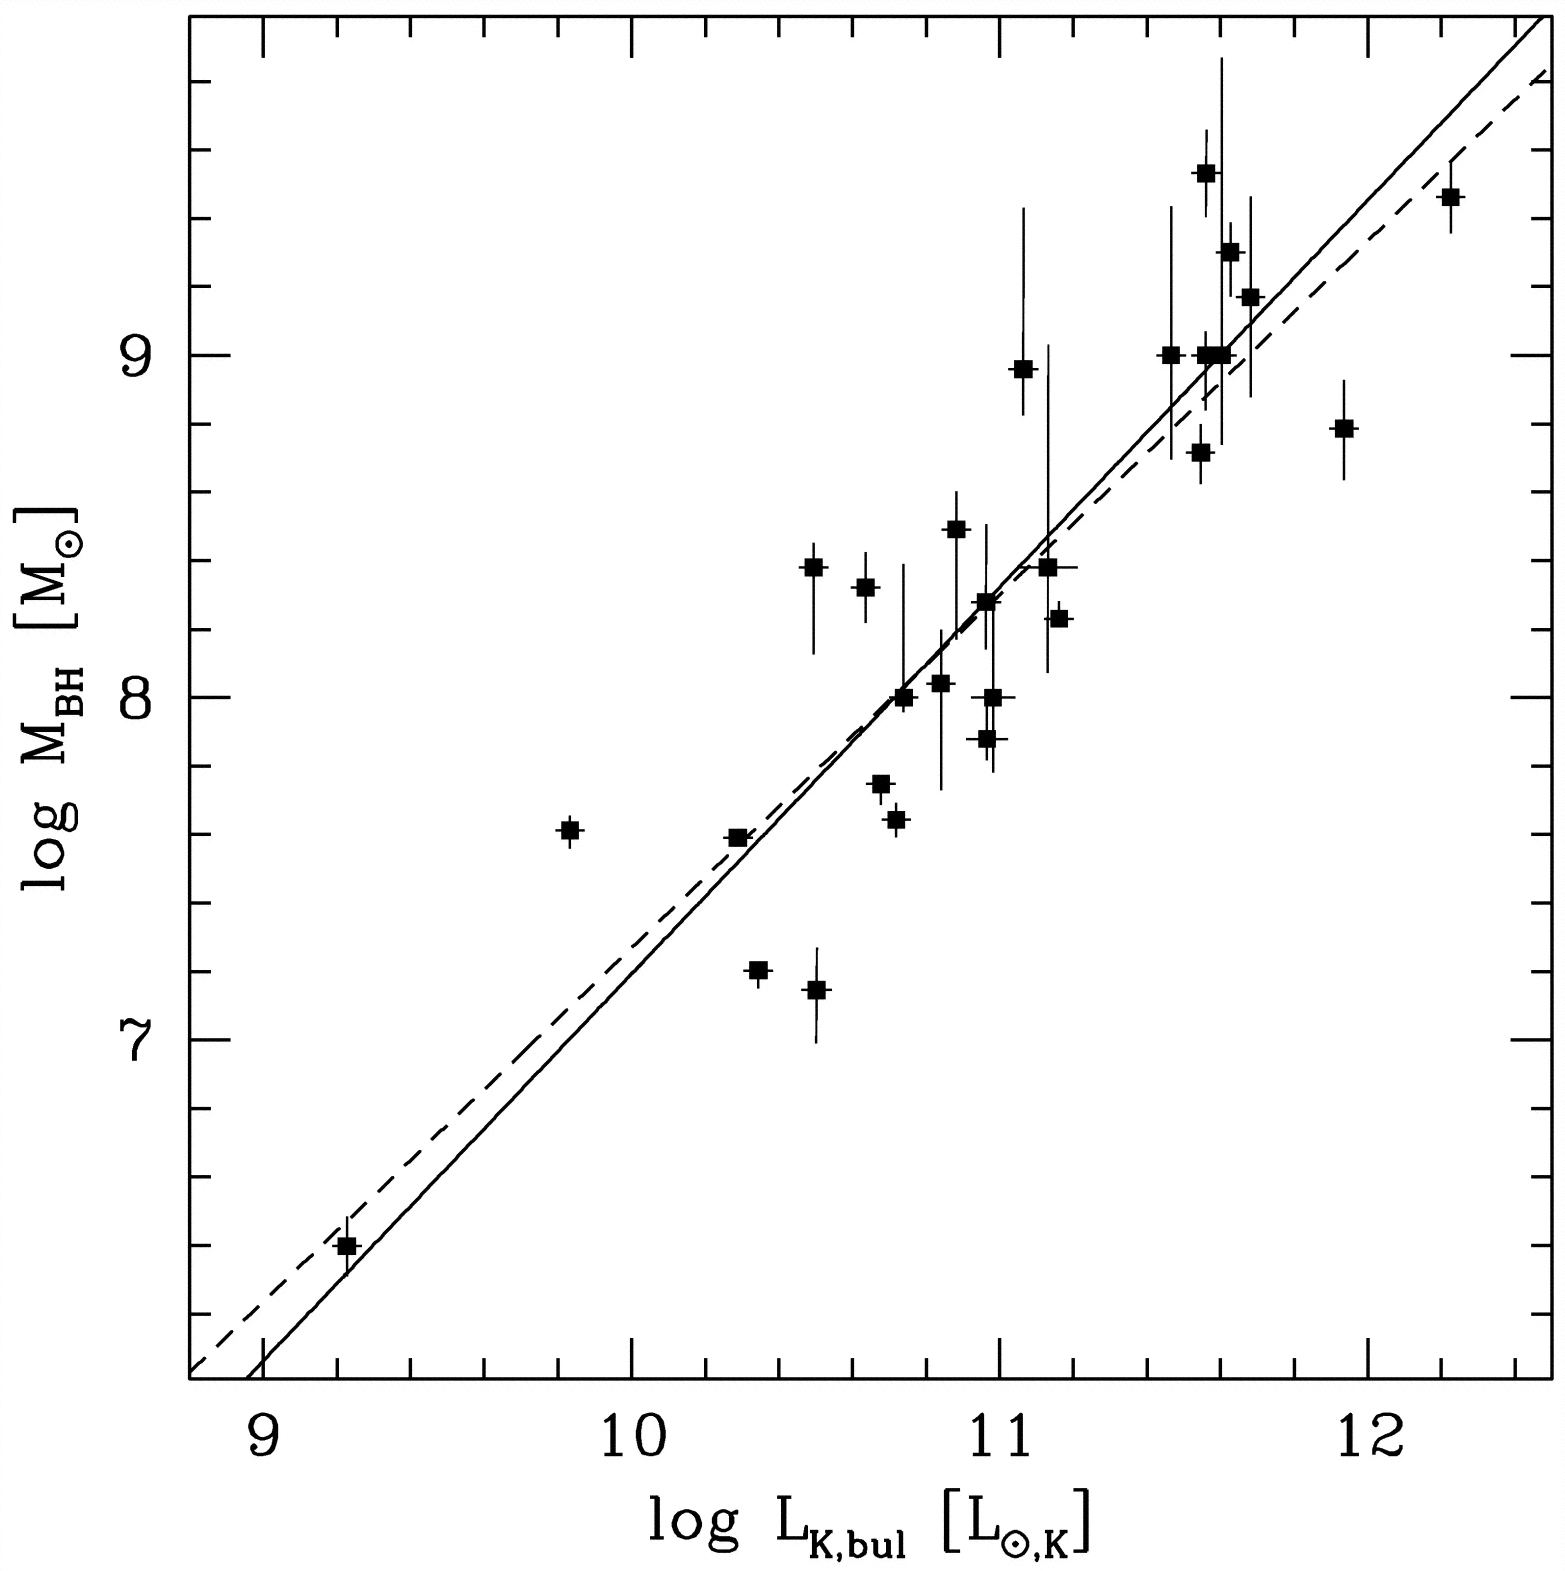
\includegraphics[width=\textwidth]{marconi_l-bul.png}
	\end{subfigure}
	\begin{subfigure}[b]{0.49\textwidth}
		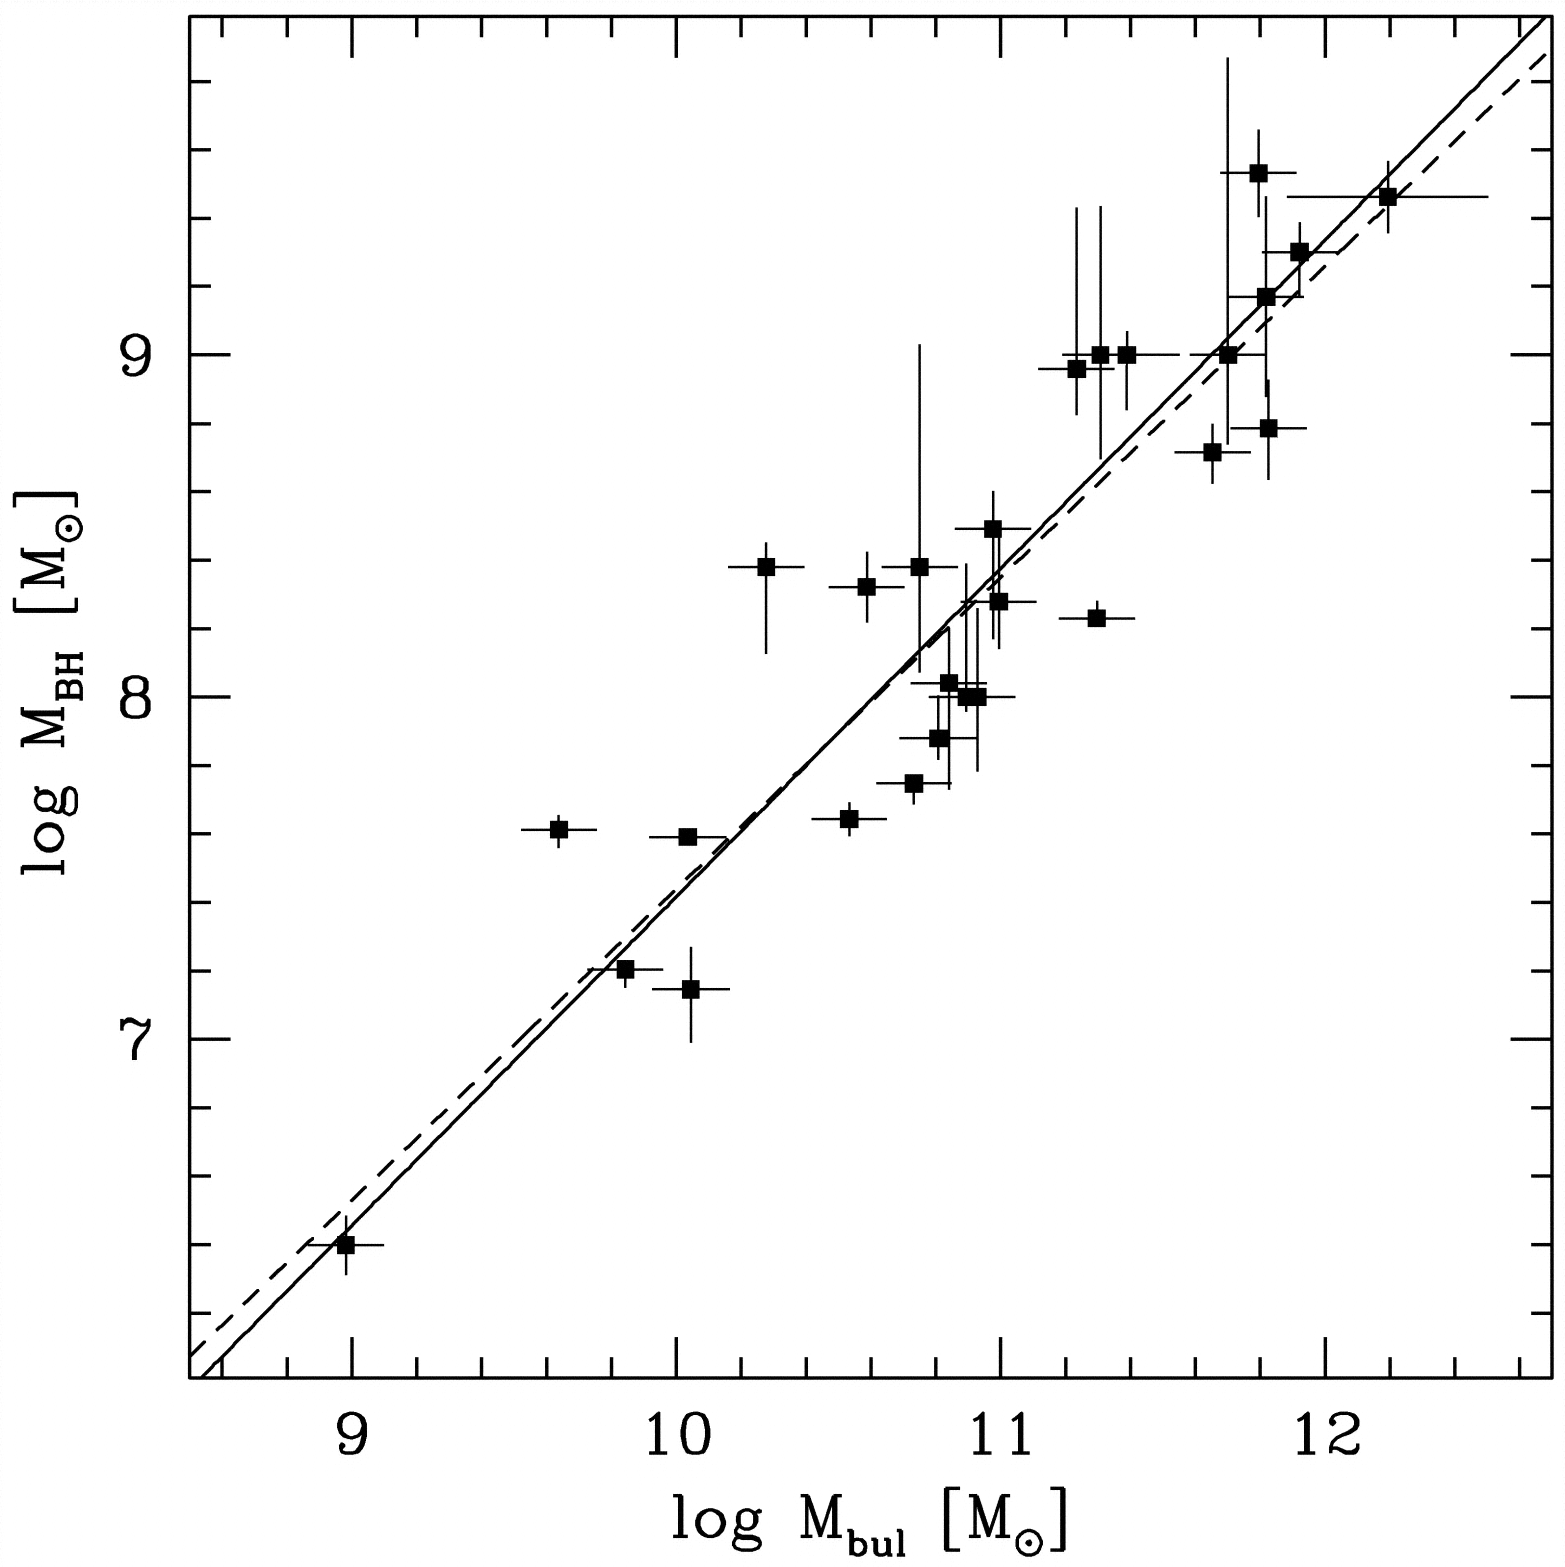
\includegraphics[width=\textwidth]{marconi_m-bul_2.png}
	\end{subfigure}
	\caption{Plots of both the $M_\bullet$ – $L_\mathrm{K,bulge}$ (left) and $M_\bullet$ – $M_\mathrm{bulge}$ (right) relations, alongside the observed data. The solid lines describe the relations given by equations \ref{eq:m-l_bulge} and \ref{eq:m-m_bulge}. The dashed lines are simple "least-squares" fits. The figures are adopted from \cite{Marconi2003}.}
	\label{figure:m-bulge}
\end{figure}

\section{Integral-Field Spectroscopy} \label{section:IFU}

Integral-field spectroscopy (IFS) has become an essential part of studying the kinematic properties of ETGs, as it allows for the spatial analysis of galactic spectra. IFS is conducted using instruments called "integral-field units", which in principle, calculate the spectrum of the observed light for each pixel. Often, however, the signal-to-noise ratio ($S/N$) of the singular pixels is quite poor. To improve the $S/N$, the pixel measurements are usually combined into so-called "spaxels" (i.e. spatial pixels) using an algorithm, such as the Voronoi-tessellation algorithm \citep{Cappellari2003}. This results in IFU-maps similar to figure \ref{figure:krajnovic_ifus}.

\begin{figure}
	\centering
	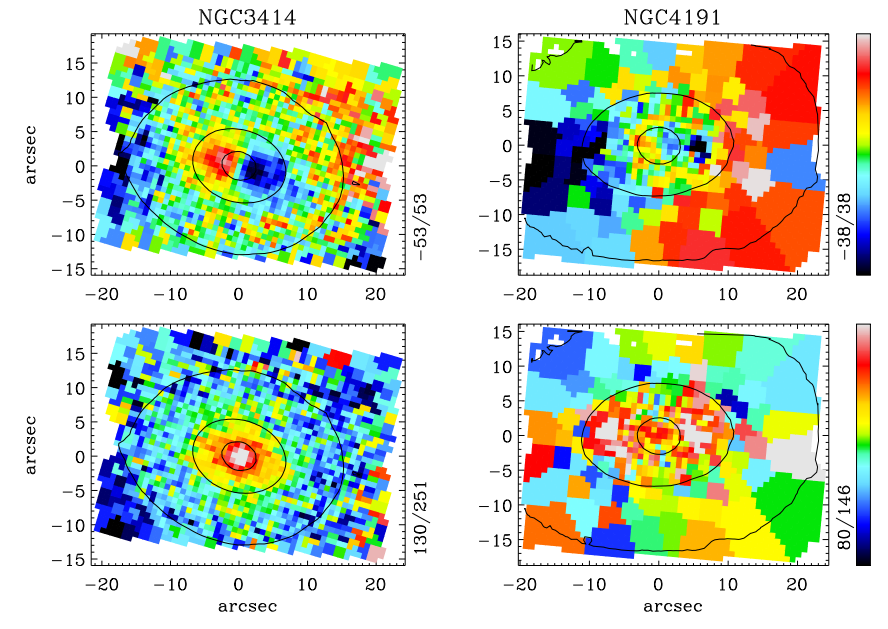
\includegraphics[width=0.9\textwidth]{krajnovic_ifus.png}
	\caption{IFU-maps of the mean line-of-sight velocities (top figures) and line-of-sight velocity dispersions (bottom figures) from the galaxies NGC 3414 and NGC 4191. The figures are adopted from \cite{Krajnovic2011}.}
	\label{figure:krajnovic_ifus}
\end{figure}

By creating a histogram out of the observed velocities in the pixels forming a spaxel, the spaxels can show the line-of-sight velocity distribution (LOSVD) of the regions in the observed galaxy that they encompass. The analysis of the LOSVDs is done by fitting the velocity histogram with some theoretical distribution function. Since the LOSVDs are usually similar to a Gaussian distribution function, but rarely purely Gaussian \citep{GalaxyFormationAndEvo2010}, the fitted distribution function is quite often (e.g. in the $\mathrm{SAURON}$ and $\mathrm{ATLAS^{3D}}$ projects, as well as the MASSIVE survey; \citealt{Bacon2001, Cappellari2011, Ma2014MASSIVE}) in the form of the modified Gaussian function \citep{VanDerMarel1993, Bender1994}:
\begin{equation}
f(v) = I_0 e^{-\gamma^2/2}(1 + h_3 H_3(y) + h_4 H_4(y)), \label{eq:mod_gaussian}
\end{equation} 
where $I_0$ is a normalization constant, $\gamma$ is the central slope of the particle density profile, $y = (v - V_\mathrm{avg})/\sigma$, and $H_3$ and $H_4$ are the third and fourth order Hermite polynomials respectively:
\begin{eqnarray}
H_3(y) = \left(2\sqrt{2}y^3 - 3\sqrt{2}y\right) / \sqrt{6}, \\
H_4(y) = \left(4y^4 - 12y^2 + 3 \right) / \sqrt{24}.
\end{eqnarray}
The four remaining parameters: the average LOS velocity $V_\mathrm{avg}$, the LOS velocity dispersion $\sigma$, and the third and fourth order Gauss-Hermite moments $h_3$ and $h_4$, which represent skewness and kurtosis respectively, are usually the parameters that are of interest.

By using IFS, a number of different kinematic features have been observed in ETGs. These features include: areas with low-level velocities or disk-like rotation, as well as regions where the kinematic axis of the galaxy is misaligned with its photometric axis \citep{Emsellem2007}. IFS has also helped identify so-called \textit{Kinematically Distinct Cores} (KDCs), which are central regions of galaxies with an angular momentum that has a different direction compared to the rest of the galaxy. There has also been evidence of \textit{Counter Rotating Cores} (CRCs), which are galactic cores that have a difference of around $180^\circ$ in the position angle of their angular momentum vector, when compared to their immediate surroundings \citep{Krajnovic2011}.

\subsection{Slow and Fast Rotators} \label{section:slow_fast_rotators}

Using LOSVD measurements done with IFS, \cite{Emsellem2007} have defined an explicit way to classify galaxies as either so-called slow or fast rotators. The basis for this classification is the $\lambda_R$ parameter, which describes the angular momentum of a galaxy, and is defined as:  
\begin{equation}
\lambda_R \equiv \frac{\langle R |V| \rangle}{\langle R \sqrt{V^2 + \sigma^2} \rangle}, \label{eq:general_lambdar}
\end{equation}
where $R$ is the projected distance from the galactic centre, $V$ is the line-of-sight velocity, $\sigma$ is the velocity dispersion and $\langle \; \rangle$ denote that the nominator and denominator in the equation are luminosity weighted means. From binned 2D kinematic maps, such as the ones given by IFS observations, this property can be calculated using the following formula:
\begin{equation}
\lambda_R = \frac{\sum^{N_p}_{i=1} F_i R_i |V_i|}{\sum^{N_p}_{i=1} F_i R_i \sqrt{V_i^2 + \sigma^2_i}}, \label{eq:binned_lambdar}
\end{equation}
where $F_i$, $R_i$, $V_i$ and $\sigma_i$ are the flux, projected distance from the galaxy centre, velocity and velocity dispersion of the $i$th bin, and $N_p$ is the number of bins.

Determining whether a galaxy is a fast or a slow rotator using $\lambda_R$, is done by comparing the value that the parameter gets at the galaxy's effective radius, to some pre-defined threshold. The originally used threshold is: $\lambda_{Re} < 0.1$, where $\lambda_{Re}$ is the $\lambda_R$-parameter at the effective radius, and where galaxies fulfilling this condition are classified as slow rotators \citep{Emsellem2007}. A revision of the threshold by \cite{Emsellem2011} takes the ellipticity ($\epsilon$) of the galaxy into account, and defines slow rotators as having $\lambda_{R_e} < 0.31 \sqrt{\epsilon}$, accounting for the increased anisotropy in the kinematics of flatter galaxies. An even further refinement of the slow rotator definition has been proposed by \cite{Cappellari2016}, where slow rotator galaxies are determined using the following two criteria: $\lambda_{R_e} < 0.08 + \epsilon/4$ and $\epsilon < 0.4$. The former criterion of the threshold reduces the risk of misidentifying very round non-regular slow rotators as fast rotators, while the latter makes sure that only sufficiently round galaxies are classified as slow rotators (Cappellari argues that "genuine" disk-less slow rotators are all rounder than $\epsilon = 0.4$).

Slow rotator galaxies, when defined using the above methods, often contain a KDC. In addition, they usually exhibit anisotropic velocity distributions, little to no large-scale rotation, kinematic misalignments and twists \citep{Emsellem2007, Cappellari2007}. The velocity distributions of fast rotators, on the other hand, are isotropic and their kinematic axis is aligned closely with their photometric axis \citep{Emsellem2007}. They also have disk-like kinematics and nearly oblate shapes \citep{Cappellari2007}. 

As expected, the dichotomy between slow and fast rotators clearly mirrors the kinematic differences between "boxy" and "disky" ellipticals. This implies that the cored and cuspy galaxies should follow the slow and fast rotator divide as well. \cite{Krajnovic2013} find that this indeed does seem to be the case, although there are a few exceptions. Nevertheless, even when accounting for these exceptions, \cite{Cappellari2016} considers the agreement to be good enough, for one to adequately draw conclusions about the photometry or kinematics of these galaxies, solely by whether they are classified as slow or fast rotators.

\section{Galactic Dynamics}

\subsection{Collisional And Collisionless Systems} \label{section:collisionless}

The motion of stars in stellar systems is caused by gravitational forces. However, due to the long-range nature of gravity, in expansive systems with a very large number of stars, the stellar motion is dominated by the gravitational influence of the numerous far-away stars, instead of a few strong close encounters. For this reason, when modelling such systems, it is often appropriate to ignore changes in the orbits of stars caused by specific stellar encounters, and simply approximate their motion as being caused by a smooth continuous gravitational potential. Systems where this approximation is applicable are called "collisionless systems", whereas systems where the modelling of the stellar motion requires knowledge about the gravitational effects caused by distinct massive particles, are called "collisional systems".

A stellar system can be approximated as collisionless if its "relaxation time" is significantly longer than its age. The relaxation time is defined, as the time it takes for the cumulative effect of encounters between a subject star and multiple field stars, to change the orbit of the subject star in such a significant way, that its initial conditions can not be inferred from its current motion. This process is often called "two-body relaxation". The relaxation time of a system can be calculated using the following formula \citep{BinneyTremaine}:
\begin{equation}
t_\mathrm{relax} \simeq \frac{0.1N}{\ln N} t_\mathrm{cross},
\end{equation}
where $N$ is the number of particles in the system, and $t_\mathrm{cross}$ is the crossing time, defined as the time it takes for a typical field-star to cross the system once.  The value of the crossing time can be estimated using the radius of the system $R$, and the typical field-star velocity $v$, as $t_\mathrm{cross} = R/v$. The relaxation times of galaxies are generally much longer than the age of the Universe ($\sim 13.8 \; \mathrm{Gyr}$). For example, the relaxation time of the solar neighbourhood is $t_\mathrm{relax} \simeq 6 \times 10^{14} \; \mathrm{yr}$. Thus, approximating galaxies as collisionless systems is a valid assumption.

Of specific interest to collisionless systems is the concept of "phase space". Phase space is a six-dimensional space, where in addition to the three basic Cartesian position coordinates ($x, y, z$), the possible states of a system are described by the three velocity coordinates ($v_x, v_y, v_z$). If all stars in a system have identical masses, these six dimensions can describe every dynamical state that a star can have. The state of the whole stellar system at a certain time $t$, can then be described using the stellar distribution function $f(\mathbf{x}, \mathbf{v}, t)$, also known as the phase space density. Thus, the use of phase space allows one to model the general motion in stellar systems, while neglecting to calculate the motion of specific stars.

In collisionless systems, stellar trajectories are smooth and continuous, making the motion of stars analogous to flowing fluid. Much like how the mass density of a fluid is conserved along the flow, the phase space density $f(\mathbf{x}, \mathbf{v}, t)$ is conserved around a star moving in the phase space. This means that the time-dependent behaviour of the system can be modelled using the "collisionless Boltzmann equation" \citep{MerrittBook}:
\begin{equation}
\frac{\partial f}{\partial t} + \mathbf{v} \cdot \nabla f - \nabla \phi \cdot \frac{\partial f}{\partial \mathbf{v}} = 0, \label{eq:CBE}
\end{equation}
where $\phi$ is the gravitational potential of the system. By integrating this equation over velocity, it is possible to derive equations which relate the gravitational potential of the stellar system to its moments of velocity distribution. These moments are statistical properties that can often be measured from observations. Thus, by using equation \ref{eq:CBE}, one can model the gravitational potential of a galaxy, without the knowledge of specific stellar orbits, through observations of the general stellar dynamics of a galaxy.
  
\subsection{Potential-Density Models} \label{section:potential_density}

When using the "collisionless system"-approximation to model a stellar system, knowledge about its gravitational potential is fundamental. If the mass-density distribution of the galaxy is known, the corresponding potential can be calculated from the Poisson's equation \citep{BinneyTremaine}:
\begin{equation}
\nabla^2 \phi = 4 \pi G \rho, \label{eq:poisson}
\end{equation}
where $\phi$ is the gravitational potential, $G$ is the gravitational constant, and $\rho$ is the aforementioned mass-density distribution. Different types of galaxies can, of course, have different mass distributions, which leads us to the so-called "potential-density models". These models describe galaxies using different density distributions, and then calculate their corresponding gravitational potential using the Poisson's equation. The initial mass-density distribution in the models is often derived in such a way, that it is able to account for properties observed in actual galaxies (e.g. the Dehnen model described below). 


One of the most popular potential-density models used when approximating elliptical galaxies, is the spherically symmetric Dehnen-model \citep{Dehnen1993}. The Dehnen-model is defined as:
\begin{equation}
\rho(r) = \frac{(3-\gamma)M}{4\pi} \frac{a}{r^\gamma (r+a)^{4-\gamma}}, \label{eq:dehnen_density}
\end{equation}
\begin{equation}
\phi(r) = \frac{GM}{a} \times 
\begin{cases}
	-\frac{1}{2-\gamma} \left[ 1 - \left( \frac{r}{r+a} \right)^{2-\gamma} \right] & \; \gamma \neq 2 \\
	\ln \frac{r}{r+a}	 & \; \gamma = 2
\end{cases},
\label{eq:dehnen_potential}
\end{equation}
where $M$ is the total mass, $a$ is the scaling radius, and $\gamma$ is the central slope of the profile. There are a few reasons why this model in particular is often used. Firstly, the density profile is a combination of two power-laws. This is similar to many observed luminosity and surface brightness profiles in Es (see section \ref{section:ellip_photo}), and also many simulated dark-matter profiles \citep{BinneyTremaine}. Furthermore, when projected, the outer parts of the density profile resembles the empirical "de Vaucouleurs" surface brightness profile. The model is also a generalization of two other commonly used potential-density models, namely the Jaffe-model and the Hernquist-model (these models can be derived from the Dehnen model by using $\gamma = 2$ and $\gamma = 1$, respectively; \citealt{Jaffe1983, Hernquist1990}). 

\section{Regularisation} \label{section:regularisation}

Simulations of, for example, the formation of low-luminosity cores by a SMBH binary merger, must take into account strong interactions between stars and black holes. Thus, these systems must be modelled as collisional. A common issue encountered in simulations of collisional systems, is the singularity at $r=0$ in the equation of motion \citep{BinneyTremaine}:
\begin{equation}
\ddot{r} = -GM/r^2, \label{eq:equation_of_motion}
\end{equation}
where $G$ is the gravitational constant, $M$ is the total mass of the two interacting particles, and $r$ is the distance between the particles. Often, when calculating the orbits of stars, simulations maintain accuracy by reducing the integration time-step when the accelerations of the simulated particles become large. In extremely close encounters, the singularity in equation \ref{eq:equation_of_motion} causes the accelerations to rise sharply, resulting in the use of smaller and smaller time steps, which effectively stops the simulation from progressing. 

The solution to this issue is regularisation. In a regularised system, the singularity in the equation of motion (equation \ref{eq:equation_of_motion}) is removed through a coordinate transformation. Two examples of such transformations are given by \cite{BinneyTremaine}, and detailed below.

The first example is the "Burdet-Heggie regularisation", which changes the simulation time $t$ to the fictitious time $\tau$, by using the relation: $\mathrm{d}t = r \; \mathrm{d}\tau$. It also adds the external gravitational field $g$ to the equation of motion. By applying these changes, it is possible to write the two-body equation of motion as:
\begin{equation}
\mathbf{r}'' - 2E_2\mathbf{r} = - \mathbf{e}+r^2\mathbf{g}, \label{eq:bh_eom}
\end{equation}
where $\mathbf{r}''$ is the second derivative of the position $\mathbf{r}$ with respect to the fictitious time $\tau$, $E_2$ is the energy of the two-body orbit, and $\mathbf{e}$ is the eccentricity vector. Equation \ref{eq:bh_eom} is similar to the equation of motion of an harmonic oscillator, and unlike equation \ref{eq:equation_of_motion}, it does not contain a singularity at $r=0$.

\begin{figure}
	\centering
	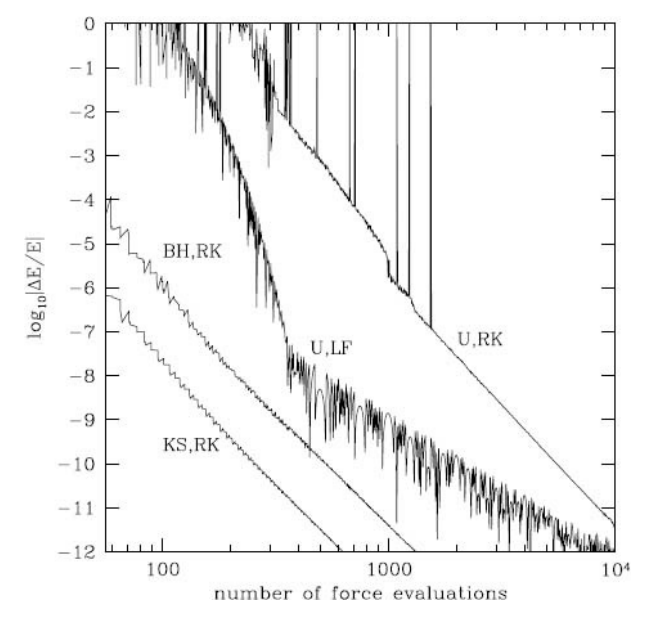
\includegraphics[width=0.7\textwidth]{binneytremaine_pic.png}
	\caption{Fractional error in the energy of a simulated orbit with an eccentricity of $e=0.99$, as a function of the number of force calculations per orbit. The errors were calculated after a single pericentre passage of the orbiting object. The multiple graphs denote the errors produced by different integrators and regularisation procedures. \textit{U}, \textit{BH} and \textit{KS} denote unregularised, "Burdet-Heggie" and "Kustaaheimo-Stiefel" regularisations, respectively. \textit{RK} and \textit{LF} then denote so-called "Runge-Kutta" and "Leapfrog" integrators, respectively. The figure is adopted from \cite{BinneyTremaine}.}
	\label{figure:regularized}
\end{figure}

The second example is the "Kustaaheimo-Stiefel" (KS) regularisation, which also converts the equation of motion of the two-body problem into an equation, similar to the equation of motion of a harmonic oscillator. However, in the case of the KS-regularisation, this is done by transforming the three-dimensional spatial coordinates into four-dimensional coordinates. 

Like the Burdet-Heggie regularisation, KS-regularisation defines a new fictitious time $\mathrm{d}t = r \; \mathrm{d}\tau$ and adds the gravitational field of the other particles to the equation of motion. The spatial coordinate transformation is done by changing the position vector $\mathbf{r} = (x, y, z)$ into a corresponding four-vector $\mathbf{u} = (u_1, u_2, u_3, u_4)$, where:
\begin{align}
\begin{split}
u_1^2& = \frac{1}{2}(x+r)\cos^2\psi \\
u_2^2& = \frac{yu_1+zu_4}{x+r} \\
u_3^2& = \frac{zu_1+yu_4}{x+r} \\
u_4^2& = \frac{1}{2}(x+r)\sin^2\psi,
\end{split}
\end{align}
and where $\psi$ is some arbitrary parameter \citep{BinneyTremaine}. When $\phi_e$ is the gravitational potential induced by the particles outside of the two-body problem, the equation of motion becomes as follows:
\begin{equation}
\mathbf{u}'' - \frac{1}{2} E \mathbf{u} = -\frac{1}{4} \frac{\partial}{\partial\mathbf{u}} \left( |\mathbf{u}|^2 \phi_e \right), \label{eq:ks_motion}
\end{equation} 
where $\mathbf{u}''$ denotes the second fictional time derivative of the four-vector, and $E$ is the energy of the two-body orbit when $\phi_e$ is taken into account:
\begin{equation}
E = \frac{1}{2}v^2 - \frac{GM}{r} + \phi_e = 2 \frac{|\mathbf{u'}|^2}{|\mathbf{u}|} - \frac{GM}{|\mathbf{u}|^2} + \phi_e.
\end{equation}
Equation \ref{eq:ks_motion} is now the equation of motion of a four-dimensional harmonic oscillator with an added external force \citep{BinneyTremaine}. Furthermore, as the equation in question clearly shows, the regularised form of the equation of motion is well defined even when the new position vector gets the value $\mathbf{u} = 0$. Thus, it does not contain the same singularity as the basic Cartesian version in equation \ref{eq:equation_of_motion}. Once this regularised version of the equation of motion has been used to calculate the motion of a particle, its new position in the four-dimensional space can be transferred back to three dimensions using the following relations:
\begin{align}
\begin{split}
x &= u_1^2 - u_2^2 - u_3^2 + u_4^2 \\
y &= 2 \left( u_1 u_2 - u_3 u_4 \right) \\
z &= 2 \left( u_1 u_3 + u_2 u_4 \right).
\end{split}
\end{align}

Figure \ref{figure:regularized} by \cite{BinneyTremaine}, compares the fractional errors in the energies of highly eccentric simulated orbits ($e = 0.99$) after one pericenter passage, integrated in differently regularised (or non-regularised) coordinates. The figure clearly shows how important the removal of the singularity is for the accuracy of the integration of the orbit. When using regularised coordinates, the integrators require around an order of magnitude less force evaluations to achieve the same accuracy, as when they are using unregularised coordinates. Furthermore, the efficiency of the integration is also clearly affected by the type of regularisation. Using the more robust KS-regularisation instead of the Burdet-Heggie regularisation scheme, results in a smaller fractional energy error.

\section{Post-Newtonian Dynamics} \label{section:PN}

When simulating mergers of galaxies that contain central SMBHs, general relativity has to be taken into account. Relativistic effects not only affect the orbits of stars that pass close to the black holes significantly, but are also required for the emission of the gravitational waves that drive the coalescence of the SMBH binary, during the final stage of its merger. However, the equations that describe these effects are difficult to solve, and thus inefficient to use in simulations. For example, effects on the motion of particles caused by the distortion of space-time near extremely massive objects, can not be modelled using a fixed linear background or common time-steps between all particles. Due to such complications, the effects caused by general relativity are often approximated using so-called "Post-Newtonian" (PN) dynamics.

PN dynamics is an extension of the basic Newtonian dynamics. It approximates the effects that Einstein's general theory of relativity has in the two-body problem, by adding so-called PN-terms to the Newtonian equation of motion. Each term has its own degree, describing increasingly precise relativistic effects. The magnitude of these effects are proportional to the order of $\mathbf{a}_\mathrm{xPN} \propto \left( v^2 / c^2 \right)^x$, where $x$ is the degree of the term in question. The resulting equation of motion is similar to:
\begin{equation}
\mathbf{a} = \mathbf{a}_\mathrm{Newtonian} + \mathbf{a}_\mathrm{1PN} + \mathbf{a}_\mathrm{2PN} + \mathbf{a}_\mathrm{2.5PN} + \ldots, \label{eq:PN_eom}
\end{equation}
where $\mathbf{a}_\mathrm{Newtonian}$ is the acceleration from the basic Newtonian equation motion, and $\mathbf{a}_\mathrm{xPN}$ are added PN corrections.

Depending on its degree, a PN-term either describes an effect that conserves the energy of the system, or an effect where energy is dissipated through gravitational radiation in the form of gravitational waves \citep{Mora2004}. Terms that have a degree that is an integer are conservative, while the half-degree terms are radiative and cause the orbit of a two-body system to shrink. For this reason, when simulating black hole mergers, it is imperative to include terms upto at least 2.5PN in the equation of motion.

The actual formulae for the PN-terms are quite long, and are thus not given here. They are derived from an expansion of Einstein's equations, based on the following two approximations. The interacting particles are assumed to be point masses, and the following equation is expected to hold true \citep{MerrittBook}:
\begin{equation}
\left( \frac{v}{c} \right)^2 \approx \frac{Gm}{c^2r} \ll 1, \label{eq:PN_assumption}
\end{equation}
where $G$ is the gravitational constant, $c$ is the speed of light, $m$ is the total mass of the two interacting particles, and $v$ and $r$ are the relative velocity and distance between the particles respectively. In words, equation \ref{eq:PN_assumption} represents two assumptions. Firstly, the velocities of the moving objects are assumed to be of the order that is expected for gravitaionally bound systems, and thus significantly slower than the speed of light. Additionally the objects are expected to never brought near the gravitational radius of one another \citep{MerrittBook}. 

An important caveat to note about the PN-approximation is that, the point mass assumption ignores the relativistic effects that the spin of the black hole, alongside its non-spherical shape, has on closely orbiting objects. Thus, in order to take them into account, one needs to add an additional spin PN-term to equation \ref{eq:PN_eom}. The effects caused by the spin of the black hole include orbital precession (i.e. changes in the rotational axis of the orbit), as well as precession of the spin itself \citep{Kidder1995}. The lack of spherical symmetry in the shape of the spinning BH, on the other hand, results in additional non-radial acceleration for the orbiting object \citep{MerrittBook}. However, the magnitude of this effect is very small.

\chapter{KETJU} \label{chapter:3}

KETJU \citep{Rantala2017KETJU} is a simulation code, designed for efficient and simultaneous modelling, of both galactic-scale dynamics and the precise motion of stellar particles near SMBHs. This is achieved through the combined functionality of two integrators with different degrees of efficiency and precision. The global dynamics of the simulated stellar system is calculated using the tree-integrator (section \ref{section:tree}) of the GADGET-3 simulation code \citep{Springel2005}, which in-turn uses softened dynamics (section \ref{section:softened_dynamics}) to calculate the general motion of particles in a collisionless system. The motion of bodies close to the SMBHs is, on the other hand, calculated using an algorithmically regularised chain method (AR-CHAIN, section \ref{section:ar-chain}; \citealt{Mikkola2008ARCHAIN}).

\section{Direct Summation and Tree Codes} \label{section:tree}

The simplest way of modelling the gravitational interactions between particles in a system, is to use the "direct summation" method. In the direct summation method, the gravitational force acted upon particle $\alpha$ is calculated using the basic Newton's law of gravity:
\begin{equation}
\mathbf{F}_\alpha = \displaystyle\sum_{\beta \neq \alpha} Gm_\beta \frac{\mathbf{r}_\beta-\mathbf{r}_\alpha}{|\mathbf{r}_\beta-\mathbf{r}_\alpha|^3}, \label{eq:f_alpha}
\end{equation}
where $m_\beta$ is the mass of the particle $\beta$, and $\mathbf{r}_\alpha$ and $\mathbf{r}_\beta$ are the vector positions of particles $\alpha$ and $\beta$, respectively. Since every particle contributes to the total gravitational force experienced by every other particle, when using this equation to calculate gravitational forces, the number of calculations needed to determine the motion of the entire system scales according to $N^2$, where $N$ is the total number of simulated particles. As a result, this method is very inefficient for simulations of systems such as galaxies, which may need millions of particles to adequately describe their internal dynamics. However, similar force-evaluation methods that only scale as $N\ln N$, also exist. One such method, included in GADGET-3 and used in the KETJU code, is the so-called "tree code".

\begin{figure}
	\centering	
	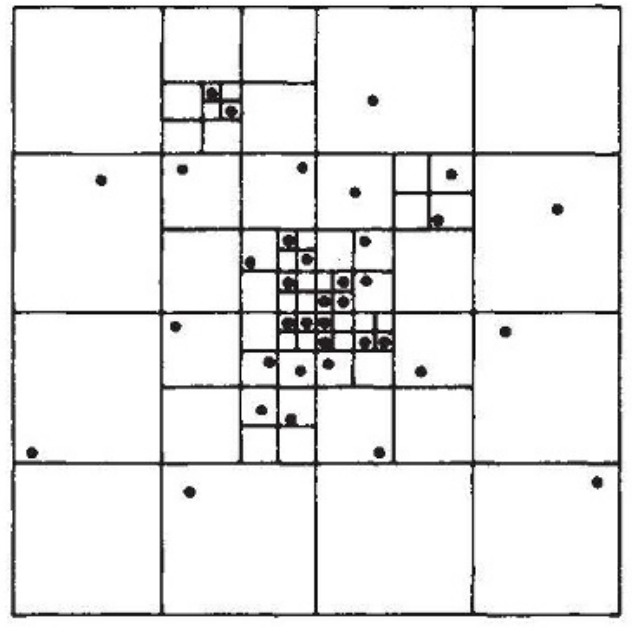
\includegraphics[width=0.6\textwidth]{barnes_octtree.png}	
	\caption{A 2D representation of the structure of an oct-tree. The squares represent the nodes, and the filled circles denote the location of the simulated particles. This figure is adopted from \cite{Barnes1986}.}
	\label{figure:oct_tree}
\end{figure}

In tree codes, the gravitational forces experienced by particles are not generated by the other particles themselves, but by so-called "nodes". These nodes are part of a structure called a "tree". In GADGET-3, this structure can be further specified as an "oct-tree", and is constructed as follows. First, the whole simulated system is enclosed in a single cubic volume called the "root" node. This cube is then divided into eight smaller cubic volumes called "child" nodes, and becomes their "parent" node. Next begins a recursive process, where child nodes that contain more than one particle, are divided into eight of their own respective child nodes. Nodes that contain a single particle are thus not divided into child nodes, and are called "leaf" nodes. The above process continues, until every single particle is located inside its own leaf node. The construction of any type of a tree structure follows the same basic principle outlined above. The variations in different tree types, come from the shape of the node-volumes and the number of volumes into which the nodes are subdivided. Figure \ref{figure:oct_tree} shows a two-dimensional representation of what an oct-tree would look like. 

The effect that a node has on the gravitational acceleration of a particle, is calculated with respect to its centre-of-mass. In GADGET-3, the gravitational force of the node is generated by the sum of the masses of the particles inside the node (i.e. the monopole moment of the node; \citealt{Springel2005}). However, it is also possible to calculate the force as the sum of the forces generated by the multipole moments of the node \citep{BinneyTremaine}:
\begin{equation}
\quad M_{ij} = \displaystyle\sum_\alpha m_\alpha x^\alpha_i x^\alpha_j; \quad M_{ijk} = \displaystyle\sum_\alpha m_\alpha x^\alpha_i x^\alpha_j x^\alpha_k,
\end{equation}
where $m_\alpha$ is the mass of the particle $\alpha$ inside the node; and $x_i^\alpha$, $x_j^\alpha$ and $x_k^\alpha$ are the components of the position vector of said particle, relative to the centre-of-mass of the node. Although only the quadrupole and octopole moments of the node are shown here, higher order multipole moments could also be used.

Of course, using the gravitational influence of every node to generate the acceleration of a particle would not make sense, as every parent node contains the same particles as its child nodes. Thus, which nodes are considered in the evaluation of the gravitational acceleration of a particle, are determined through a "tree walk". Starting from the root node and moving recursively through its child nodes, if a node fulfils an "opening criterion", it is taken into account in the force calculation. Otherwise the walk moves onto its child nodes. The original opening criterion described by \cite{Barnes1986} is the following:
\begin{equation}
\frac{l}{D} < \theta, \label{eq:opening_criterion}
\end{equation}
where $l$ is the length of the node, $D$ is the distance between the particle and the centre-of-mass of the node, and $\theta$ is some predetermined opening angle. Once all of the nodes that contribute to the acceleration of the particle have been determined, the gravitational influence that the system has on the motion of the particle, can be calculated as the sum of these force contributions. 

By using an opening criterion such as the one described in equation \ref{eq:opening_criterion}, individually weaker gravitational interactions from faraway particles are treated as though they were generated by a single bulk of mass. Thus, tree codes allow one to prioritise the calculation of significant gravitational effects induced by nearby particles, making the simulation of the whole system more efficient.

It is important to note that, in order to maintain accuracy, the tree structure must be reconstructed once the simulated particles have been propagated over a number of time-steps. How often this reconstruction is done, depends on the desired accuracy of the simulation. In simulation codes such as KETJU, which need to simulate dynamics with exceptionally high precision, the tree must be built after every integration step. Alongside the number of force calculations, the labour needed for the construction of the tree also scales according to $N \ln N$ \citep{BinneyTremaine}. However, even accounting for this additional work, when dealing with systems that contain a very large number of simulated particles, the use of the tree code is still far more efficient than the direct summation method, which has an $N^2$ scaling.

\section{Softened Dynamics} \label{section:softened_dynamics}

As equation \ref{eq:f_alpha} shows, the gravitational force between two massive point-masses starts to grow rapidly as the separation between them decreases. The removal of this divergence in the magnitude of the gravitational force is called "softening" the dynamics. The simplest example of softened dynamics is so-called Plummer softening, where the gravitational potential of a point-mass is described as:
\begin{equation}
\phi = -\frac{GM}{\sqrt{r^2 + \epsilon^2}}, \label{eq:plummer}
\end{equation}
and where $\epsilon$ is the "softening length". As one can see, using equation \ref{eq:plummer} to describe the gravitational potential causes the potential to converge at a constant value, as the separation $r \rightarrow 0$. However, the gravitational force generated by the Plummer potential is never exactly Newtonian. Thus, the use of this type of softening, inevitably introduces some errors into the motion of the simulated bodies.

When simulating the motion of multiple particles in a collisionless system, the use of softened dynamics is important. In simulations of galactic dynamics, the interacting particles are usually not representative of singular bodies. Often these particles are orders of magnitude more massive, and significantly less numerous, than for example the stars in a galaxy analogous to the simulated dynamical system. In such cases, the particles are generally used to depict phase space density. Their motion then describes the general motion of mass in the system, rather than the trajectories of specific stellar bodies. In fact, the initial positions and velocities of simulated particles are often generated through Monte-Carlo sampling (i.e. random sampling) of the phase space density distribution of the system. Due to their abnormally high mass however, strong interactions between two such particles, and the resulting changes in their motion, represent completely unphysical encounters. Thus, in order to make simulations of collisionless systems physically accurate, removing the divergence in the strength of the gravitational force is in fact necessary.

The tree code in GADGET-3 uses softened dynamics when calculating the gravitational forces between particles. In the code, the softening is done using a "Monaghan-Lattanzio" spline kernel \citep{Monaghan1985}, which gives an exactly Newtonian gravitational potential outside of the softening length $h_\mathrm{ML}$. The equation for the softened gravitational potential in the GADGET-3 tree code is \citep{Springel2001}:
\begin{equation}
\phi(r) = \frac{GM}{h_\mathrm{ML}} W \left(\frac{r}{h_\mathrm{ML}} \right), \label{eq:splinekernel_softened_potential}
\end{equation}
where $W$ is a spline-kernel defined as:
\begin{equation}
W(u) = 
\begin{cases}
\frac{16}{3}u^2 - \frac{48}{5} u^4 + \frac{32}{5} u^5 - \frac{14}{5} &\quad 0 \leq u < \frac{1}{2} \\
\frac{1}{15}u^{-1} + \frac{32}{3}u^2 - 16u^3 + \frac{48}{5} u^4 - \frac{32}{15} u^5 - \frac{16}{5} &\quad \frac{1}{2} \leq u < 1 \\
-\frac{1}{u} &\quad  1 \leq u
\end{cases}.
\end{equation} 
The length of $h_\mathrm{ML}$ is defined as $h_\mathrm{ML} = 2.8\epsilon$, where $\epsilon$ is the Plummer softening length. This makes the softened gravitational potential fully Newtonian beyond $r = 2.8 \epsilon$. In addition, the use of this softening length in particular, also makes the spline-kernel softened potential equivalent to the Plummer-potential at $r = 0$.

\begin{figure}
	\centering	
	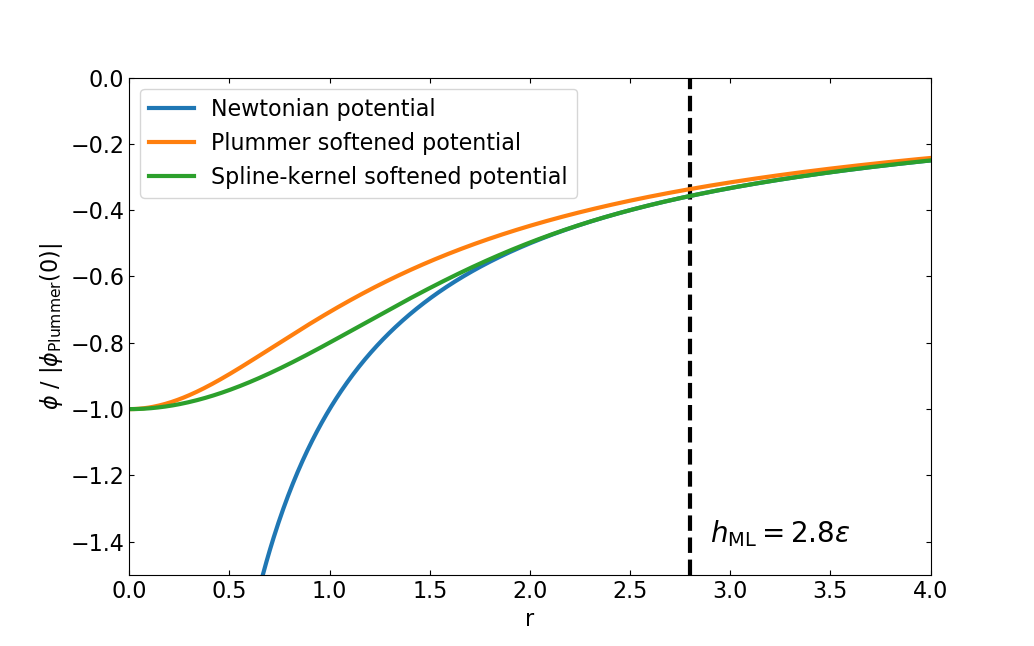
\includegraphics[width=0.9\textwidth]{softened_potentials.png}	
	\caption{Softened and pure Newtonian gravitational potentials as a function of distance. The potential on the y-axis is normalised so that, at $r=0$ the Plummer softened potential is $\phi_\mathrm{Plummer}(0) = -1$. The distance $r$ is given in units, where $G = M = \epsilon = 1$. The spline-kernel softening length is $h_\mathrm{ML} = 2.8 \epsilon$, and the vertical dashed black line shows the location at which $r = h_\mathrm{ML}$.}
	\label{figure:softened_potentials}
\end{figure}

Since the spline-kernel softened potential is equivalent to the purely Newtonian potential at distances beyond the softening length $h_\mathrm{ML}$, it provides a much more accurate estimation of galactic dynamics than the Plummer potential. Furthermore, the fact that the spline-kernel softening, similarly to Plummer softening, causes the potential to converge towards a constant value at $r=0$, it is also applicable in simulations of collisionless systems. Figure \ref{figure:softened_potentials} shows both of these properties. From the figure, one can also see that the spline-kernel softened potential seems to be all around more Newtonian than the Plummer potential, even at distances smaller than the softening length.


\section{AR-CHAIN} \label{section:ar-chain}

As stated above, KETJU uses an algorithmically regularised chain code (AR-CHAIN, \citealt{Mikkola2008ARCHAIN}) to simulate the dynamics near SMBHs with great accuracy. AR-CHAIN consists of three main components: regularisation of the few-body problem through time-transformed leapfrog integration, reduction of roundoff errors through the use of relative chain-coordinates, and the increase of its accuracy through Gragg-Bulirsch-Stoer extrapolation.

\subsection{Algorithmic Regularisation}

When simulating strong inter-particle interactions, a high numerical accuracy is often maintained through the use of adaptive time-steps. However, this raises the possibility that as the interactions become stronger, the time-steps become infinitesimally small and the simulation effectively stops progressing. Fortunately, this can be circumvented through the use of regularisation (see section \ref{section:regularisation}). 

In AR-CHAIN, the regularisation procedure employed is so-called "algorithmic regularisation". This scheme is based on different time-transformations for the equations of motion of the particle position, and every other time-dependent variable, respectively. The two fictitious times used in the regularisation are subtly different from each other, but should be identical along the exact solution of the $N$-body problem. For the particle positions, the time-transformation is given as \citep{Mikkola2008ARCHAIN}:
\begin{equation}
ds = [ \alpha ( T+B ) + \beta \omega + \gamma ] dt, \label{eq:ds_coords}
\end{equation}
while for the other, more velocity-like variables, the time-transformation is given as:
\begin{equation}
ds = [\alpha U + \beta \Omega + \gamma] dt. \label{eq:ds_vels}
\end{equation}
In the above equations, $s$ is the new fictitious time; $T$, $U$ and $B$, are the kinetic, potential and binding energies ($B = U - T$), respectively; $\alpha$, $\beta$ and $\gamma$ are variables, which determine the terms that are taken into account in the time-transformation (often, for example in KETJU, these parameters are set as $(\alpha, \beta, \gamma) = (1, 0, 0)$); $\Omega$ is an arbitrary function of the particle positions ($\Omega = \Omega(\mathbf{r})$); and the parameter $\omega$ is defined by the initial value $\omega(0) = \Omega(0)$, and the time dependence:
\begin{equation}
\dot{\omega} = \displaystyle\sum^N_i \frac{\partial \Omega}{\partial \mathbf{r}} \cdot \mathbf{v},
\end{equation}
where $N$ is the number of particles in the system. Since the time-transformations should be identical along the exact solution of the $N$-body equation of motion, it follows that, for the exact solution, the $\Omega$ and $\omega$ parameters should behave in the same way (i.e. $\Omega(t) = \omega(t)$). 

In the KETJU implementation of AR-CHAIN, the parameter $\beta$ is usually set as $\beta = 0$. This means that $\Omega$ and $\omega$ do not affect the time-transformation, and thus calculating their values is effectively optional. Still, following the time-evolution and convergence of these parameters is useful, as it allows one to examine how close to the exact solutions the equations of motion are being solved in the simulation, and update the simulation accuracy accordingly.   

The function usually used for $\Omega$ is similar to the potential energy, being defined as:
\begin{equation}
\Omega = \displaystyle\sum^N_i \displaystyle\sum^N_{j > i} \frac{\Omega_{ij}}{|\mathbf{r}_{ij}|}, \label{eq:ketju_omega}
\end{equation}
where $\mathbf{r}_{ij}$ is the distance between particles $i$ and $j$, and where the parameter $\Omega_{ij}$ is equivalent to the mass in the formula of the potential energy. The value of $\Omega_{ij}$ can determined using the equation:
\begin{equation}
\Omega_{ij} = 
\begin{cases}
\tilde{m}^2 &\quad m_i m_j < \epsilon_\Omega \tilde{m}^2 \\
0 &\quad \mathrm{otherwise}
\end{cases},
\end{equation}
where the quantity $\tilde{m}^2$ is the mean-mass product of the system:
\begin{equation}
\tilde{m}^2 = \frac{2}{N(N-1)} \displaystyle\sum^N_i \displaystyle\sum^N_{j > i} m_i m_j,
\end{equation}
and $\epsilon_\Omega$ is a user defined parameter. The value of this parameter is set to $\epsilon_\Omega = 10^{-3}$ in KETJU, meaning that only gravitational influences between particles with sufficiently small masses is taken into account when calculating $\Omega$. This is done in order to make sure that small bodies, which have a negligible impact on the total gravitational potential, can still have an effect on the regularisation. 

Using the two fictitious time definitions from equations \ref{eq:ds_coords} and \ref{eq:ds_vels}, allows us to form two sets of regularised equations of motion for the $N$-body problem. These equations consist of the coordinate equations:
\begin{equation}
\begin{split}
t' = \frac{dt}{ds} &= 1/(\alpha(T+B) + \beta\Omega + \gamma) \\
\frac{d\mathbf{r}_i}{ds} &= t' \mathbf{v}_i,
\end{split}
\end{equation}
and the velocity equations:
\begin{equation}
\begin{split}
\tilde{t}' = \frac{dt}{ds} &= 1/(\alpha U + \beta\omega + \gamma) \\
\frac{d\mathbf{v}_i}{ds} &= \tilde{t}' (\mathbf{a}_i + \mathbf{f}_i) \\
\frac{d\omega}{ds} &= \tilde{t}' \displaystyle\sum^N_i \frac{\partial \Omega}{\partial \mathbf{r}_i} \cdot \mathbf{v}_i \\
\frac{dB}{ds} &= -\tilde{t}' \displaystyle\sum^N_i \frac{\partial T}{\partial \mathbf{v}_i} \cdot \mathbf{f}_i, \\
\end{split}
\end{equation}
where $\mathbf{a}_i$ is the $N$-body acceleration, and $\mathbf{f}_i$ is the acceleration caused by perturbing gravitational forces, generated by bodies outside the $N$-body system that is simulated using AR-CHAIN. However, the gravitational force that produces the acceleration of the simulated particles is still Newtonian even in the time-transformed equations, and thus it is still not defined when $r=0$. Fortunately, this does not pose any practical problems for the simulations, as the calculations are done using floating point numbers. In this case, the probability for the value of the separation between two point masses being exactly $r=0$ is so small, that it is likely never to occur.

The final component of the algorithmic regularisation procedure is the leapfrog integrator. Generally, numerical orbit integration procedures consist of so-called "kick" and "drift" steps, where the dynamics of a simulated particle is updated according to the current state of the system, and where the particle is propagated according to its own current dynamical state, respectively. In the simplest possible integrator, when propagating a system over some time-step $\Delta t$, the particles are both kicked and then drifted once (or vice versa) over the whole time-step. In a leapfrog integrator, however, the preceding step is divided into two smaller steps over half of the total time-step, which are then calculated before and after the second step. We can help visualise this difference, by using $\mathbf{X}(\Delta t)$ and $\mathbf{V}(\Delta t)$ to notate the drift and kick steps, respectively. For the simple integrator, a single time-step would be:
\begin{equation}
\mathbf{X}(\Delta t)\mathbf{V}(\Delta t),
\end{equation} 
while a leapfrog time-step could be written as:
\begin{equation}
\mathbf{X}(\Delta t/2)\mathbf{V}(\Delta t)\mathbf{X}(\Delta t/2). \label{eq:DKD}
\end{equation}
Depending on which of the steps is divided into two, the integrator can either be a so-called "kick-drift-kick" (KDK) leapfrog, or a "drift-kick-drift" (DKD) leapfrog. The variant described by equation \ref{eq:DKD} is the DKD leapfrog, which is also the version used by KETJU \citep{Rantala2017KETJU}.

Using the time-transformation detailed above, a leapfrog integrator, and setting $(\alpha, \beta, \gamma)$ to $(1, 0, 0)$; AR-CHAIN is able to calculate exact two-body orbits, up to numerical accuracy \citep{Mikkola2008ARCHAIN}. However, simply using the algorithmic regularisation does not provide enough accuracy to calculate precise motion near SMBHs. Thus, it is imperative to improve the numerical accuracy of the integration through both, the usage of chain coordinates (section \ref{section:chained_coordiantes}), and an extrapolation method (section \ref{section:extrapolation}).

\subsection{Chained Coordinate System} \label{section:chained_coordiantes}

Apart from simple arithmetic operations with integers, all calculations done by computers contain roundoff errors, due to the finite accuracy of floating point numbers. When subtracting two numbers that have similar and very large values from each other, the effects caused by these errors can be significant. To reduce the size of the roundoff error, AR-CHAIN uses a chain coordinate system to calculate gravitational interactions between nearby particles. Instead of using, for example, centre-of-mass coordinates to calculate the gravitational forces, AR-CHAIN uses the relative positions between particles and their closest neighbour. This naturally decreases the size of the subtracted values, as the relative distance between two particles is likely significantly shorter, than their respective distances from the centre-of-mass of the system.

The chain coordinate system is constructed as follows. First, the particles that have the shortest distance from each other are identified. These particles are designated as the "tail" and the "head" of the chain. Next, the particle that is closest to either the head or the tail is added to the chain. This particle then becomes the new head or tail. This step is iterated over, until every particle in the system is included in the chain.

Once the chain has been formed, and the particles have been renamed from 1 to $N$ according to their position in the chain, $N - 1$ relative position and velocity vectors can be calculated using the following \citep{Mikkola2008ARCHAIN}:
\begin{equation}
\begin{split}
\mathbf{X}_k &= \mathbf{r}_{k+1} - \mathbf{r}_k \\
\mathbf{V}_k &= \mathbf{v}_{k+1} - \mathbf{v}_k.
\end{split}
\end{equation}
In the chained coordinate system, the basic equations of motion thus become:
\begin{equation}
\begin{split}
\dot{\mathbf{X}}_k &= \mathbf{V}_k \\
\dot{\mathbf{V}}_k &= \mathbf{A}_{k+1} - \mathbf{A}_{k} + \mathbf{f}_{k+1} - \mathbf{f}_{k},
\end{split}
\end{equation}
where $\mathbf{f}$ is the acceleration caused by external gravitational perturbations, and $\mathbf{A}$ is the total Newtonian gravitational acceleration induced by the other particles in the chain system, defined as:
\begin{equation}
\mathbf{A}_k = - \displaystyle\sum_{j \neq k} m_j \frac{\mathbf{r}_{jk}}{|\mathbf{r}_{jk}|^3}.
\end{equation}
The parameter $\mathbf{r}_{jk}$ in this equation, is the relative position from the subject particle $k$ to particle $j$. When using the chain coordinate system, this vector is as a sum of the chain distances from $j$ to $k$. However, naturally the sum of inter-particle vectors is seldom equivalent to the exact separation between two arbitrary particles in Cartesian coordinates. The errors caused by this can be significant for particles that are located far from each other in the chain. Thus, the use of chain coordinates improves the numerical accuracy of the acceleration, only when used for particles that are sufficiently close to each other. For faraway particles, the distance should still be determined using the basic Cartesian positions. Taking all this into account, the position vector $\mathbf{r}_{jk}$ is determined as follows \citep[e.g.][]{Rantala2017KETJU}:
\begin{equation}
\mathbf{r}_{jk} = 
	\begin{cases}
		\mathbf{r}_j - \mathbf{r}_k &\quad |j-k| > N_d \\
		\displaystyle\sum^{\mathrm{max} \{ j,k \}-1}_{i = \mathrm{min} \{ j,k \}} \mathrm{sign}(j-k) \mathbf{X}_i &\quad |j-k| \leq N_d
	\end{cases}, \label{eq:relative_dist}
\end{equation}
where $N_d$ denotes the maximum number of chain distances that can be used to determine the separation between two particles. \cite{Mikkola2008ARCHAIN} find that $N_d = 2$ produces the best results, and as such, the KETJU implementation of AR-CHAIN uses this same value.

In the chain coordinates, the time-transformed coordinate equations of motion can be written as:
\begin{equation}
\begin{split}
t'= \frac{dt}{ds} &= 1/(\alpha(T+B) + \beta\Omega + \gamma) \\
\frac{d\mathbf{X}_i}{ds} &= t' \mathbf{V}_i,
\end{split}
\end{equation}
while the velocity equations are:
\begin{equation}
\begin{split}
\tilde{t}' = \frac{dt}{ds} &= 1/(\alpha U + \beta\omega + \gamma) \\
\frac{d\mathbf{V}_i}{ds} &= \tilde{t}' (\mathbf{A}_i + \mathbf{f}_i) \\
\frac{d\omega}{ds} &= \tilde{t}' \displaystyle\sum^N_i \frac{\partial \Omega}{\partial \mathbf{X}_i} \cdot \mathbf{V}_i \\
\frac{dB}{ds} &= -\tilde{t}' \displaystyle\sum^N_i \frac{\partial T}{\partial \mathbf{v}_i} \cdot \mathbf{f}_i. \\
\end{split} \label{eq:chain_vel_coords}
\end{equation}
Using the chained variables in the equations of motion is not always convenient \citep{Mikkola2008ARCHAIN}. Thus, for example, the time-derivative of the binding energy (see final equation of the set in equation \ref{eq:chain_vel_coords}) is still evaluated using Cartesian velocities.

\subsection{Velocity Dependent PN-Corrections}

Since KETJU can be used to simulate dynamics near supermassive black holes, it takes relativistic effects into account. This is done in the form of additional post-Newtonian corrections to the equation-of-motion, up to order 3.5PN  \citep{Rantala2017KETJU}. As relativistic effects are dependent on the relative momentum between objects, the velocity of the simulated particle has to be considered when applying the PN-corrections. This results in the following equation of motion for the velocity of a particle:
\begin{equation}
\frac{d\mathbf{V}_i}{ds} = \tilde{t}' (\mathbf{A}_i + \mathbf{f}_i + g_i(\mathbf{v}_i)), \label{eq:velocity_eom_pn}
\end{equation}
where $g(\mathbf{v}_i)$ describe the additional acceleration experienced by the particle due to velocity dependent PN effects. In the case of an SMBH, it might also be useful to take into account how general relativity affects the spin of the particle. The equation of motion of the spin is: 
\begin{equation}
\frac{d\mathbf{S}_i}{ds} = \tilde{t}' \mathbf{S}_{\mathrm{PN},i} \times \mathbf{S}_i, \label{eq:spin_eom_pn}
\end{equation}
where $\mathbf{S}_i$ and $\mathbf{S}_{\mathrm{PN},i}$ are the spin of the particle and the spin PN-correction, respectively.

The fact that the addition of the velocity dependent acceleration causes the time-derivative of the velocity to be dependent on itself, means that it can not be integrated using conventional methods. In KETJU, this integration problem is solved through expanding the position-velocity phase space to include an "auxiliary velocity" $\mathbf{w}_i$, and using its chained counterpart $\mathbf{W}_i$ when necessary \citep{Rantala2017KETJU}. This allows one to separate the calculation of the time-derivative of the velocity from the velocity itself, by instead, using the auxiliary velocity when applying the accelerative PN-corrections \citep{Hellstrom2010, Pihajoki2015}.

The addition of $w_i$ to the phase space modifies the leapfrog integration-step slightly. At the beginning of the kick-step, both auxiliary velocities are set equal to their "physical" counterparts. Next, the physical velocities are kicked over half a time-step, while using the auxiliary velocities in the velocity dependent acceleration term. The new physical velocities are then used to update the auxiliary parameters over the whole time-step. Finally, the physical velocities are integrated over the remaining half-time-step, by applying the previously calculated auxiliary velocities for the velocity dependent terms. This gives an accurate value for the velocity, after the time-step $\Delta t$.

Using a notation similar to the one used for the basic leapfrog algorithm for the above velocity integration steps, the velocity dependent kick step can be written as:
\begin{equation}
\mathbf{V}(\Delta t/2) \mathbf{W}(\Delta t) \mathbf{V}(\Delta t/2).
\end{equation}
Thus, a single DKD leapfrog time-step, where velocity dependent forces are calculated with the help of auxiliary velocities is:
\begin{equation}
\mathbf{X}(\Delta t/2) \mathbf{V}(\Delta t/2) \mathbf{W}(\Delta t) \mathbf{V}(\Delta t/2) \mathbf{X}(\Delta t/2).
\end{equation}

Of course, while the use of auxiliary variables has only been discussed in terms of integrating the time-derivative of the velocity in this section, the procedure can also be used to solve other equations of motion. For example, the same self-dependence problem caused by the addition of PN-terms extends to the time-derivative of the spin of the black hole, as seen in equation \ref{eq:spin_eom_pn}. This issue can then be resolved, by expanding the phase space to include the auxiliary spin ($\mathbf{Z}$).

\subsection{Gragg-Bulirsch-Stoer Extrapolation} \label{section:extrapolation}

The final component in the high precision AR-CHAIN algorithm is the "Gragg-Bulirsch-Stoer" (GBS; \citealt{Gragg1965, Bulirsch1966}) extrapolation method, the use of which is crucial for the high numerical accuracy of the algorithm. The basic principle behind GBS-extrapolation is that; when integrating a function over a single time-interval, the integral is calculated multiple times, each time dividing the previously used time-step into two times as many smaller steps. When increasing the number ($n$) of these substeps, the integration accuracy increases, and the results should start to converge toward the exact solution. This exact solution can be estimated, by extrapolating the previously calculated results, and finding out what the solution would be at $n \rightarrow \infty$, i.e. when the length of time described by the subdivisions of the original integration time-step is infinitesimally small.

Implementing the GBS-extrapolation algorithm works as follows. Every time the function is integrated over the integration interval ($h$) using a different $n$, the results are extrapolated at $n \rightarrow \infty$ to get an approximation of the exact solution. In order to extrapolate the results, they are expressed as a function of the length of time described by the individual $n$ substeps used to calculate their value; that is, as a function of: $\Delta t = h/n$. Then, either a polynomial or a rational function is fitted onto these results. The value of the fit at $\Delta t = 0$, corresponds to the supposed exact solution of the integral at $n \rightarrow \infty$.

Whether the extrapolated result is good enough too be considered "exact", is determined by the user-specified error tolerance parameter $\eta_\mathrm{GBS}$, which should fulfil the condition:
\begin{equation}
\eta_\mathrm{GBS} \leq \bigg| \frac{T_{k+1} - T_k}{T_k} \bigg|, \label{eq:GBS_tolerance}
\end{equation}
where $T_k$ are previously extrapolated solutions to the integral, $k$ denoting the number of approximate integral solutions used in the extrapolation procedure when calculating the solution in question. The algorithm continues to iterate over $k$, calculating a new approximate solution of the integral using $n = 2^k$ substeps, and adding it to extrapolation procedure in order to get a more accurate value for the exact solution at $n \rightarrow \infty$, until equation \ref{eq:GBS_tolerance} holds true. Alternatively, if $k$ exceeds some predefined maximum value $k_\mathrm{max}$, the process starts from the beginning; the difference now being that, the initial integration interval is divided into two new initial intervals. The value that is able to fulfil the error tolerance condition, is then deemed the exact solution of the integral.

%In AR-CHAIN, the extrapolation algorithm works as specified above, and the integration over the individual $n$ substeps is naturally done using the chained leapfrog algorithm. The tolerance limit from equation \ref{eq:GBS_tolerance}, is taken into account when determining the extrapolated solution for any equation-of-motion.

\section{Basic Properties of KETJU}

In KETJU, the galactic dynamics is simulated as interactions between particles that represent either; the mass concentration of stars, dark matter or gas; or singular supermassive black holes. The combined functionality of the GADGET-3 tree code and the AR-CHAIN integrator, is then achieved by dividing these simulated particles into three different types: chain particles, perturber particles, and tree particles. The dynamics of the chain particles are simulated using the AR-CHAIN algorithm, and they correspond to the stars near an SMBH as well as the SMBH itself. The perturber and the tree particles, on the other hand, are propagated using the GADGET-3 tree code, and they describe the general dynamics of the simulated stellar system at larger scales. The difference between the perturbers and the tree particles is that, the former are located close enough to the SMBH particle to have a significant individual effect on the dynamics of the chain particles. The type of a particle is determined by its distance from an SMBH. However, as of the current version of the KETJU code, only stellar and SMBH particles can be categorised as chain particles. An illustration of the different particle type regions around an SMBH particle can be seen in figure \ref{figure:ketju_regions_illustration}.

\begin{figure}
	\centering	
	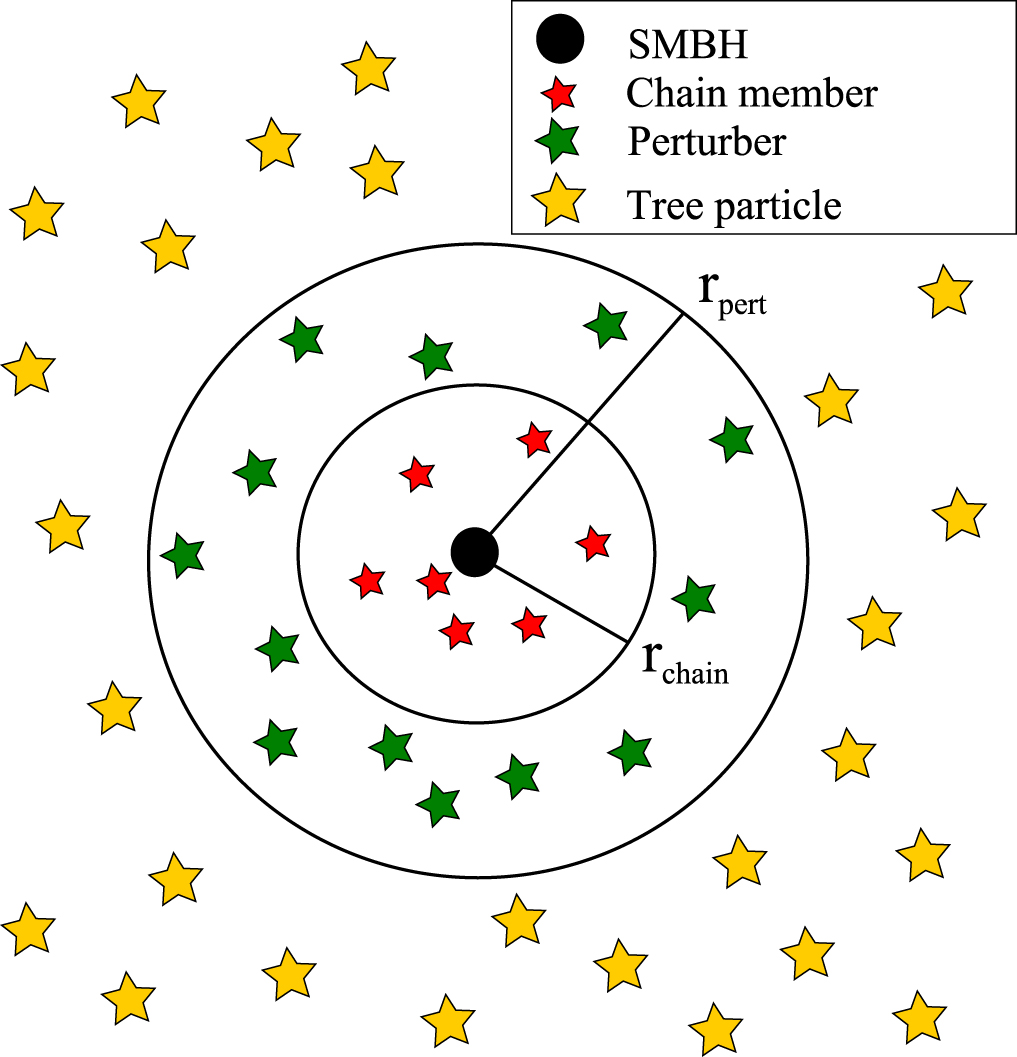
\includegraphics[width=0.6\textwidth]{rantala2017.jpg}	
	\caption{An illustration of the way KETJU divides the simulated particles into three different types. The red stars denote the chain particles, while the green and yellow stars show perturber and tree particles, respectively. The black dot is the SMBH particle, and the circles correspond to the regions, which determine the particle type. This figure is adopted from \cite{Rantala2017KETJU}.}
	\label{figure:ketju_regions_illustration}
\end{figure}

\subsection{The Chain Subsystem}

In simulations that deal with supermassive black holes, it is of utmost importance, that the dynamics of the SMBH particles are never softened. Softened gravitational potentials naturally induce weaker gravitational interactions, reducing the strength of effects such as dynamical friction, and thus unnaturally lengthening the time-scale of the SMBH binary inspiral and merger. In KETJU, the non-softened interactions between the SMBH particles are enforced through the combined use of a "chain subsystem", the internal dynamics of which are calculated using the AR-CHAIN, and "Monaghan-Lattanzio" (ML) spline-kernel softening (see section \ref{section:softened_dynamics}). 

A chain subsystem is made up of an SMBH particle and its surrounding chain particles. Whether a stellar particle is included in the subsystem as a chain particle, is determined through a variable called the "chain radius", defined as \citep{Rantala2017KETJU}:
\begin{equation}
\frac{r_\mathrm{chain}}{1 \; \mathrm{kpc}} = \lambda \times \frac{M_\bullet}{10^{10} M_\odot},
\end{equation}
where $M_\bullet$ is the mass of the SMBH particle, and $\lambda$ is a user-specified parameter. If the distance from a stellar particle to an SMBH particle is smaller than the chain radius, it is included in the chain subsystem of the black hole in question. Additionally, the condition $r_\mathrm{cahin} > h_\mathrm{ML}$ (where $h_\mathrm{ML} = 2.8\epsilon$ is the "Monaghan-Lattanzio" softening length employed in KETJU) is taken into account when determining the length of the chain radius. Since the dynamics of particles beyond the softening length is exactly Newtonian when using ML-softening, this ensures that gravitational interactions between SMBHs and stars, as well as other SMBHs, are never softened.

In the tree code, the chain subsystem behaves as a single collisionless "macro particle". The motion of this macro particle is calculated using the centre-of-mass properties of the subsystem. In order to get the centre-of-mass acceleration of the subsystem, the tree-accelerations of all of the particles included in the chain are calculated. This means that, somewhat counter-intuitively, even though the chain particles are propagated in the tree as a single macro particle, they are "seen" as separate by the other tree-particles.

Since every SMBH has its own regularised region, if two SMBH particles are close enough to each other, it is possible for two chain subsystems to merge. This occurs, when the volumes of the subsystems intersect. A merged chain subsystem behaves similarly to a basic regularised region, where all of the chain particles are included in a single chain in the AR-CHAIN algorithm. In the case of a merged subsystem, the inclusion of stellar particles as chain particles is determined by checking the condition for both SMBHs.

\subsection{Perturbative Effects of the Perturber and Tree Particles}

When calculating the precise motion of the chain particles in the regularised regions around SMBHs, it is important to take into account tidal perturbation caused by the gravitational influence of the other particles in the simulated stellar system. Both the aforementioned perturber and tree particles induce tidal perturbations, however, the way these effects are considered when propagating the chain particles, depends on the respective particle type. When calculating these effects, the gravitational forces induced by the softened gravitational potential (equation \ref{eq:splinekernel_softened_potential}) of the tree-code are used.

The perturber particles are located outside of the regularised region, but lie close enough to the chain particles to have a significant individual perturbative effect on their equations of motion. In KETJU, a tree-particle is deemed to be a perturber, if it is located inside the "perturber radius" \citep{Rantala2017KETJU}:
\begin{equation}
r_{\mathrm{pert},i} = \gamma \left( \frac{m_i}{M_\bullet} \right)^{1/3} r_\mathrm{chain},
\end{equation}
where $m_i$ is the mass of a potential perturber particle, and $\gamma$ is a user-specified parameter, that is set so, that $r_{\mathrm{pert},i} = 2r_\mathrm{chain}$ for the lowest-mass simulated particles. Naturally, chain subsystems can be perturbed by other chain subsystems. In case this happens, the perturbative subsystems are resolved, and the gravitational effects of individual chain particles are calculated.

Since the perturber particles are located close to the chain subsystem, the tidal perturbation induced by them depends significantly on their location in respect to the chain particles. This is problematic when calculating the trajectories of the chain particles using AR-CHAIN, as the integration time-steps used in the algorithm are smaller than the time-step used for the propagation of the perturber particles (see section \ref{section:archain_plus_gadget}), making the perturbers effectively stationary during the AR-CHAIN integration procedure. To remedy this, the time-evolution of the position of the perturber particles is estimated using following quadratic equation:
\begin{equation}
\mathbf{r}(t) = \mathbf{r}(t_0) + \mathbf{v}(t_0)\Delta t + \frac{1}{2}\mathbf{a}(t_0) (\Delta t)^2,
\end{equation}
where $t_0$ is the moment in simulation time, at which the AR-CHAIN integration procedure starts; $\mathbf{r}(t_0)$, $\mathbf{v}(t_0)$ and $\mathbf{a}(t_0)$ are the initial position, velocity and acceleration of a perturber particle, respectively; and $\Delta t$ is the time elapsed form $t_0$, i.e. $\Delta t = t - t_0$. The tree particles, on the other hand, are estimated to be stationary during the whole integration time-step. This approximation is valid, as the scale of the tree-particle region is so large, that small variations in the positions of the individual particles do not have a significant effect on the total perturbative force \citep{Ahmad1973}.

Naturally, as the perturber and tree particles exert a gravitational force onto the chain particles, they must experience an equal and opposing force from the particles in the subsystem (as stated by Newton's third law). This is taken into account in KETJU, by substituting the gravitational acceleration induced by the chain subsystem macro particle onto the perturbative particle, with the total gravitational force from the individual chain particles. This gravitational force is calculated with the direct summation method (see section \ref{section:tree}), using Monaghan-Lattanzio spline-kernel softening (equation \ref{eq:splinekernel_softened_potential}).

\subsection{Particle Mergers}

In KETJU simulations, it is possible for an SMBH particle to merge with a stellar particle or another SMBH particle. Whether the merger event occurs, is determined by two possible criteria. The first criterion compares the gravitational wave coalescence time-scale for an SMBH binary to the tree code time-step, and is thus only relevant for SMBH-SMBH mergers. The coalescence time-scale can be approximated using \citep{Rantala2017KETJU}:
\begin{equation}
t_c \sim -\frac{a}{4\dot{a}},
\end{equation}
where $a$ is the semi-major axis of the binary orbit, and $\dot{a}$ is its time derivative, which (as shown in section \ref{section:gravitational_radiation}) can be calculated using post-Newtonian corrections at order 2.5PN as:
\begin{equation}
\left\langle \frac{da}{dt} \right\rangle = -\frac{64}{5}\frac{G^3M_1M_2(M_1+M_2)}{c^5a^3(1-e^2)^{7/2}} \left( 1+\frac{73}{24}e^2+\frac{37}{96}e^4 \right).
\end{equation}
If the condition $t_c < s_1 \Delta t_\mathrm{tree}$, where $s_1 > 1$ is a temporal safety factor (usually $s_1 = 10$), holds true; the two SMBH particles are merged.

The second criterion is based on the relative position of the two particles. For two SMBHs, the merger event is set to occur, if their separation is smaller than: 
\begin{equation}
r_\mathrm{min,S} = 6\left( \frac{2GM_{\bullet,1}}{c^2} + \frac{2GM_{\bullet,1}}{c^2} \right), \label{eq:bh_binary_merger_cond}
\end{equation}
which corresponds to the sum of the Schwarzschild-radii (i.e. the distance from a black hole at which the escape velocity is equivalent to the speed of light) of the binary pair multiplied by six. The seemingly arbitrary multiplication of the condition, comes from the fact that the use of PN dynamics is based on the approximation that $v/c \ll 1$. At small binary separations, the orbital velocities of the SMBHs naturally rise, which might invalidate the use of the PN-approximation. Through testing, \cite{Rantala2017KETJU} find that PN-dynamics is still valid at distances corresponding to equation \ref{eq:bh_binary_merger_cond}. 

In the case of an SMBH - stellar particle merger however, depending on which of the parameters is larger; the minimum particle separation is determined either using the Schwarzschild radius of the SMBH, or the tidal disruption radius (i.e. the distance from the black hole, where its gravitational force tears an orbiting star apart). The minimum distance between an SMBH particle and a stellar particle is determined by the following equation:
\begin{equation}
r_\mathrm{min,T} = \mathrm{max} \left\lbrace \frac{12GM_{\bullet}}{c^2}, \; s_2 R_\odot \left( \frac{M_\bullet}{M_\odot} \right)^{1/3} \right\rbrace,
\end{equation}
where $M_\odot$ and $R_\odot$ are the solar mass and radius, respectively, and $s_2 > 1$ is the spatial safety factor. 

The particle mergers are checked before every integration time-step. If either of the SMBH-SMBH merging conditions are met, the simulated particles are replaced by a new particle with the following properties \citep{Rantala2017KETJU}:
\begin{equation}
\begin{split}
M &= M_1 + M_2 \\
\mathbf{r} &= (M_1 \mathbf{r}_1 + M_2 \mathbf{r}_2) / M \\
\mathbf{v} &= (M_1 \mathbf{v}_1 + M_2 \mathbf{v}_2) / M \\
\mathbf{L} &= \frac{M_1 M_2}{M} (\mathbf{r}_2 - \mathbf{r}_1) \times (\mathbf{v}_2 - \mathbf{v}_1) \\
\mathbf{S} &= \mathbf{L} + \mathbf{S}_1 + \mathbf{S}_2,
\end{split}
\end{equation}
where $\mathbf{L}$ is the angular momentum, and $\mathbf{S}$ is the spin of the SMBH (however, note that in KETJU simulations (e.g. the ones described in chapter \ref{chapter:4}), the spin is often not taken into account, as its effects on the stellar dynamics are not significant). However, if an SMBH particle and a stellar particle merge, the stellar particle is simply removed from the simulation.

\subsection{Incorporating AR-CHAIN in the GADGET-3 Leapfrog} \label{section:archain_plus_gadget}

The GADGET-3 tree-code integrator used in KETJU is a KDK-leapfrog \citep{Springel2005}. Implementing the regularised chain region in the leapfrog integration works as follows. The first step, before starting the integration cycle itself, is naturally to determine the particle types for all particles in the simulated system and find the chain subsystem macro particles. 

Next, the particles that have been designated as either tree, perturber or macro particles, are kicked and drifted as expected in a KDK-leapfrog. After the drift-step, the chain particles are propagated using the chain integrator. Once the AR-CHAIN algorithm has concluded its calculations, the final kick step of the GADGET-3 leapfrog takes place. Lastly, the force corrections on the peruturbing particles, necessitated by the Newton's third law, are taken into account. 

The GADGET-3 leapfrog in KETJU, uses individual adaptive time-steps for different particles, the lengths of which can be determined using:
\begin{equation}
\Delta t_\mathrm{grav} = \left(\frac{2\eta \epsilon}{|\mathbf{a}|} \right)^{1/2},
\end{equation}
where $\mathbf{a}$ is the acceleration of a particle, $\epsilon$ is the gravitational softening length, and $\eta$ is a user-specified error tolerance parameter. These time-steps are then rounded down to the nearest discrete power-of-two time-step:
\begin{equation}
\Delta t_n = 2^n \Delta t_\mathrm{min},
\end{equation}
where $\Delta t_\mathrm{min}$ is the smallest possible time-step allowed by the simulation. 

The time-steps of the individual tree-particles are determined using the above procedure. The chain subsystem macro particles and the individual chain particles that are integrated using the AR-CHAIN algorithm, are placed onto the smallest tree time-step. This time-step is used as the initial integration interval in the AR-CHAIN integration. Using the smallest time-step from the tree code for the chain particles, ensures that they are active at all times during the simulation, and that they are on the smallest time-step if they happen to leave the chain region. The perturber particles are also placed on the smallest tree particle time-step. This is done in order to make sure that they are synchronised with the chain particles. 

%\section{Merging of Black Hole Particles}

%Since we are trying to determine if merging SMBH binaries form cores in merger remnants, we must make sure that the progenitors' central black holes actually merge in our simulations. This is done by looking at the "Run" simulations, as they contain the locations of the black holes from multiple time steps, and as the "Snapshots" still show both of the SMBHs.

%Plotting the positions of the black holes from "Run 3" in coordinates centred on the binary's centre-of-mass during the initial time step gives us figure \ref{figure:run3_traj}. Even by eye, one can clearly see that the orbit of the black hole with a smaller mass becomes smaller and smaller as the binary moves further away from its initial position. While this doesn't explicitly tell us that the black holes merge into each other, it does indicate the existence of a hardening process in the binary. Similar figures to figure \ref{figure:run3_traj} from all four "Runs" can be found in the appendix (figure \ref{figure:all_traj}).

%\begin{figure}[h]
%	\centering	
%	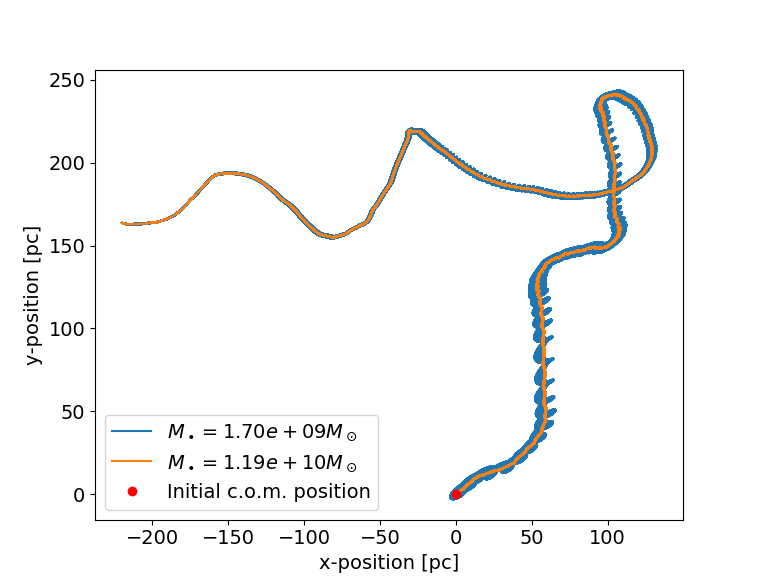
\includegraphics[width=0.7\textwidth]{Run3_Trajectory.png}	
%	\caption{The trajectories of the black holes during "Run 3". The coordinates are centred on the initial location of the centre-of-mass of the binary black hole. The orange and blue lines show the paths taken by the smaller and larger black holes respectively. Both paths show clear spiral patterns which become smaller and smaller as the simulation proceeds. The paths end at the location where the black holes merge, i.e. where the distance between them is $\lesssim 100 R_s$ ($R_s$ is the Schwarzschild radius).}
%	\label{figure:run3_traj}
%\end{figure}

%\begin{figure}[h]
%	\centering
%	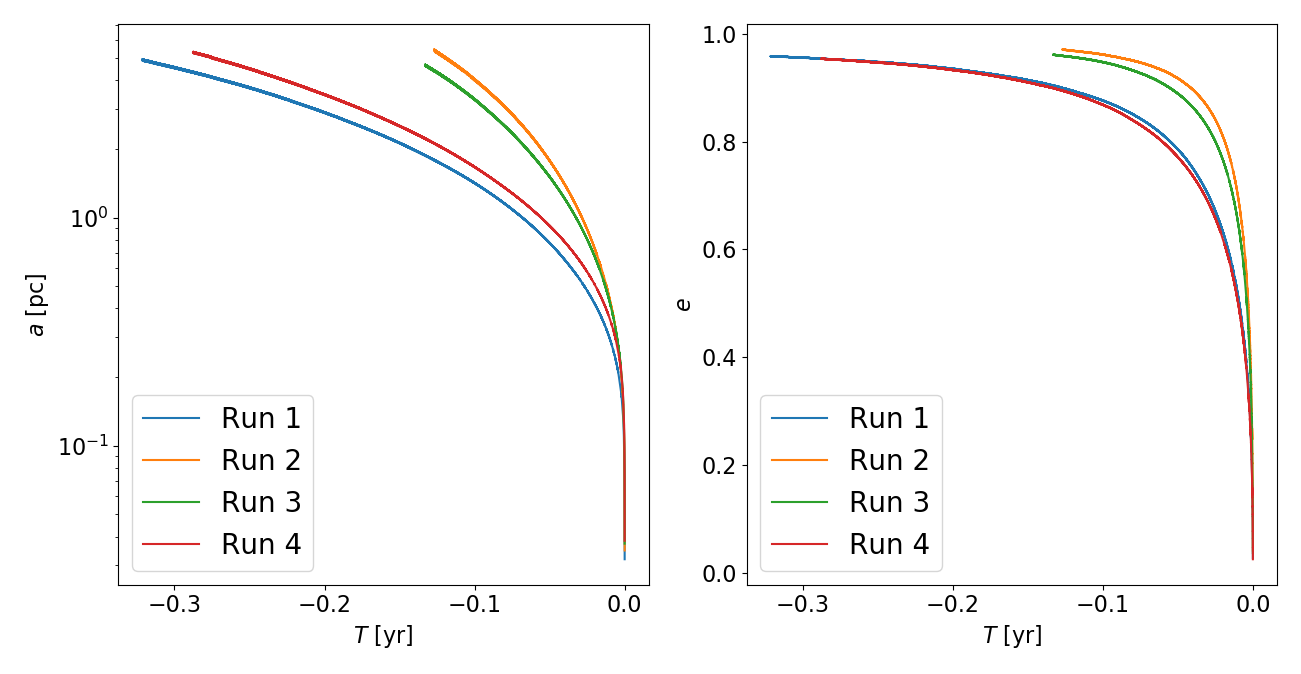
\includegraphics[width=\textwidth]{semi_major_and_ecc.png}
%	\caption{The semi-major axes (left) and eccentricities (right) of the black hole systems in the simulations "Runs 1"-"Run-4" as a function of time. The zero position on the x-axis corresponds to the point in simulation time, where the black hole merging event occurs.}
%	\label{figure:semi_and_ecc}
%\end{figure}

%The most likely obstacle for the complete merging of the binary black holes is the so-called final-parsec problem; where, due to the lack of stellar material that can be ejected during the three-body scattering phase, the hardening of the binary stops when the separation between the two black holes is $\sim 1 \mathrm{pc}$. This is assumed to happen since, not only is the binary constantly ejecting the finite amount of stars inside the loss-cone (defined in section 2), but the loss cone itself is becoming smaller due to the contracting binary orbit.

%Figure \ref{figure:semi_and_ecc} shows the time evolution of both the semi-major axis and the eccentricity of the binary orbits from all of the simulation runs. Interestingly enough the semi-major axes of all of the binaries go far below single parsec scales, meaning that the final-parsec problem doesn't seem to play a part in the simulations. This implies that, there exists some loss-cone refill mechanism which allows the binary to eject more stellar material than what initially exists inside the loss cone.



\chapter{Simulating Core Formation Using KETJU} \label{chapter:4}

This chapter consists of the description and my analysis of seven galaxy merger simulations run by \cite{Rantala2018} using the KETJU code. In all but one simulation, the merger progenitor galaxies contain central supermassive black holes, which form a hard binary during the merger event. These binaries are a likely source for the observed low-luminosity cores, as they can eject stars from the galactic centre through complex three-body interactions. The goal in this chapter is to determine if there is a connection between the central binary SMBH and the existence of a low-luminosity core, and if the simulated KETJU results agree with observations of cored galaxies.

\section{Simulation Details}

The simulation sample run by \cite{Rantala2018} includes seven different equal-mass mergers of two identical galaxies. The merger progenitor galaxies used in the different simulations (named BH-0 - BH-6), consist of equal mass stellar particles and equal mass dark matter particles, where the mass of the stellar particles differs from the mass of the dark matter particles. The progenitors are gas free (i.e. the simulations describe so-called "dry" mergers), and all of them but one contains an SMBH at their centre.

The initial conditions (ICs) of the merger progenitor galaxies are modelled as multicomponent, spherically symmetrical stellar systems. They consist of the three aforementioned components: stellar particles, dark matter particles and a central SMBH. The central SMBH is modelled as a single point mass located at the origin of the internal coordinate system of the host galaxy. On the other hand, the stellar and dark matter components consist of multiple particles, and are distributed according to their own spherically symmetric Dehnen density-potential models (\citealt{Dehnen1993}; see equations \ref{eq:dehnen_density} and \ref{eq:dehnen_potential} in section \ref{section:potential_density}). An important difference in the models used for the stellar and dark matter particles, is the value of the central slope ($\gamma$) of the mass-density profile. For stellar particles the $\gamma$-parameter is set to $\gamma = 3/2$, while for the dark matter particles the value of $\gamma = 1$ is used.

When constructing the multicomponent ICs for the progenitor galaxies (this procedure will be discussed in detail later in this section), the positions of the stellar and dark matter particles are determined using their respective cumulative mass profiles. These mass profiles are derived using the aforementioned Dehnen density-potential model, and can be written as:
\begin{equation}
M(r) = 4\pi \int^r_0 \rho(r)r^2 \;dr = M \left( \frac{r}{r+a} \right)^{3-\gamma}, \label{eq:cumulative_mass}
\end{equation}
where $\rho(r)$ is the density profile of the model (equation \ref{eq:dehnen_density}), and $a$ is the scaling radius.

In equation \ref{eq:cumulative_mass}, the value of the scaling radius ($a$) is determined quite differently for stellar and dark matter particle distributions. One way of calculating $a$ is to derive the formula of the half-mass radius from the cumulative mass profile. This results in the equation:
\begin{equation}
r_{1/2} = a \left( 2^{1/(3-\gamma)}-1 \right)^{-1}, \label{eq:half-mass-radius}
\end{equation}
from which $a$ can be solved easily. However, in order to get a value for $a$, one now needs to know the half-mass radius of the particle distribution. Fortunately, the half-mass radius of the stellar population can be determined through drawing an equivalence between it and the effective radius of the galaxy. If the galaxy, for which one is trying to determine the scaling radius, has a constant mass-to-light ratio, its mass and light profiles are proportional to each other. In this case, the properties described by the two profiles are analogous, which means that the half-mass radius and the effective radius are equivalent to each other. In cases, such as our simulations, where only the 2D projection of the effective radius is known, the three dimensional half-mass radius can be approximated using the following formula:
\begin{equation}
R_e \approx \frac{3}{4} r_{1/2}, \label{eq:projection_approximation}
\end{equation} 
where $R_e$ is the aforementioned 2D projected effective radius. Thus, knowing the effective radius of the galaxy allows one to determine the stellar scaling radius $a_\star$, by using both equation \ref{eq:half-mass-radius} and \ref{eq:projection_approximation}.

The scaling radius of the dark matter particle distribution can be derived using the dark matter fraction ($f_{\mathrm{DM}}$) inside the stellar half-mass radius. The dark matter fraction describes the fraction of the total mass inside radius $r$ that is contributed by dark matter, and is defined by the following equation:
\begin{equation}
f_\mathrm{DM}(r) = \frac{M_\mathrm{DM}(r)}{M_\star(r) + M_\mathrm{DM}(r)}. \label{eq:dm_fraction}
\end{equation}
With the above equation, one can get the dark matter scaling radius by substituting the cumulative mass profiles in the equation with the one from equation \ref{eq:cumulative_mass} when $r=r_{1/2}$, and using equation \ref{eq:half-mass-radius} to define the stellar half-mass radius. This gives us the following formula for calculating the dark matter scaling radius:
\begin{equation}
a_\mathrm{DM} =  r_\mathrm{1/2} \left[ \sqrt{\frac{2M_\mathrm{DM}}{M_\star} \left( \frac{1}{f_\mathrm{DM}(r_{1/2})} - 1 \right)} -1 \right].
\end{equation}
Finally, applying the half-mass radius approximation from equation \ref{eq:projection_approximation} allows one to calculate the dark matter scaling radius as follows:
\begin{equation}
a_\mathrm{DM} \approx \frac{4}{3} \left[ \sqrt{\frac{2M_\mathrm{DM}}{M_\star} \left( \frac{1}{f_\mathrm{DM}(r_{1/2})} - 1 \right)} -1 \right] R_e.
\end{equation}

If the positions of the particles in the simulated progenitor galaxies are known, their velocities can be determined using the Eddington's formula \citep{BinneyTremaine}. The different particles have the following distribution function in the position-velocity phase space:
\begin{equation}
f_i(\varepsilon) = \frac{1}{\sqrt{8}\pi^2} \int^{\Phi_T = \varepsilon}_{\Phi_T = 0} \frac{d^2\rho_i}{d\Phi^2_T}
\frac{d\Phi_T}{\sqrt{\varepsilon - \Phi_T}}, \label{eq:eddington_form}
\end{equation}
where $\rho_i$ is the Dehnen-model density profile (equation \ref{eq:dehnen_density}) for the particle type in question, and $\Phi_T$ is the total gravitational potential ($\Phi_T = \Phi_\star + \Phi_\mathrm{DM} + \Phi_\bullet$). The variable $\varepsilon$ is the relative energy:
\begin{equation}
\varepsilon = -\Phi_T + \Phi_0 - \frac{1}{2} v^2,
\end{equation}
where $v$ is the velocity of the particle, and $\Phi_0$ is a chosen zero point for the potential. This zero point is usually chosen so that, $f > 0$ for $\varepsilon > 0$, and that $f = 0$ for $\varepsilon \leq 0$. In the case of our simulations the zero point is set as $\Phi_0 = 0$, since the galaxies are modelled in isolation, and extend in principle to infinity.

The general procedure for generating the multicomponent ICs of the progenitor galaxies is as follows. The positions of the stellar and dark matter particles are randomly sampled from the inverse of their respective cumulative mass function described in equation \ref{eq:cumulative_mass}. Afterwards, using equation \ref{eq:eddington_form}, tabulated values for the distribution functions of the two particle types are calculated into a lookup table. The velocities of the particles are then sampled by interpolating these tabulated distribution function values. Finally, the central SMBH is placed in the centre of the progenitor galaxy.

The physical parameters used for generating the progenitor galaxies in this set of simulations according to the aforementioned procedure, are given in table \ref{table:properties} under "Common physical properties". As the name implies, they are identical across every simulated progenitor galaxy. This means that as far as their stellar and dark matter particle populations are concerned, the progenitors are identical. 

The values for these common properties are motivated by observations and dynamical simulations of NGC 1600 \citep{Rantala2018}. NGC 1600 is a massive ($M_\star \approx 8.3 \times 10^{11} M_\odot$) early-type cored galaxy with a large observed core radius ($r_b \approx 2.15 \; \mathrm{arcsec}$, which corresponds to a physical length of $\sim 0.667 \; \mathrm{kpc}$ at the distance of $64 \; \mathrm{Mpc}$) and a central supermassive black hole with a mass of $\sim 1.7 \times 10^{10} M_\odot$ \citep{Thomas2016}. By using these values for the physical properties of the simulated merger progenitors, the resulting merger remnant should in principle be as similar as possible to NGC 1600.

Figure \ref{figure:IC_density_profile} shows an example profile for the stellar mass density distribution of the simulated progenitor galaxies. The profile is calculated from a stellar particle distribution produced using the same multicomponent IC generation procedure described previously in this section. The physical properties used in the generation of the distribution are mostly identical to the ones seen in table \ref{table:properties}. The only difference being, that the values used for the number of stellar and dark matter particles are only $10 \%$  of the ones seen in the table. After the particles have been generated, the density profile is calculated by moving the stellar particles of the progenitor galaxy into their centre-of-mass coordinates, dividing them into logarithmic bins, and calculating the mass density inside the respective bins.

\begin{table}
	\begin{center}
		\begin{tabular}{| c c c c c c c |}
		\hline
		\multicolumn{7}{|c|}{Common physical properties} \\
		\hline
		$M_\star$ & $R_e$ & $M_\mathrm{DM}$ & $f_\mathrm{DM}(r_{1/2})$ & $N_\star$ & $N_\mathrm{DM}$ & \\
		$[\times 10^{10} M_\odot]$ & $\mathrm{[kpc]}$ & $[\times 10^{10} M_\odot]$ & & & & \\
		$41.5$ & $7$ & $7500$ & $0.25$ & $4.15 \times 10^6$ & $1.0 \times 10^7$ & \\
		\hline
		\hline
		\multicolumn{7}{|c|}{$M_\bullet$ $[\times10^{9} M_\odot]$} \\
		\hline
		BH-0 & BH-1 & BH-2 & BH-3 & BH-4 & BH-5 & BH-6 \\
		- & $0.85$ & $1.7$ & $3.4$ & $5.1$ & $6.8$ & $8.5$ \\
		\hline
		\end{tabular}
	\end{center}
	\caption{Physical properties of the seven different progenitor galaxies used in the simulations by \cite{Rantala2018}. \\
	$M_\star$: Stellar mass \\
	$R_e$: 2D projected Effective radius \\
	$M_\mathrm{DM}$: Dark matter halo mass \\
	$f_\mathrm{DM}(r_{1/2})$: The fraction of dark matter mass from the total mass inside the half-mass radius \\
	$N_\star$: Number of stellar particles \\
	$N_\mathrm{DM}$: Number of dark matter particles \\
	$M_\bullet$: Central SMBH Mass}
	\label{table:properties}
\end{table}

Table \ref{table:properties} also shows the masses of the central SMBHs in each of the seven progenitor galaxies. The SMBH mass is the only physical property that changes from one progenitor to another. Six of the progenitor galaxies (BH-1 - BH-6) contain central supermassive black holes, with masses varying from $8.5 \times 10^8 M_\odot$ to $8.5 \times 10^9 M_\odot$. A merged binary of two of the largest SMBHs in the table, is thus equivalent in mass to the observed central SMBH in NGC 1600. The seventh progenitor (BH-0) does not contain an SMBH in its centre, and the merger simulation containing these progenitors is simply included for the sake of comparison.

\begin{figure}
	\centering
	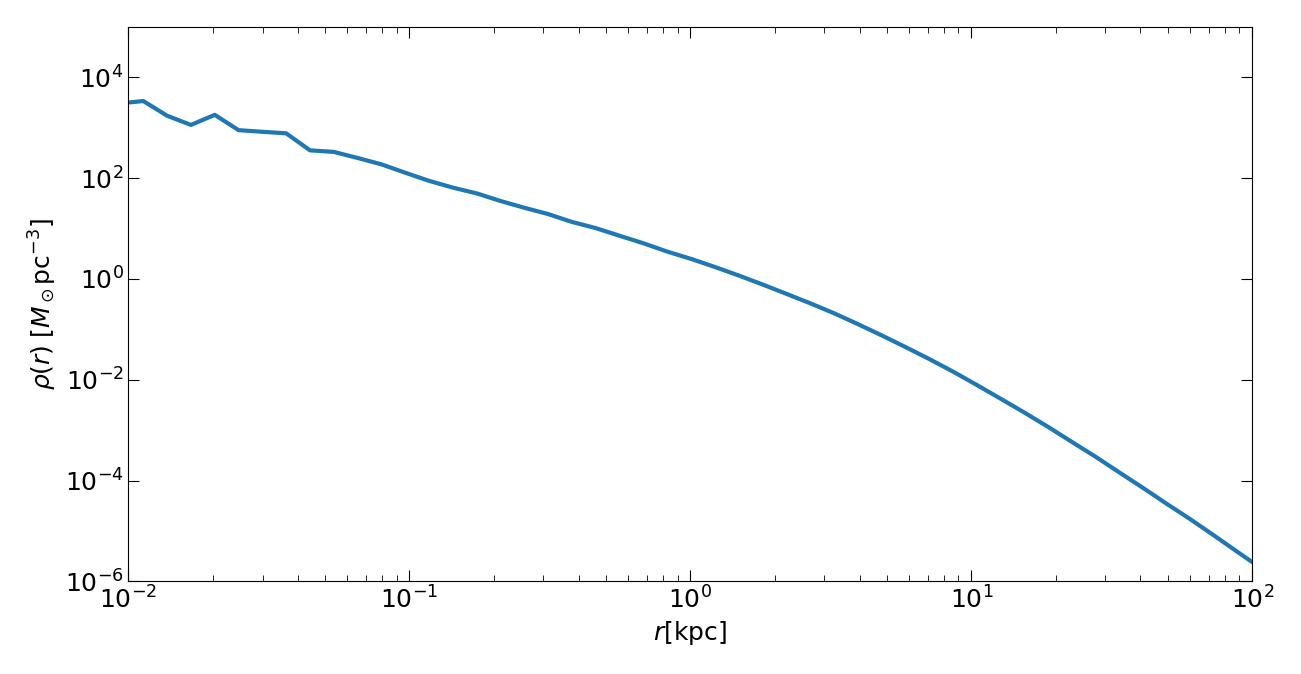
\includegraphics[width=\textwidth]{IC.png}
	\caption{An example of the mass density profile of the progenitor galaxies. The initial conditions for the profile in question were the same as in table \ref{table:properties}; with the exception of the number of dark matter and stellar particles, which were only $10\%$ of their respective values. The noise in the left-side of the profile is caused by this low particle sample.}
	\label{figure:IC_density_profile}
\end{figure}

The seven merger simulations thus comprise of mergers of two identical progenitor galaxies with properties described in table \ref{table:properties}. These galaxies are merged on a nearly parabolic orbit with an initial separation of $d = 30 \; \mathrm{kpc}$. This kind of orbit makes the approach of the galaxies swift, and causes the stellar cusps to merge before $t \sim 300 \; \mathrm{Myr}$.

The simulation data that I will be analysing, comes in the form of snapshots of the merger remnants. These snapshots are taken at the simulation time of $\sim 2 \mathrm{Gyr}$. At this point the progenitor galaxies have merged into a single merger remnant, however, their central SMBHs have not yet merged and still exist in the form of a central binary. The snapshots contain the positions, velocities and masses of every particle.

\section{Core Size Measurements}

In order to test if a galaxy is cored, I calculate its surface brightness profile and check if the centre of the galaxy contains a light deficit.

The surface brightness profiles are calculated from the merger remnant snapshots using the following procedure. First, the coordinate system is changed to centre-of-mass coordinates, and the stellar particles are projected onto a 2D plane. Next, the mass inside logarithmically spaced radial bins is calculated, resulting in a radial surface mass density profile. This is repeated 100 times from random viewing angles, which naturally results in 100 slightly different density profile projections. These profiles are then averaged azimuthally, which results in a smooth surface mass density profile. Finally, by assuming a mass-to-light ratio for the stellar particles, the surface mass density profile can be turned into a surface brightness profile \citep{Rantala2018}. 

Determining the mass-to-light ratios of the stellar particles in the simulated merger remnants is problematic, as the simulations do not contain information about their ages and metallicities. The only properties that the stellar particles have are their position, velocity, and a mass that is identical for all of them. These are not enough to make valid, physically accurate, assumptions on their specific mass-to-light ratios. For this reason, a constant mass-to-light ratio of $M/L = 4$ is used. This is equivalent to the ratio derived from dynamical modelling of NGC 1600 by \cite{Thomas2016}. Thus, the use of this particular $M/L$ in the analysis of the simulation results, fits in well with the already established desire of similarity between the physical properties of the simulated merger remnants and NGC 1600.

Figure \ref{figure:surface_brightness} shows the surface brightness profiles of every simulated merger remnant. Studying the curves, one can already see that the presence of central SMBHs in the merger progenitors causes a clear brightness deficit near the centre of the merger remnant. In addition, there is a systematic effect that shows a clear positive correlation, between the mass of the black hole binary and the amount of missing light in the core.

\begin{figure}
	\centering
	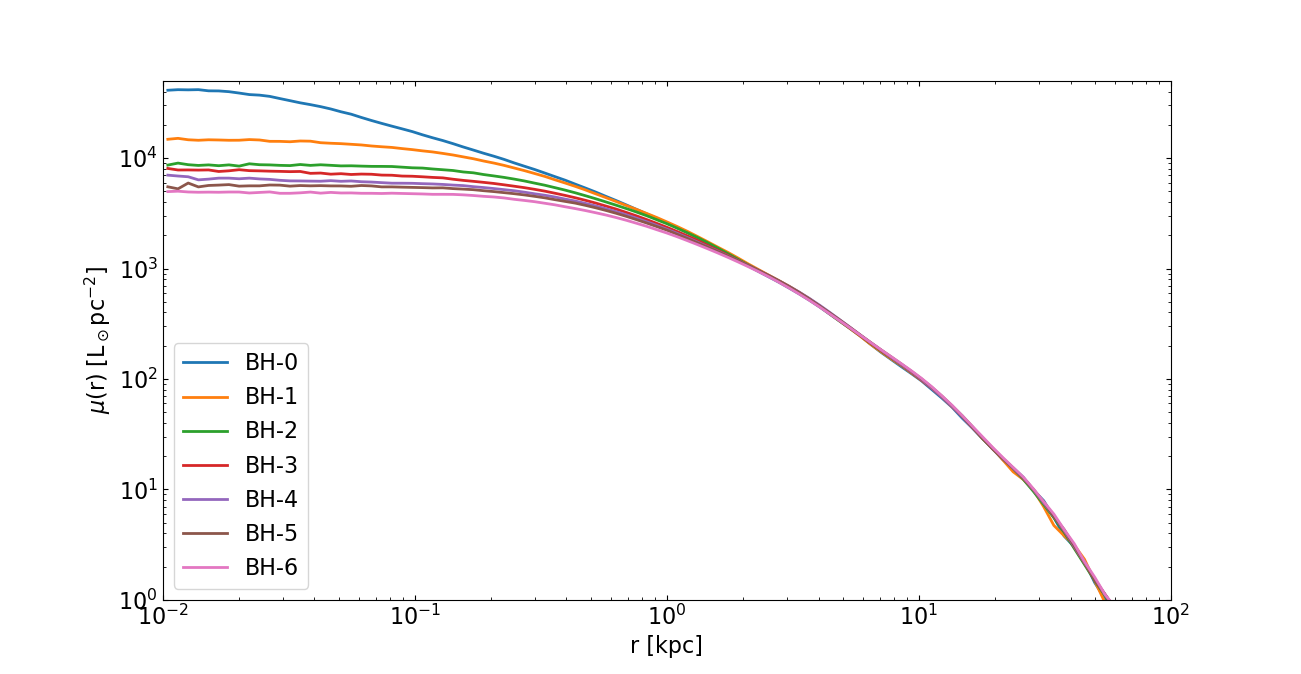
\includegraphics[width=\textwidth]{SurfaceBrightnessProfiles.png}
	\caption{Surface brightness profiles from every simulated merger remnant. These were calculated by dividing the stellar particles in the simulated galaxy remnants into 100 radial logarithmic bins, and averaging the surface brightnesses inside these bins through 100 random viewing angles. The luminosity of the particles was estimated by assuming a constant mass-to-light ratio of $M/L = 4$.}
	\label{figure:surface_brightness}
\end{figure}

The lack of light in the surface brightness profiles reveals the presence of cores; however, determining the precise sizes of the cores requires knowledge of the exact locations where the profiles start to deviate from a Sérsic-profile fit (see section \ref{section:core_galaxies} for further discussion). The core radii in the merger remnants are calculated by using the "Levenberg-Marquardt" fitting algorithm, to fit both a core-Sérsic model (equation \ref{eq:core-sersic}) and a Nuker model (equation \ref{eq:nuker}) to their surface brightness profiles. For the most part, the initial guesses used for the values of the fitting parameters in the fitting algorithm, were determined through trial-and-error, as well as knowledge of their likely order of magnitude. This was not the case for the Sérsic-index ($n$) in the core-Sérsic profile however. In order to reduce degeneracy between the fitting parameters, $n$ was fixed to $n=4$ for all core-Sérsic profile fits.

\begin{figure}
	\centering
	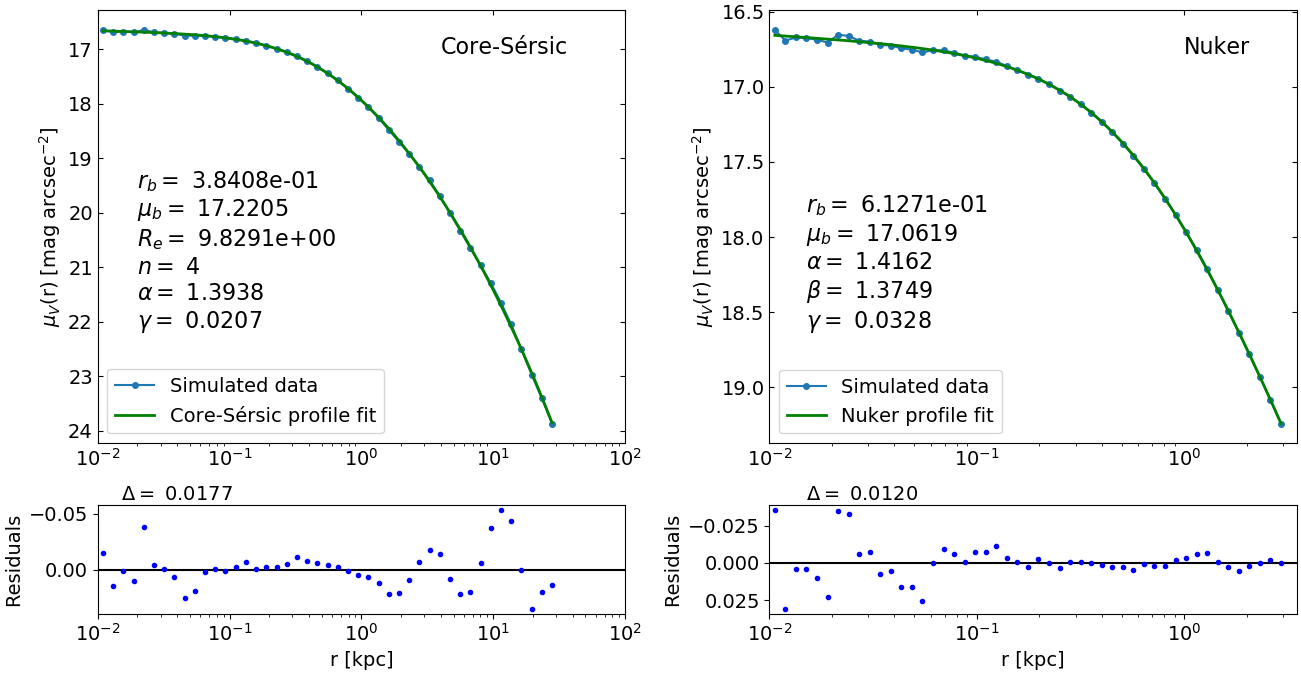
\includegraphics[width=\textwidth]{core_nuker_fits.png}
	\caption{Core-Sérsic and Nuker profile fits of surface brightness profiles calculated from the BH-3 merger remnant (left and right figures, respectively). The best-fit parameters are shown on the figures and are in the same units as the axes (i.e. $r_b$ and $R_e$ in $\mathrm{kpc}$, and $\mu_b$ in $\mathrm{mag \; arcsec^{-2}}$, where $\mathrm{mag}$ denotes V-band magnitudes). The relative residuals of the fits are plotted under their respective figures. The $\Delta$-parameter shows the root-mean-square of the residuals.}
	\label{figure:core_nuker}
\end{figure}

Figure \ref{figure:core_nuker} shows a comparison between the core-Sérsic and Nuker profile fits for the BH-3 merger, while figures \ref{figure:all_core} and \ref{figure:all_nuker} show these fits for every simulated remnant containing an SMBH binary. The values of the best-fit parameters are shown on the figures. The units of the surface brightness are changed from $L_\odot \; \mathrm{pc^{-2}}$ to $\mathrm{mag \; arcsec^{-2}}$ (where $\mathrm{mag}$ is the magnitude in the V-band) using the common conversion formula:
\begin{equation}
\mu = M_\odot + 21.572 - 2.5 \log(I), 
\end{equation}
where $M_\odot$ is the absolute magnitude of the Sun in a specific spectral band (in our case the V-band magnitude of $4.83$ is used), and $I$ is the surface brightness in $L_\odot \mathrm{pc^{-2}}$. The relative residuals of the fits are plotted under their respective surface brightness profiles.

The root-mean-square of the relative residuals of the fits, are comparable to the values seen in profile fits of observed surface brightness profiles: $\Delta \approx 0.02 \; \mathrm{mag \; arcsec^{-2}}$ \citep{Dullo2012}. However, while the RMS of the residuals show that the fits describe the surface brightness profiles rather well, most of the fits have somewhat large residual scatter near the centre of the merger remnant. This scatter is especially noticeable in the Nuker fits, since in order to get sensible values for the fitting parameters, the fitting range needs to be concentrated in the galactic centre (in this analysis, the fitting range used for the Nuker profile was $\sim 0.04 - 3 \; \mathrm{kpc}$, which is an order of magnitude lower compared to the range used for the core-Sérsic fit $\sim 0.04 - 60 \; \mathrm{kpc}$). 

The larger central residual scatter is most likely not indicative of any kind of significant physical structure in the merger remnant cores, but simply a result of the logarithmic spacing of the bins in the surface brightness profiles. The bins near the centre inherently contain less particles than the outer bins. When calculating the 100 projected surface brightness profiles from random viewing angles, this causes the variations in binned luminosities to be larger in the central bins, resulting in a final averaged profile that contains small jumps as well as small dips in its central luminosity. These arbitrary inconsistencies naturally cause the residuals of the fits to be scattered in a random way near the centre of the simulated galaxy. Unfortunately, remedying this problem by using bins that have a constant number of particles did not yield satisfactory results, due to the total number of particles being extremely small near the centre.

Interestingly, all of the core-Sérsic fits show a peak in the size of the residuals at around $\sim 10 \; \mathrm{kpc}$. Once again, this residual property is probably just a small anomaly in the simulations and not indicative of any physical structure that could be found in actual merger remnants. However, the fact that this residual anomaly appears in the surface brightness profile of every simulation, indicates that; even though the masses of the SMBHs in the merger progenitors have a large effect on the central regions of the merger remnant, the outer regions are left relatively unaffected. In fact, the central SMBH binary is only expected to affect the outer regions of the merger remnant, through stellar particles that have been ejected from the galactic centre. 

All of the significant residual variations between the profile fits of the simulated merger remnant galaxies are concentrated near their respective centres. This implies that the results of the different simulations vary significantly from each other only due to the formation of a central SMBH binary, since the similar shapes of the outer regions of the residual plots can be explained through the limited range of the gravitational spheres-of-influence (SOI) of the binaries. The 2D projected radii of the SOI of the simulated SMBH binaries can be seen in table \ref{table:s-o-i}. These radii were calculated by, finding the radius of a sphere (centred at the centre-of-mass of the host galaxy) that contains the amount of stellar mass equivalent to the mass of the SMBH binary. The projected sizes of the radii were determined through a similar relation to the one described in equation \ref{eq:projection_approximation}.


\begin{table}
	\begin{center}
		\begin{tabular}{| c | c |}
		\hline
		Simulation & $r_\mathrm{SOI}$ $\mathrm{[kpc]}$ \\
		\hline
		BH-1 merger & 0.143 \\
		BH-2 merger & 0.256 \\
		BH-3 merger & 0.394 \\
		BH-4 merger & 0.515 \\
		BH-5 merger & 0.620 \\
		BH-6 merger & 0.757 \\
		\hline
		\end{tabular}
	\end{center}
	\caption{Estimations of the projected radii of the spheres-of-influence ($r_\mathrm{SOI}$) for every simulated SMBH binary. These were calculated by finding the radius of a sphere, that contains the amount of stellar mass equivalent to the mass of the binary, inside its host merger remnant. The 2D projections of the radii were determined by using a relation, similar to the one described in equation \ref{eq:projection_approximation}.}
	\label{table:s-o-i}
\end{table}

\begin{figure}
	\centering
	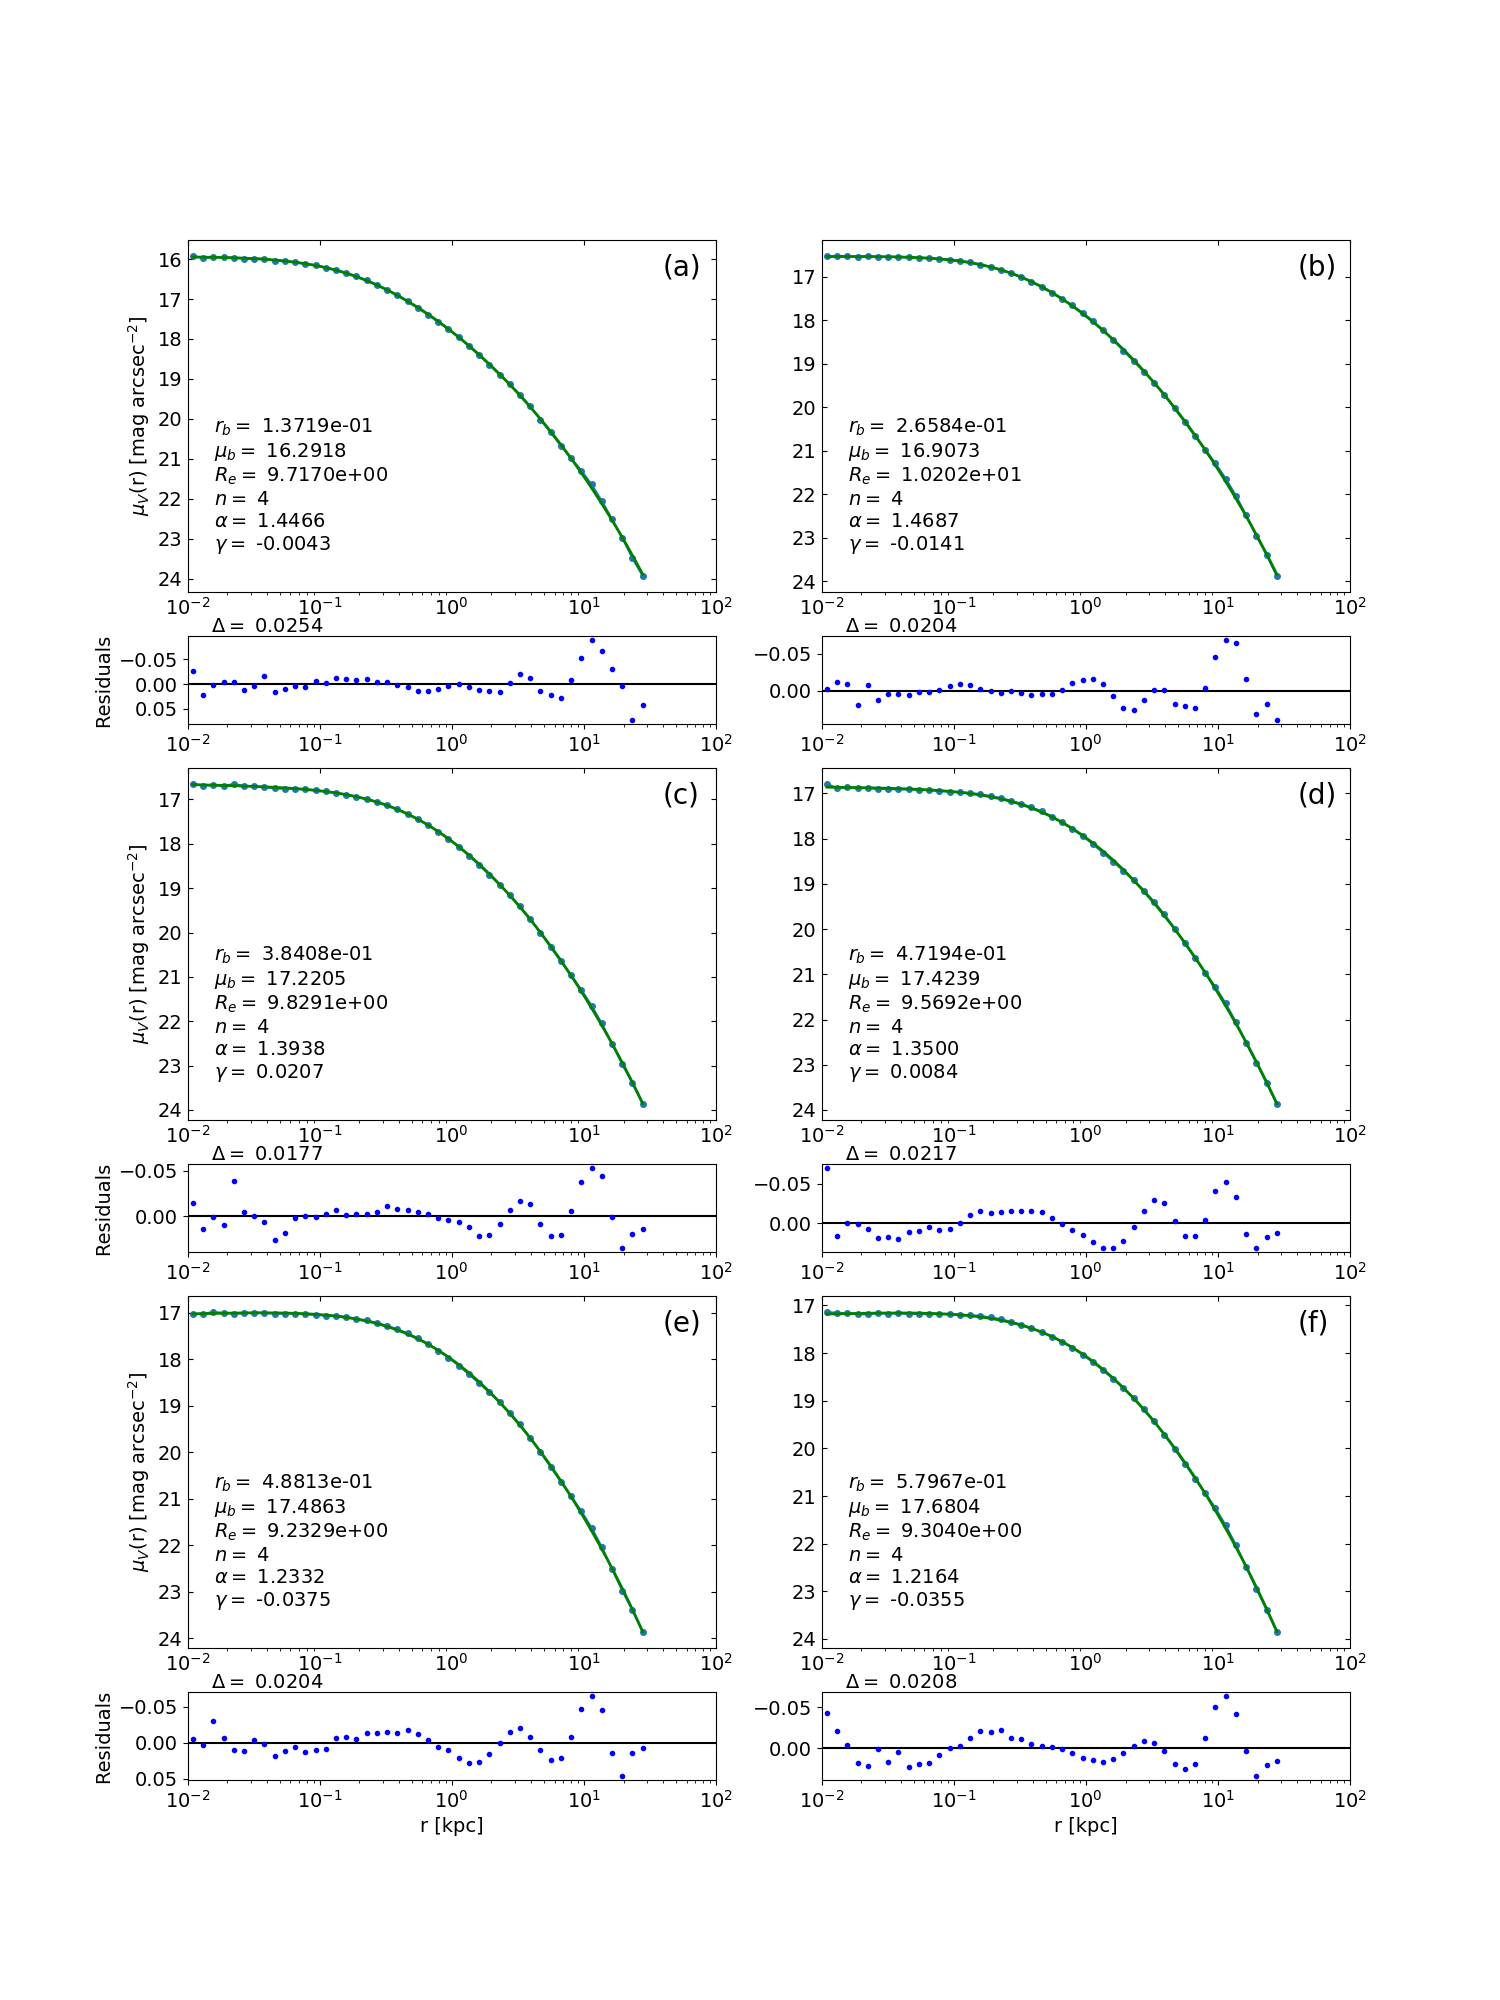
\includegraphics[width=\textwidth]{all_core_profiles.png}
	\caption{Core-Sérsic profile fits for the binned surface brightness profiles of all of the individual simulated merger remnants, that had progenitors containing central supermassive black holes. The letters (a)-(f) denote the different snapshots ((a): BH-1 merger, (b): BH-2 merger, (c): BH-3 merger, (d): BH-4 merger, (e): BH-5 merger, (f): BH-6 merger).}
	\label{figure:all_core}
\end{figure}

\begin{figure}
	\centering
	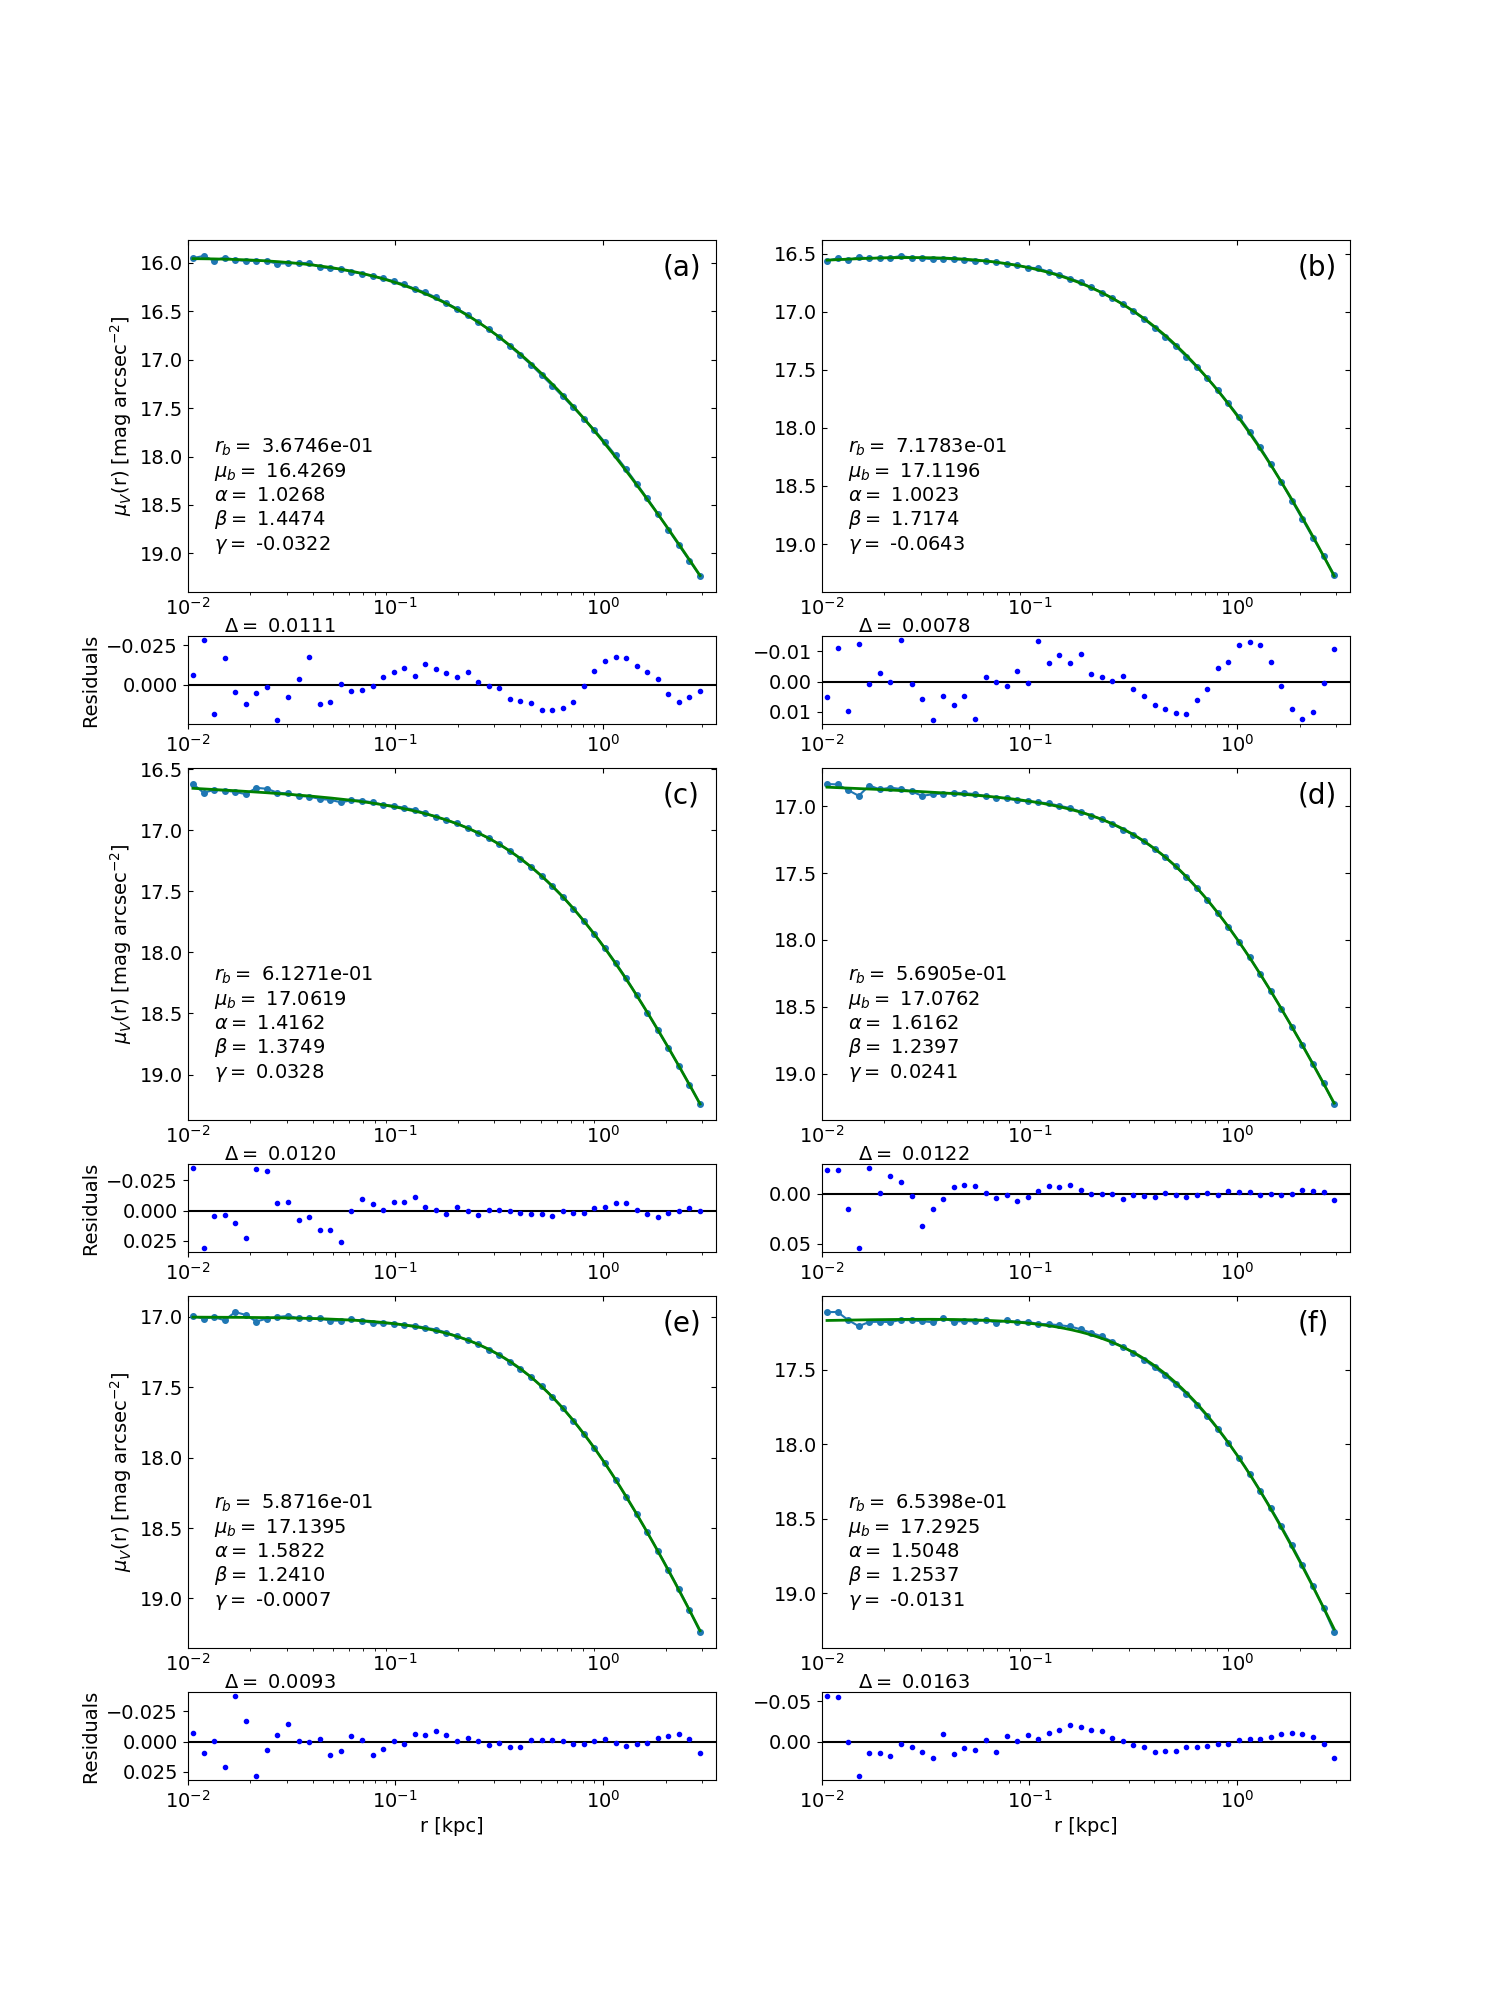
\includegraphics[width=\textwidth]{all_nuker_profiles.png}
	\caption{Nuker profile fits for the binned surface brightness profiles of all of the individual simulated merger remnants, that had progenitors containing central supermassive black holes. The letters (a)-(f) denote the different merger remnants ((a): BH-1 merger, (b): BH-2 merger, (c): BH-3 merger, (d): BH-4 merger, (e): BH-5 merger, (f): BH-6 merger).}
	\label{figure:all_nuker}
\end{figure}

Figures \ref{figure:all_core} and \ref{figure:all_nuker} show that the value of the core radius estimate depends quite strongly on which model was used. Which of the values is more representative of the actual core radius is not certain, as whether the core-Sérsic or the Nuker model is better at estimating the size of the core is still a matter of debate \citep{Lauer2007, Dullo2012}. While the RMS of the relative residuals seems to be consistently (although just marginally) smaller when using the Nuker model, its best-fit value for $r_b$ has been found to be strongly dependent on the fitting range \citep{Graham2003}. Furthermore, in order to get sensible values for every parameter of the Nuker model, its fitting range has to be narrowed down closer to the galactic centre. An example of a parameter that requires such a fitting range is the $\alpha$-parameter. Using similar fitting ranges to the ones used in this thesis, \cite{Rantala2018} find that, when trying to fit the Nuker model over the same radial range as the core-Sérsic model, the paramter in question gets values of $\alpha \lesssim 1$, which as \cite{Graham2003} explain, may prevent the model from describing the profile as a combination of two power-laws. The dependence that the Nuker model parameters have on the fitting range, implies that its core radius estimates can be inconsistent. Similar fitting range dependencies are not observed in the core-Sérsic model.

In addition to the core radii derived through model fitting, I analyse a third estimate for the size of the core, by calculating the cusp radius $r_\gamma$ (see section \ref{section:core_galaxies} for the explanation of the cusp radius) for all of the merger remnants with central SMBH binaries (BH-1 - BH-6 mergers). These are derived by determining the gradient of the surface brightness profiles, and using a function minimization algorithm \citep{NelderMead} to minimize the difference $\big| \frac{d\mu(r)}{dr} - \left( - \frac{1}{2} \right) \big|$. This shows the location where the gradient gets the value $-1/2$, which corresponds to the cusp radius. 

\begin{figure}
	\centering
	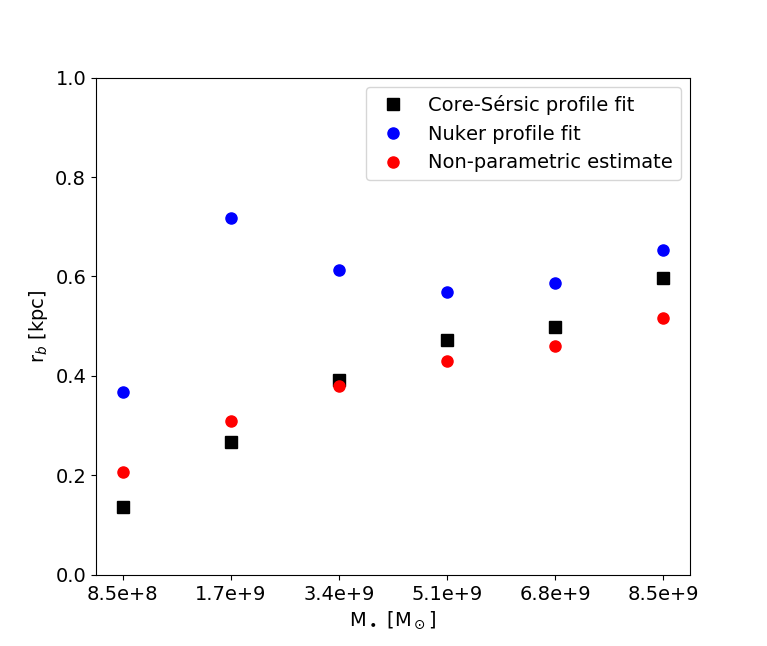
\includegraphics[width=\textwidth]{rb_mass_relation.png}
	\caption{Comparison of the different core radius estimates of the merger remnants. These estimates were derived through three different methods: Core-Sérsic profile fitting (black squares), Nuker profile fitting (blue circles) and  finding the "cusp radius" (red circles). The x-axis shows the masses of the central SMBH binaries in the merger remnants.}
	\label{figure:radii_comparison}
\end{figure}

Figure \ref{figure:radii_comparison} compares the core radius estimates derived using each of the three methods, for every simulated merger remnant with an SMBH binary. From the figure, a clear positive correlation between the size of the core and the binary mass can be observed. However, the break radii from the Nuker fits are consistently larger than the other core radius estimates. They also have, in general, the largest deviations from the other core radii, and even contain two values that seem to break the trend of the core radius growing with the central SMBH binary mass (these being the break radii for the BH-2 and BH-3 mergers). Similar larger-than-expected Nuker core radii can be seen in the analysis of the same simulations by \cite{Rantala2018}. Like in figure \ref{figure:radii_comparison}, the difference in the Nuker break radii and the other core radius estimates for the two mergers with the smallest and third smallest central SMBH binaries, are significantly larger than for the other mergers. The fact that these large deviations are present in both this analysis and the analysis by \cite{Rantala2018}, further implies that, due to its high dependence on the fitting range, the Nuker model sometimes provides inconsistent values for the break radius.

The fact that the size of the core is dependent on the mass of the central SMBH binary, is clear evidence towards the cores being formed through a scouring process by the binary black holes. Binaries with larger masses have larger gravitational spheres-of-influence (table \ref{table:s-o-i}), which naturally leads to the ejection of stellar particles that orbit farther away from the galactic centre (the larger SMBH binary mass also causes the stellar material to be ejected at a larger velocity). 

This positive correlation between the core size and the SMBH binary mass has also been identified in independent measurements of the break radius and the central SMBH mass in cored galaxies \citep[e.g.][]{deRuiter2005, Lauer2007Cusp, Thomas2016}. The fact that this effect can be seen, not only in the simulations, but also in observations, makes it clear that merging SMBH binaries are a likely source for the observed cores.

Alongside the size of the core, the surface brightness deficit also becomes larger as the central SMBH binary mass grows (figure \ref{figure:surface_brightness}). This can be explained trough the concept of the loss-cone. The condition that defines the loss-cone (equation \ref{eq:loss-cone}) shows, that the maximum angular momentum at which a star can interact strongly with the binary, grows alongside the binary mass. This means that, a larger SMBH binary mass causes more of the orbiting stellar particles to be located in the strong interaction range. Not only does the loss-cone widen, but the maximum velocities at which a stellar particle can interact strongly with the binary, also become larger. Thus, a more massive central SMBH binary naturally results in the ejection of a larger number of stellar particles, leading to a larger central surface brightness deficit.  

\section{Velocity Anisotropy}

%\begin{figure}[h]
%	\centering
%	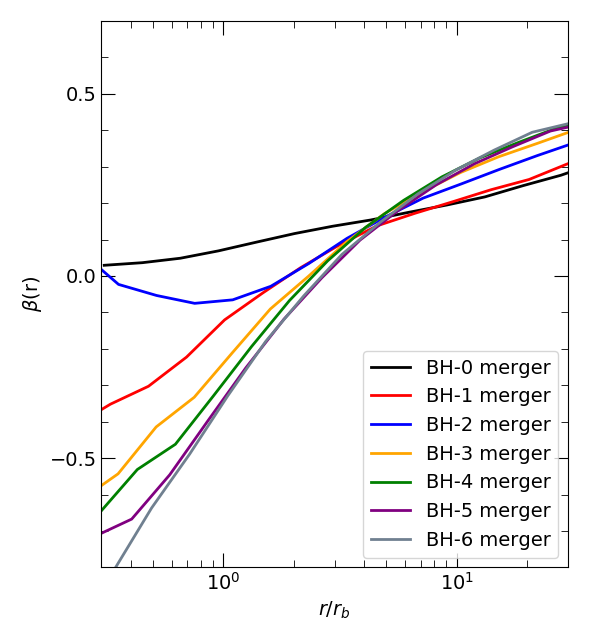
\includegraphics[width=0.9\textwidth]{beta.png}
%	\caption{Velocity anisotropy (beta) profiles of the simulated merger remnants with central black holes.}
%\end{figure}

Another method of determining whether the low-luminosity core of a galaxy is formed through a scouring process by binary black holes, is to study the velocity anisotropy profile. \cite{BinneyTremaine} define this profile as:
\begin{equation}
\beta(r) = 1 - \frac{\sigma_\theta^2 + \sigma_\phi^2}{2\sigma_r^2} = 1 - \frac{\sigma_t^2}{\sigma_r^2}, \label{eq:beta}
\end{equation}
where $\sigma_\theta$, $\sigma_\phi$ and $\sigma_r$ are one-dimensional velocity dispersions in the spherical coordinates, and $\sigma_t = \sqrt{(\sigma_\theta^2 + \sigma_\phi^2) / 2}$ is the tangential velocity dispersion. This $\beta$-parameter describes the ratio of tangential velocity dispersion in the stellar system to the radial velocity dispersion. As such, it provides information about the nature of the stellar orbits around the black hole binary. A negative value for $\beta$ shows an abundance of tangential orbits, whereas a positive $\beta$ corresponds to an abundance of radial orbits. 

Figure \ref{figure:beta_no_rb} shows $\beta$-profiles calculated from all of simulated merger remnants using equation \ref{eq:beta}. In order to get the velocity dispersions, the stellar particles in the remnant galaxies were first divided into logarithmic bins, and their velocities were changed from a Cartesian to a spherical coordinate system. Next, the root-mean-squares, which correspond to the velocity dispersions, of the different spherical velocity components were calculated for each bin separately, resulting in a $\beta$-value for every bin. Plotting these values gives the profiles in figure \ref{figure:beta_no_rb}. 

\begin{figure}
	\centering
	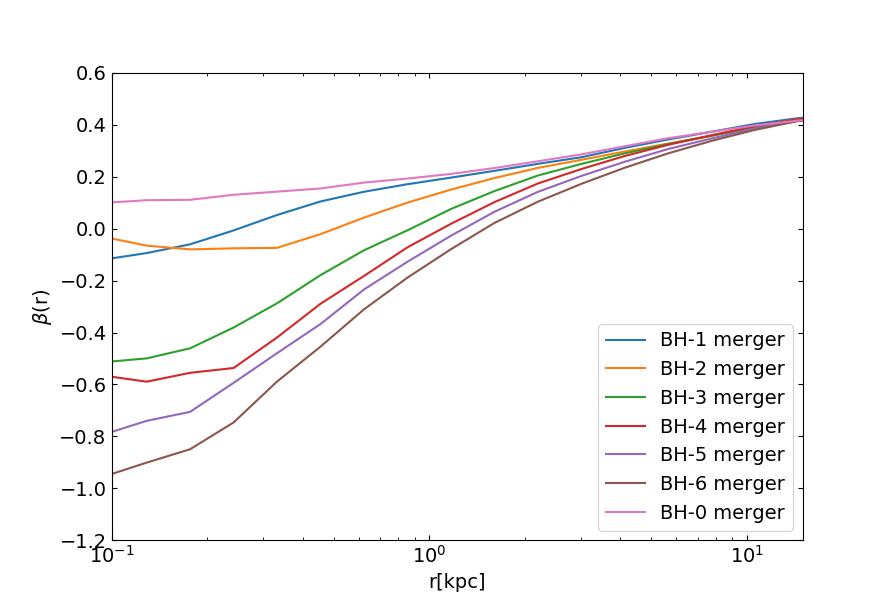
\includegraphics[width=0.9\textwidth]{beta_no_rb.png}
	\caption{Velocity anisotropy ($\beta$) profiles for every simulated merger remnant. The profiles are calculated from the velocity dispersions in radial logarithmic bins, using equation \ref{eq:beta}. Comparing the outer regions to the central regions of the merger remnants, the profiles of show that the former is radially dominated, while the latter tangentially dominated.}
	\label{figure:beta_no_rb}
\end{figure}

According to the $\beta$-profiles, the outer areas of the remnants are dominated by radial orbits (positive $\beta$), while the majority of orbits near the centre are tangential (negative $\beta$). As the initial merger progenitors used in the simulations contained isotropic $\beta$-profiles ($\beta = 0$), an area with negative $\beta$ would imply that the stars on radial orbits have been lost from that part of the system. It has been shown that hardening black hole binaries can eject stars on highly radial orbits from the galactic core, which results in the central region becoming dominated by mostly tangential orbits (and thus a negative $\beta$). The ejected stars can then, in turn, cause the outer orbits to become more radial \citep{Quinlan1997, Milosavljevic2001, Thomas2014}, which would explain why the $\beta$-profiles are not isotropic in the outer regions of the merger remnants.

Figure \ref{figure:beta_no_rb} clearly shows that the presence of an SMBH binary has an effect on the shape of the $\beta$-profiles. Not only is the slope of the profile steeper for merger remnants that contain a more massive central SMBH binary, but the only merger with a profile that is completely dominated by radial velocity dispersion, is the one which does not contain black holes (the BH-0 merger). The correlation between the shapes of these profiles and the mass of the central black hole binary, makes sense in the context of ejection of stellar particles. The larger the mass of the SMBH binary, the larger its gravitational sphere-of-influence. This results in radially orbiting stellar particles being able to be ejected farther away from the galactic centre. Furthermore, the larger binary mass strengthens widens the loss-cone regime, allowing for the ejection of radially orbiting stellar particles with faster orbital velocities. This naturally leads to the $\beta$-profiles to be,in general, more negative

\begin{figure}
	\centering
	\begin{subfigure}[b]{0.39\textwidth}
		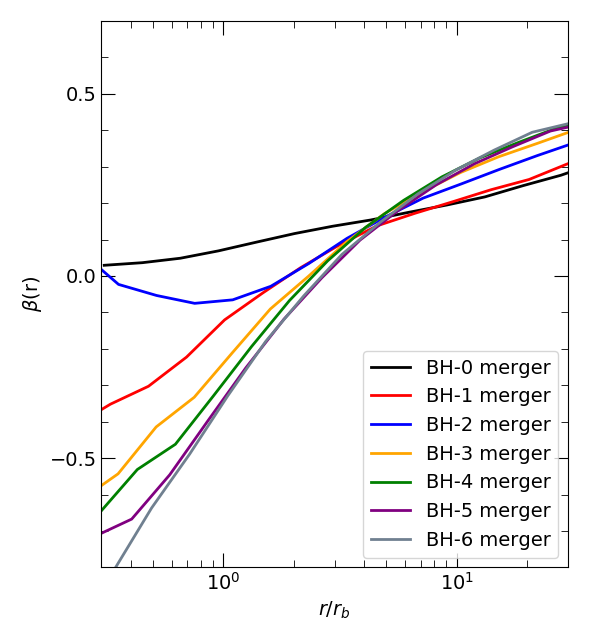
\includegraphics[width=\textwidth]{beta.png}	
		\caption{Simulated merger remnants}
	\end{subfigure}
	\begin{subfigure}[b]{0.60\textwidth}
		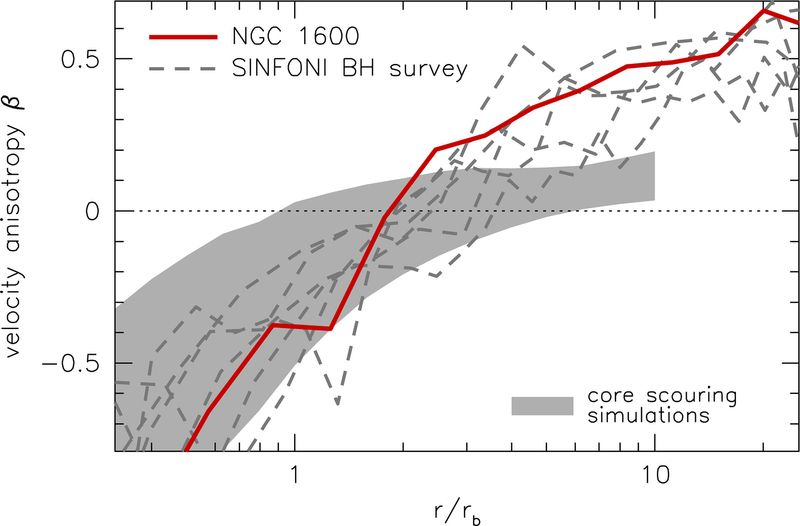
\includegraphics[width=\textwidth]{thomas2016.jpg}
		\caption{NGC 1600}
	\end{subfigure}
	\caption{(a): The $\beta$-profiles of the simulated merger remnants as a function of distance from the centre, scaled by their respective break radius. For the merger remnant without a core (BH-0), the value used for the break radius is $r_b = 1 \; \mathrm{kpc}$. The profile for the BH-2 merger shows an increase in the value of $\beta$ near the centre of the merger remnant, which is simply the same increase seen in figure \ref{figure:beta_no_rb}, amplified by the break radius scaling. (b): $\beta$-profile of NGC 1600, alongside profiles of galaxies from the SINFONI black hole survey \citep{Saglia2016} and the range of possible anisotropies found in N-body simulations of the core scouring mechanism \citep{Thomas2016}.}
	\label{figure:beta_NGC1600_Simul}
\end{figure}

Figure \ref{figure:beta_NGC1600_Simul} shows both the observed $\beta$-profile of NGC 1600, and the profiles from the simulated merger remnants. The profiles in the figure are scaled by the core radius of the respective galaxy. Even by eye, it can clearly be seen that both the simulated $\beta$-profiles and the observed profile of NGC 1600, are similar to each other (not counting the anomalous profile for the BH-2 merger). However, looking closely at the values on the axes of both plots, the observed NGC 1600 profile seems to be slightly steeper compared to the simulated profiles, having a more tangentially dominated inner profile and a more radially dominated outer profile. 

%According to \cite{Rantala2018} it is likely that, the larger steepness of the profile seen in NGC 1600 is due the simulations only comprising a single generation of completely isotropic ($\beta = 0$) mergers. Most observed cored galaxies, including NGC 1600, are most likely the result of multiple generations of mergers. The progenitors of the observed major merger remnant galaxy would thus have already had tangentially biased $\beta$-profiles, leading to a remnant with an even steeper profile.

According to \cite{Rantala2018}, the kinematics being more tangential close to the core in NGC 1600 when compared to the simulations, could be caused by further adiabatic growth of its central SMBH mass. \cite{Young1980} shows that black holes that grow adiabatically through, for example accretion of gas, can cause the surrounding stellar orbits to become more tangential. If the time scale of the mass growth is smaller than the relaxation time scale of the galaxy, while also being larger than the dynamical time scale of the whole stellar system, the growth can be considered adiabatic. This results in the conservation of both the angular momentum and the radial action of the stellar orbits (radial action being one of the momenta in the canonical Hamiltonian coordinates called \textit{angle-action variables}; \citealt{BinneyTremaine}), which, due to the now higher gravitational potential induced by the central black hole, causes the orbits to become more circular. Although this effect is not strong enough to account for the entire shape of the $\beta$-profile \citep{Thomas2016}, it could certainly be a reason for the more tangentially dominated core regions seen in the observations.

As for the outer region of the $\beta$-profile of NGC 1600, it is possible, that the reason why it is more radially dominated than the outer parts of any of the simulated merger remnants, is due to the lack of minor-mergers in the simulations \citep{Rantala2018}. These minor-mergers would deposit all of their mass in the outer regions of the galaxy, and would thus disrupt only the outer stellar orbits, making some of them more radial. Furthermore, minor mergers would not contribute to the destruction of radial orbits near the centre of the galaxy, as the smaller progenitor galaxy would not contain a central SMBH.

\section{Line-of-Sight Kinematics}

\subsection{2D Kinematic Maps}

In order to make sure that the KETJU simulations produce results that are in agreement with observations, I also analyse the line-of-sight (LOS) kinematics of the simulated merger remnants. The analysis is focused on the four different LOS velocity distribution (LOSVD) parameters: the average LOS velocity $V_\mathrm{avg}$, the velocity dispersion $\sigma$, and the $h_3$ and $h_4$ parameters (see section \ref{section:IFU}). 

The above LOSVD-properties are calculated using a Python-script (Matteo Frigo, internal communication), which makes use of the Voronoi tessellation algorithm by \cite{Cappellari2003}. It provides binned statistics of the LOS velocities, and forms 2D kinematic maps similar to ones provided by integral-field units (IFU-maps), in order to help visualise the LOSVD properties. First, when using the script, the "line-of-sight" is defined as the intermediate axis of the merger remnant, after which a 2D line-of-sight projection of the remnant is produced, by orienting it accordingly using the inertia tensor. The 2D projection is then divided into "spaxels" using the aforementioned Voronoi tessellation algorithm. The shape and size of the spaxels are determined so that each one contains the same signal-to-noise ratio, which in our simulated case is defined as the number of stellar particles. The LOS-velocities inside the spaxels are then made into a histogram, into which the modified Gaussian function (equation \ref{eq:mod_gaussian}) is fitted. This gives the values of the LOSVD parameters: $V_\mathrm{avg}$, $\sigma$, $h_3$ and $h_4$ for the spaxel in question. Finally, the values of the spaxels are plotted, resulting in 2D Voronoi-binned IFU-maps of all of the four parameters.

Figure \ref{figure:IFU-maps} shows the Voronoi-binned 2D maps of the four LOS velocity distribution parameters for the simulated BH-0 merger (no central SMBH) and the BH-6 merger (largest central SMBH), as well as for two observed galaxies NGC 3414 and NGC 4111, which are known slow and fast rotators, respectively. The contours, which are added to help visualise the shape of the galaxy, denote flux isophotes of the merger remnants, and have a spacing of one magnitude. Similar maps for the rest of the simulated merger remnants can be seen in figure \ref{figure:rest_of_voronoi}.

The IFU-maps in figures \ref{figure:IFU-maps} and \ref{figure:rest_of_voronoi} show that the average LOS velocities of the simulated merger remnants are far from isotropic, with most of the remnants that contain central binary SMBHs showcasing KDCs. Some of the simulated remnants (BH-4 - BH-6 mergers) even contain a clear counter rotating structure inside the KDC \citep{Rantala2019}. Curiously, the map for the BH-2 merger does not seem to contain any significant features. What causes this discrepancy is uncertain. However, the features seen in the maps of the other remnants, alongside the relatively low average LOS-velocities in all maps, imply that all of the merger remnants are likely slow rotators. Since slow rotator galaxies are assumed have been formed through gas-poor "dry" mergers, not unlike core galaxies, this is result is somewhat expected.

\begin{figure}
	\centering
	\begin{subfigure}[b]{0.49\textwidth}
		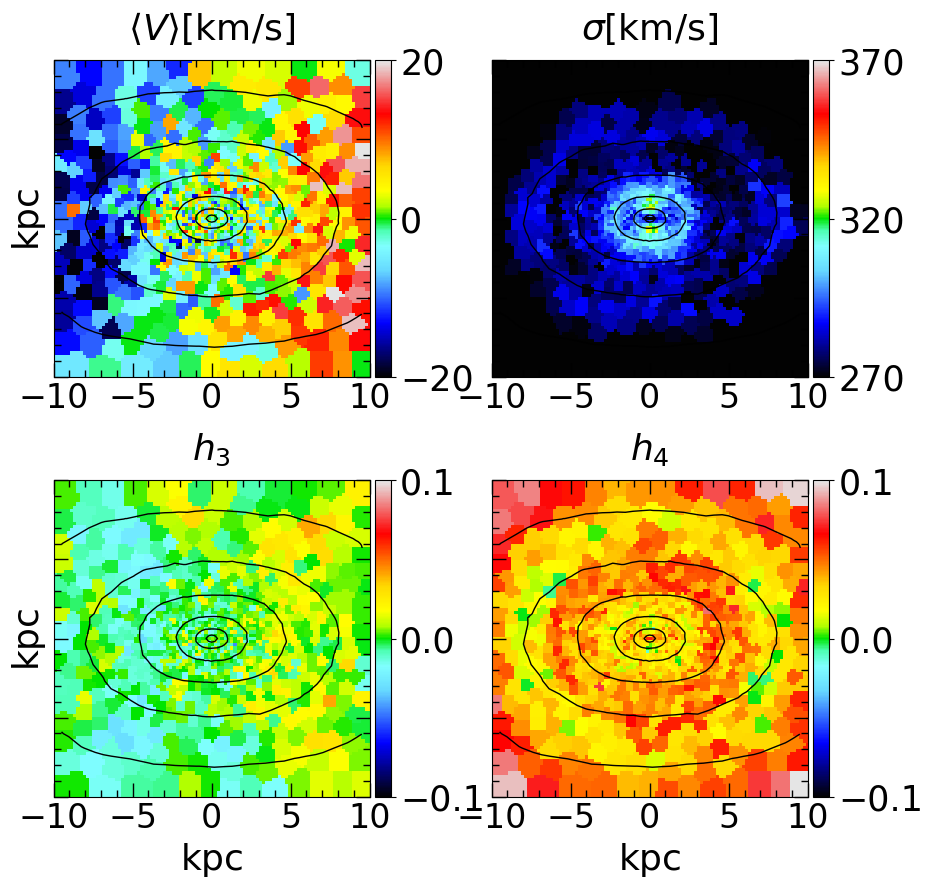
\includegraphics[width=\textwidth]{BH_0.png}
		\caption{BH-0 merger remnant}
	\end{subfigure}
	\begin{subfigure}[b]{0.49\textwidth}
		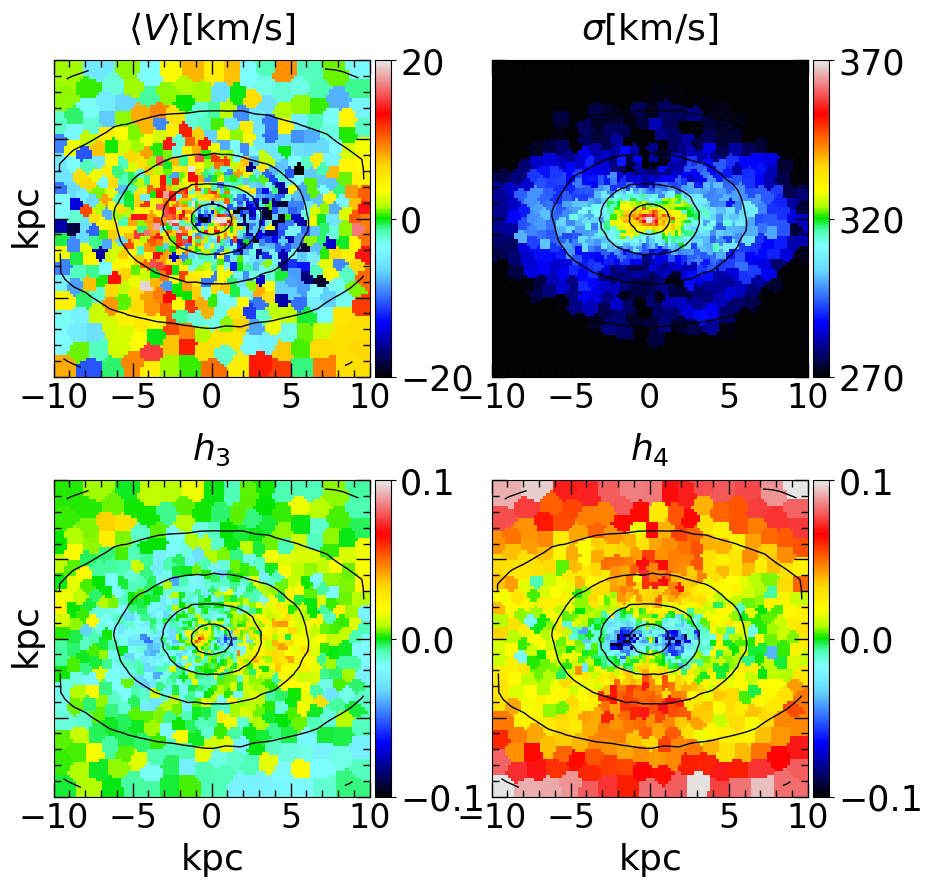
\includegraphics[width=\textwidth]{BH_6.png}
		\caption{BH-6 merger remnant}
	\end{subfigure}
	\begin{subfigure}[b]{0.49\textwidth}
		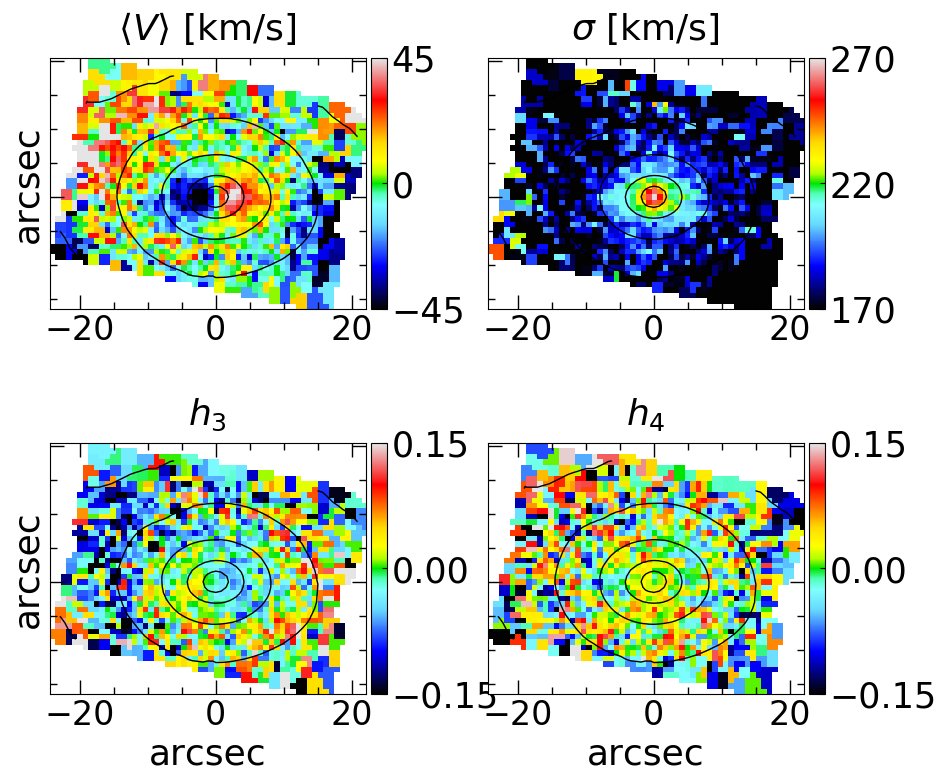
\includegraphics[width=\textwidth]{NGC3414_r6_voronoi.png}
		\caption{NGC 3414}
	\end{subfigure}
	\begin{subfigure}[b]{0.49\textwidth}
		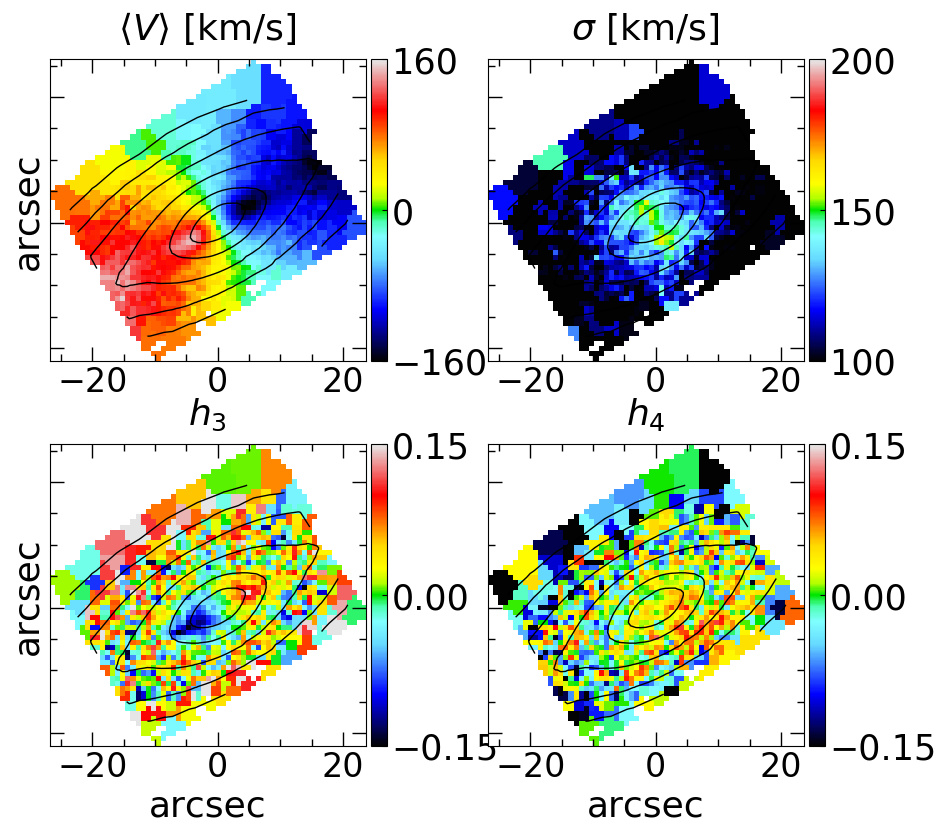
\includegraphics[width=\textwidth]{NGC4111_r1_voronoi.png}
		\caption{NGC 4111}
	\end{subfigure}
	\caption{IFU-maps of average LOS-velocities, velocity dispersion, $h_3$ parameters and $h_4$ parameters from two simulated merger remnants and two observed galaxies. The four maps in figure (a) are from the BH-0 merger, and the four in figure (b) are the BH-6 merger. Figures (c) and (d) show IFU-maps of known slow (NGC 3414) and fast rotator (NGC 4111) galaxies from the $\mathrm{ATLAS^{3D}}$ survey \citep{Emsellem2004, Cappellari2011, Krajnovic2011}.}
	\label{figure:IFU-maps}
\end{figure}

The velocity dispersion maps in figures \ref{figure:IFU-maps} and \ref{figure:rest_of_voronoi} show a clear connection between the mass of the central SMBH binary and the velocity dispersion at the centre of the galaxy. The presence of an SMBH binary causes the formation of a central velocity dispersion peak in the $\sigma$-distribution, the strength of which correlates positively with the mass of the binary. Furthermore, as the mass of the SMBH binary grows, the size of the area with the highest velocity dispersion in the galaxy also grows. Additionally, the growing binary mass seems to cause the high-$\sigma$ area to get more and more aligned with the major-axis of the galaxy. Most of these effects can easily be identified when comparing the IFU-maps of the different simulated merger remnants from figure \ref{figure:rest_of_voronoi}. The formation of the velocity dispersion peak being caused by the presence of the SMBH binary, is clearly demonstrated when comparing the IFU-maps of the BH-0 and BH-6 merger remnants in figure \ref{figure:IFU-maps}. The positive correlation between the mass of the central SMBH (or in the case of the simulations: central SMBH binary) and the velocity dispersion of its host galaxy, is a clear indication of the $M_\bullet$ – $\sigma$ relation discussed in section \ref{section:scaling_relation}, and which has been observed in a multitude of galaxies with central SMBHs, both cored and non-cored \citep{Ferrarese2000}.

\begin{figure}
	\centering
	\begin{subfigure}[b]{0.49\textwidth}
		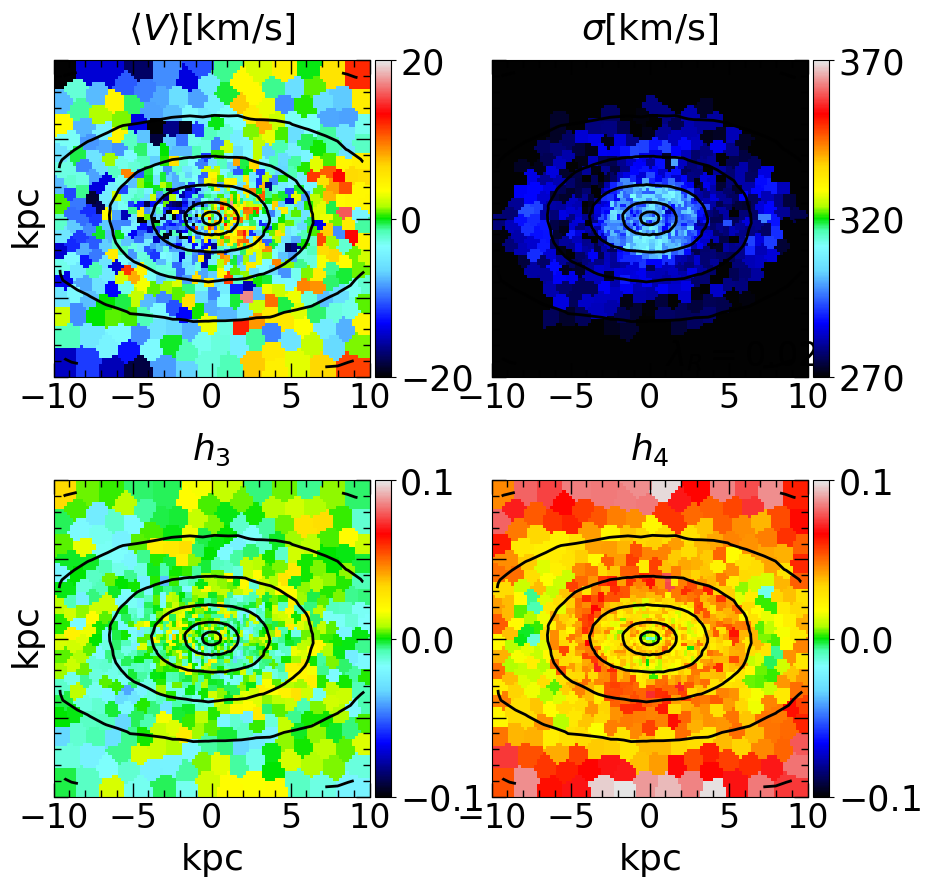
\includegraphics[width=\textwidth]{BH_1.png}
		\caption{BH-1 merger}
	\end{subfigure}
	\begin{subfigure}[b]{0.49\textwidth}
		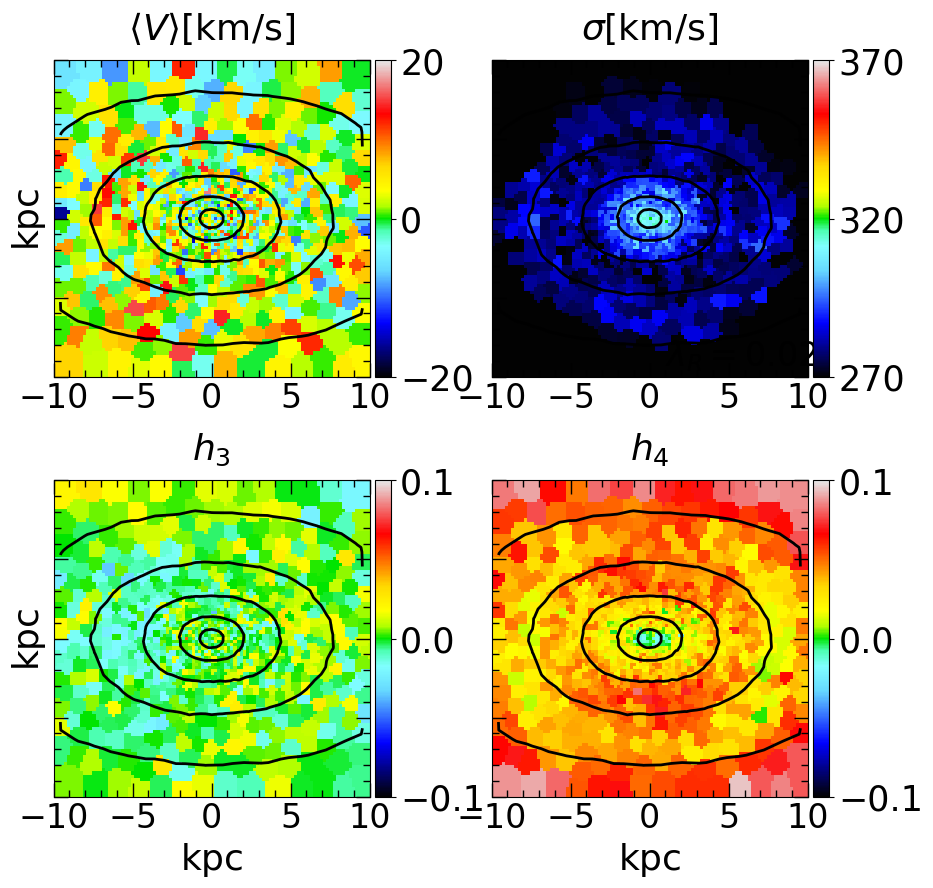
\includegraphics[width=\textwidth]{BH_2.png}
		\caption{BH-2 merger}
	\end{subfigure}
	\begin{subfigure}[b]{0.49\textwidth}
		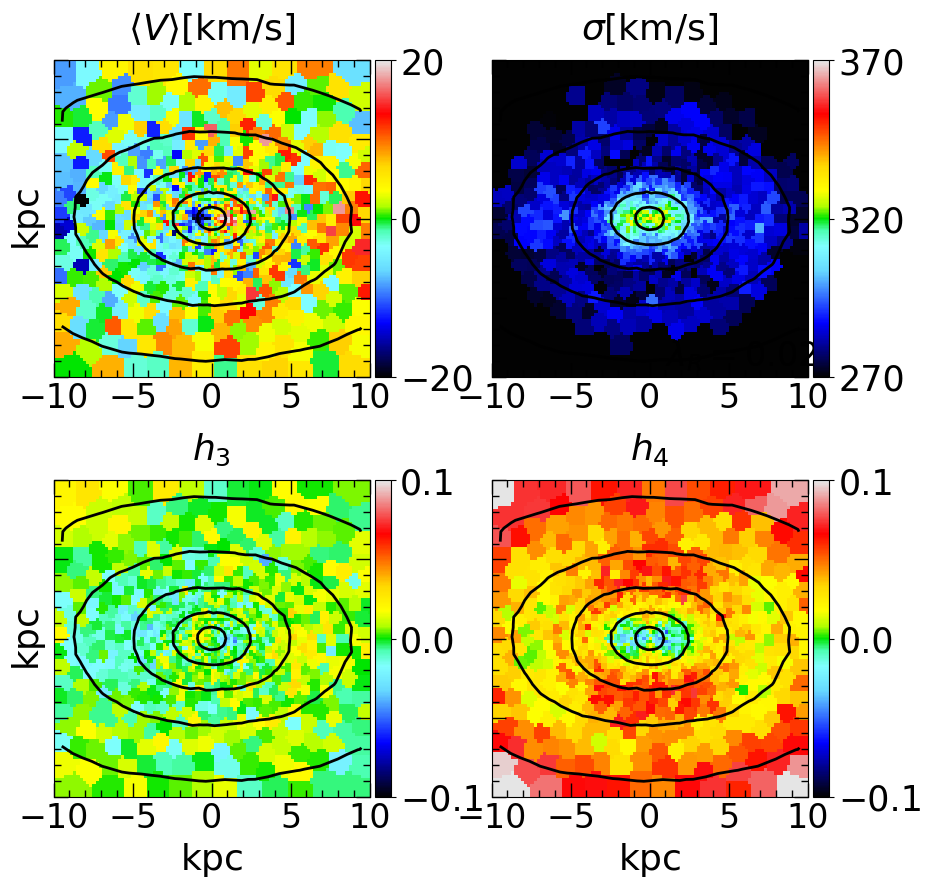
\includegraphics[width=\textwidth]{BH_3.png}
		\caption{BH-3 merger}
	\end{subfigure}
	\begin{subfigure}[b]{0.49\textwidth}
		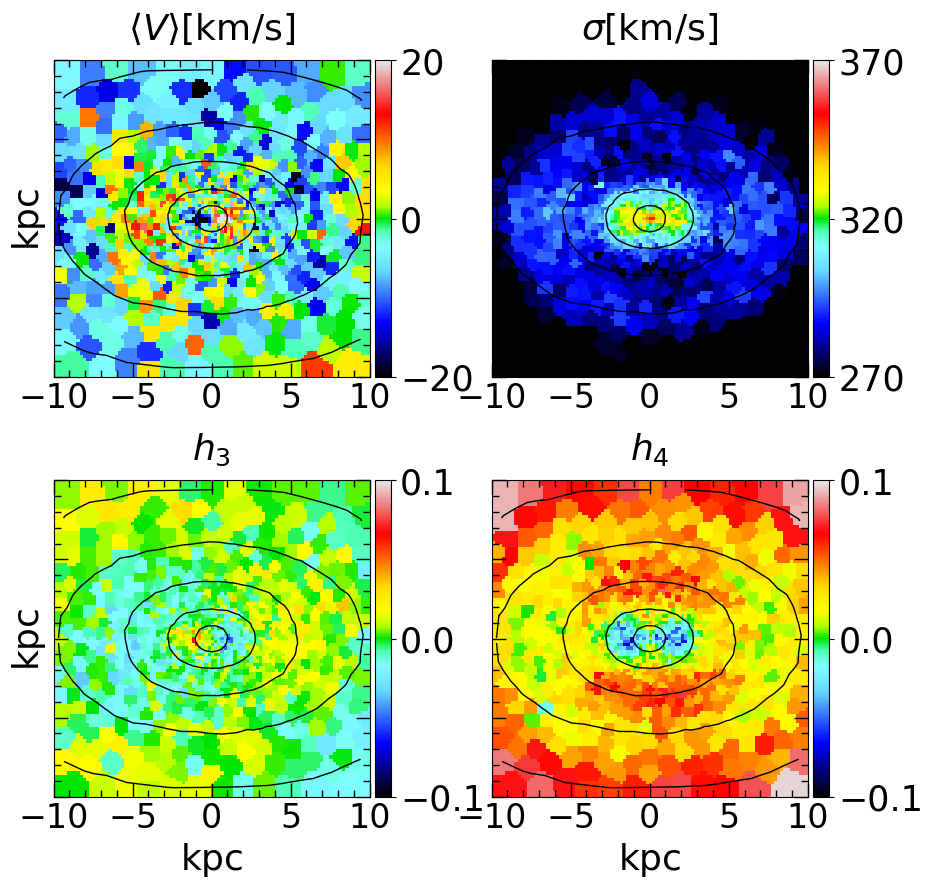
\includegraphics[width=\textwidth]{BH_4.png}
		\caption{BH-4 merger}
	\end{subfigure}
	\begin{subfigure}[b]{0.49\textwidth}
		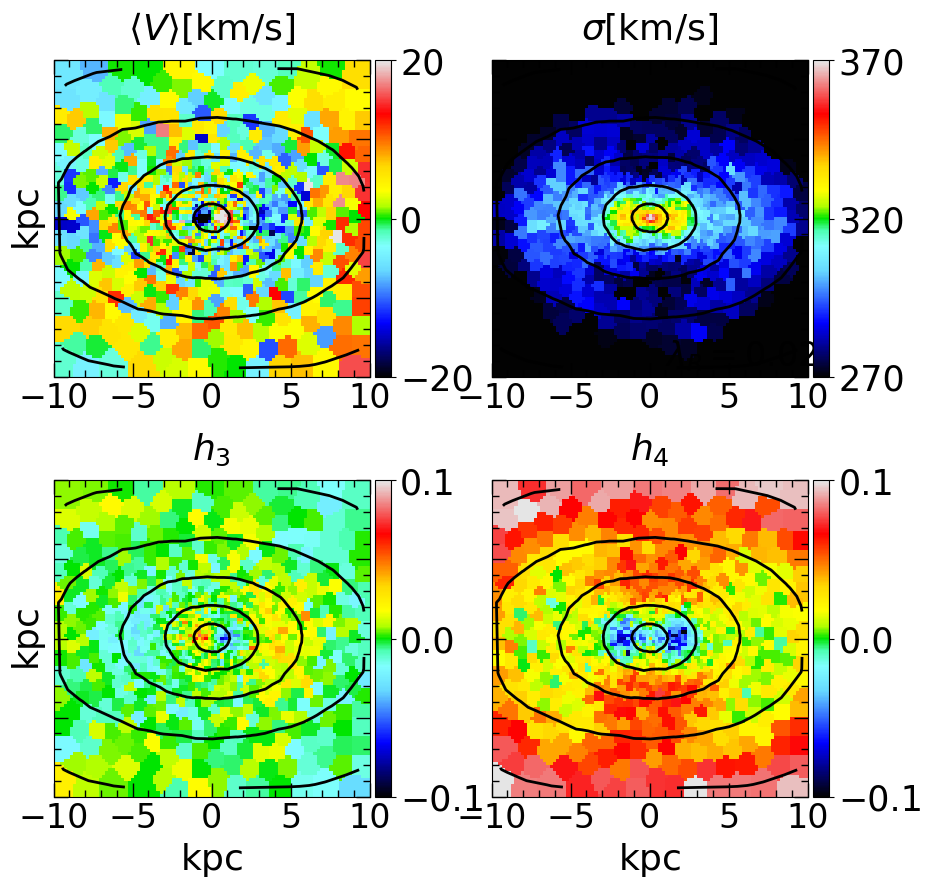
\includegraphics[width=\textwidth]{BH_5.png}
		\caption{BH-5 merger}
	\end{subfigure}
	\caption{IFU-maps of average LOS-velocities, velocity dispersion, $h_3$ parameters and $h_4$ parameters from four simulated merger remnants: BH-1, BH-2, BH-3, BH-4 and BH-5 mergers.}
	\label{figure:rest_of_voronoi}
\end{figure}


 %Furthermore, the velocity dispersion maps also show features found in observed galaxies (figure \ref{figure:IFU-maps}). \textit{Stuff about the features?}

Apart from the BH-0 merger remnant, the $h_3$-parameter values in the IFU-maps of the simulated merger remnants show an anti-correlation with the average LOS-velocity. Indeed, \cite{Krajnovic2011} have found that, while the anti-correlation between the LOS velocities and the $h_3$-parameter is mostly found in fast rotators (see central region of the fast-rotator NGC 4111 in figure \ref{figure:IFU-maps}), some galaxies with CRCs also exhibit this behaviour. Thus, this anti-correlation can be seen in for example the slowly rotating NGC 3414 in figure \ref{figure:IFU-maps}. Looking at the simulated merger remnants, this anti-correlation seems to be more pronounced in the remnants that contain a more massive the central SMBH binary. Furthermore, the larger binary mass seems to also make the counter-rotating central regions in the remnants clearer. Thus, there is a clear correlation between the degree of anti-correlation and the existence of CRCs in the simulated remnants, making the simulated KETJU results once again agree with observations.

The $h_4$-parameter roughly corresponds to the velocity anisotropy parameter $\beta$, where a negative value of $h_4$ identifies areas with a large tangential velocity dispersion, and a positive identifies areas with a more radial velocity dispersion \citep{Gerhard1993, Gerhard1998, Thomas2007}. Comparing the $\beta$-profiles from figure \ref{figure:beta_no_rb} with the $h_4$ IFU-maps from figures \ref{figure:IFU-maps} and \ref{figure:rest_of_voronoi}, this certainly seems to be the case. For the merger remnants with central SMBH binaries, both the $\beta$ and the $h_4$ values are largely positive in the outer regions of the galaxy, while being negative closer to their centres. The $h_4$ map of the BH-0 merger is then positive all around, exactly like its $\beta$-profile. The $h_4$ maps of NGC 3414 and NGC 4111 (figure \ref{figure:IFU-maps}) do not contain any specific structures and seem to be completely isotropic. As the negative $h_4$-areas in the IFU maps of the simulated merger remnants are likely caused by core scouring, and as neither of the observed galaxies are cored galaxies \citep{Lauer2007}, they have most likely not experienced such a process, making the lack of clear structures understandable.

\subsection{The $\lambda_R$-parameter}

Further analysis of the kinematics of the simulated merger remnants can be done by studying the $\lambda_R$ parameter (equation \ref{eq:general_lambdar}). Calculating the value of $\lambda_R$ at the effective radius ($\lambda_{Re}$) of a galaxy, allows one to determine whether it is a slow or a fast rotator. I use the Voronoi binned statistics from the IFU-maps to calculate $\lambda_{Re}$ for every simulated merger remnant, and compare them to the three slow rotator thresholds described in section \ref{section:slow_fast_rotators}:
 \begin{align}
\begin{split}
\lambda_{Re} &< 0.1, \\
\lambda_{Re} &< 0.31\sqrt{\epsilon_e},\\
\lambda_{Re} &< 0.08 + \epsilon_e/4,
\end{split}
\end{align}
where $\epsilon_e$ is the ellipticity of the remnant at the effective radius.

As two of the three slow rotator thresholds require us to know the ellipticity of the galaxy, I wrote a program in Python that calculates the ellipticities of the simulated merger remnants. These ellipticity calculations are done using a method described in \cite{Zemp2011}, which uses the shape tensor:
\begin{equation}
\mathbf{S} = \frac{\int_V \rho(\mathbf{r}) \omega(\mathbf{r}) \mathbf{r} \mathbf{r}^T \; dV }{\int_V \rho{\mathbf{r}} \; dV},
\end{equation}
where $\mathbf{r}$ is position from the galactic centre, $\rho(\mathbf{r})$ is the mass density, $V$ is the volume of an enclosed ellipsoid with the elliptical radius $r_\mathrm{ell}$, and where the weighting function $\omega(\mathbf{r}) = 1$. The eigenvalues of the shape tensor correspond to $a^2/3$, $b^2/3$ and $c^2/3$; where $a$, $b$ and $c$ are the semi-principal axes. The parameters $a$ and $b$ correspond to the semi-major and semi-minor axes, respectively, and can be used to calculate the ellipticity (equation \ref{eq:ellipticity}). 

Simply calculating the shape tensor and getting the correct eigenvalues is not possible, as the elliptical radius $r_\mathrm{ell}$ is defined, in part, using the axis ratios $a/b$ and $a/c$:
\begin{equation}
r_\mathrm{ell} = \sqrt{x_\mathrm{ell}^2 + \frac{y_\mathrm{ell}^2}{(b/a)^2} + \frac{z_\mathrm{ell}^2}{(c/a)^2}}.
\end{equation}
This means that the calculation has to be turned into an iterative process. Starting with $b/a = c/a = 1$ for the initial value of $r_\mathrm{ell}$, new shape tensor eigenvalues are calculated using previously gained axis ratios, until the values of the ratios start to converge. Once the difference between two subsequent axis ratios falls below some pre-defined convergence criterion, the newest $b/a$-ratio is used to calculate the ellipticity.

\begin{figure}
	\centering
	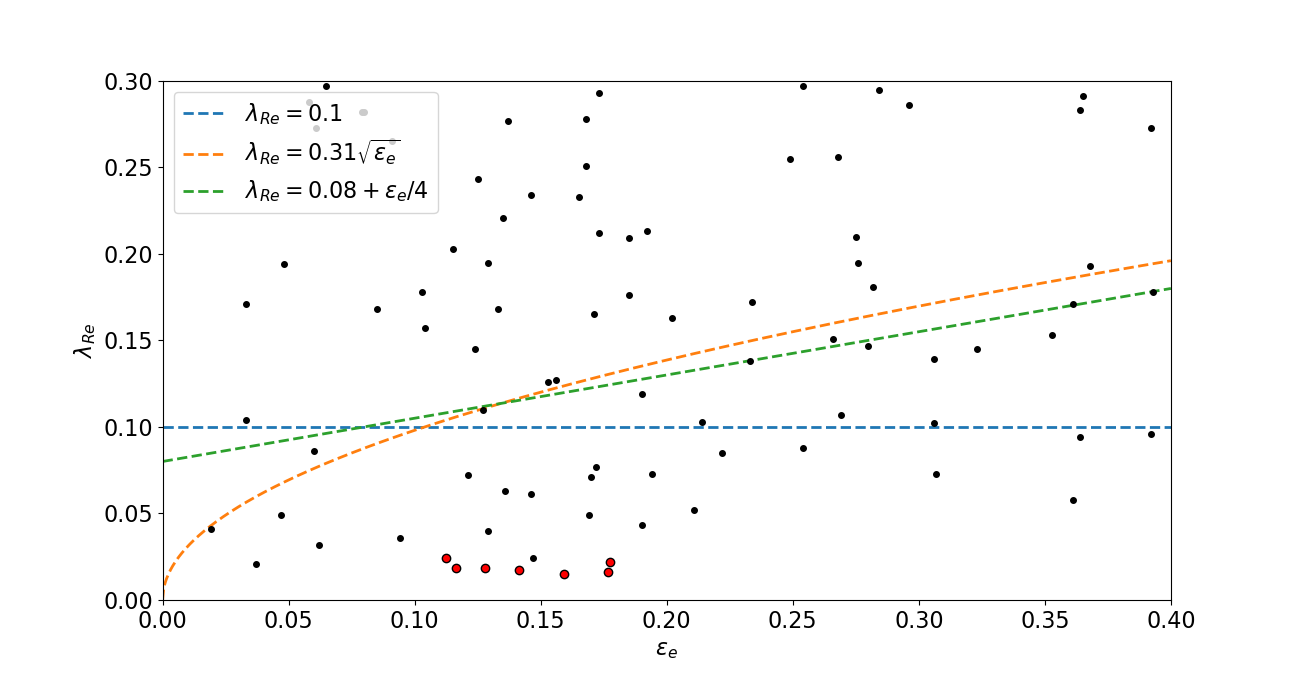
\includegraphics[width=\textwidth]{lambda_epsilon.png}
	\caption{Values of the $\lambda_{\mathrm{Re}}$-parameter of galaxies, plotted against their ellipticity at the effective radius. The red dots correspond to the simulated merger remnants, whereas the black dots correspond to galaxies observed in the $\mathrm{ATLAS^{3D}}$-survey \citep{Cappellari2011, Emsellem2011}. The dashed lines display different slow rotator thresholds as a function of ellipticity \citep{Emsellem2007, Emsellem2011, Cappellari2016}.}
	\label{figure:lambda_epsilon}
\end{figure}

Plotting $\lambda_{Re}$ and $\epsilon_e$ against each other (the ellipticity is calculated using $r_\mathrm{ell} = R_e$, and a convergence criterion of a difference smaller than $10^{-3}$ between consequent axis ratios), alongside the slow rotator thresholds and observed values from the $\mathrm{ATLAS^{3D}}$-survey \citep{Cappellari2011}, gives us figure \ref{figure:lambda_epsilon}. Regardless of the threshold used for differentiating between slow and fast rotators, the figure shows that, all of the simulated merger remnants are clearly classified as slow rotators. This agrees well with the kinematic anisotropies seen in the IFU-maps, which also implied a slow rotator classification for the remnants.

\section{Comparison to Observations}

As the physical properties of the merger progenitors are modelled after NGC 1600, it is interesting to see how the results from the simulations compare with actual observations of the galaxy. I will be comparing the observations mainly to the BH-6 merger remnant, as the mass of the SMBH binary in the simulated galaxy is equivalent to the observed and modelled mass of the central SMBH in NGC 1600 ($M_\bullet = 1.7 \times 10^{10} M_\odot$; \citealt{Thomas2016}). However, I will also be comparing the observed properties of the cored massive elliptical galaxy NGC 4472 to the simulated BH-1 merger remnant. Both of the latter galaxies have similar central black hole masses (or in the case of the simulated remnant, black hole binary mass), as well as similar total stellar masses. Thus, comparing their other physical properties could provide some interesting insight into the formation of cores.

Figure \ref{figure:profile_comparison} shows core-Sérsic profile fits of the surface brightness profiles from the BH-1 and BH-6 mergers, and compares them to the profile fits from the observed core galaxies NGC 4472 and NGC 1600, respectively. Not only do the shapes of the compared photometric profiles follow each other closely in both cases, the best-fit parameters are also quite closely related (table \ref{table:bestfit_parameter_comparison}). 

\begin{table}
	\begin{center}
		\scriptsize
		\begin{tabular}{| c | c c | c c |}
		\hline
		 & BH-1 merger & NGC 4472 & BH-6 merger & NGC 1600 \\
		\hline
		$r_b \; \mathrm{[kpc]}$ & $0.137$ & $0.151$ & $0.579$ & $0.667$ \\
		$\mu_b \; \mathrm{[mag \, arcsec^{-2}]}$ & $16.29$ & $16.48$ & $17.68$ & $18.00$ \\
		$R_e \; \mathrm{[kpc]}$ & $9.717$ & $16$ & $9.304$ & $16.04$ \\
		$n$ & $4$ & $5.6$ & $4$ & $5.83$ \\
		$\alpha$ & $1.45$ & $3.05$ & $1.22$ & $2.09$ \\
		$\gamma$ & $0.00$ & $0.06$ & $-0.04$ & $0.03$ \\
		\hline
		\end{tabular}
	\end{center}
	\caption{Best-fit parameters of the core-Sérsic profile fits seen in figure \ref{figure:profile_comparison}. The best-fit parameters of NGC 4472 are from \cite{Rusli2013}, while the parameters for NGC 1600 are given in \cite{Thomas2016}. $n$ is the Sérsic index, $\alpha$ controls the sharpness of the transition between the inner and outer profiles, and $\gamma$ is the slope of the inner profile.}
	\label{table:bestfit_parameter_comparison}
\end{table}

\begin{figure}
	\centering
	\begin{subfigure}[b]{0.49\textwidth}
		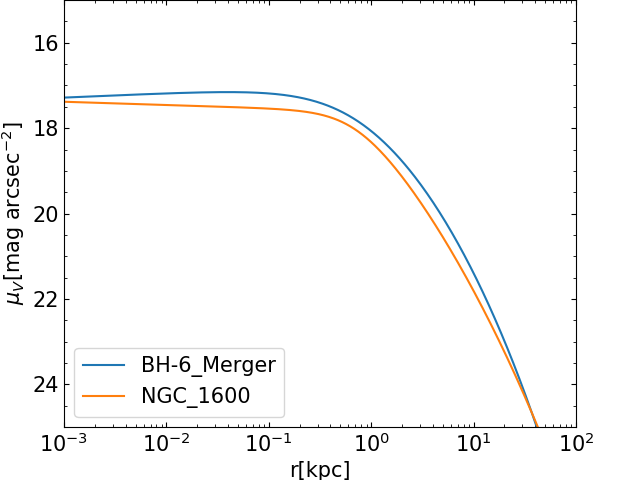
\includegraphics[width=\textwidth]{BH-6_NGC1600.png}
	\end{subfigure}
	\begin{subfigure}[b]{0.49\textwidth}
		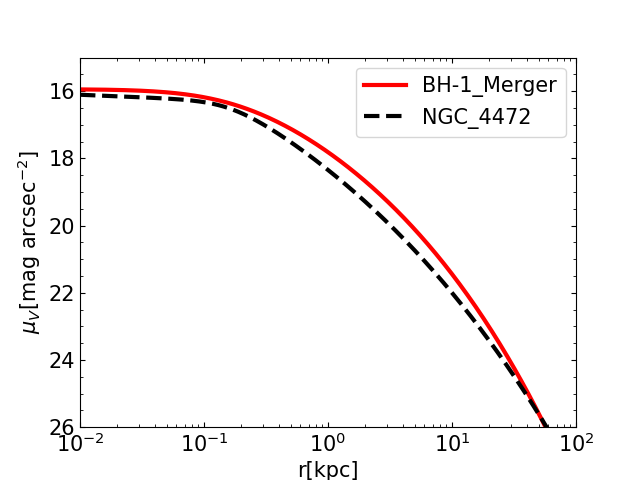
\includegraphics[width=\textwidth]{BH-1_NGC4472.png}
	\end{subfigure}
	\caption{Comparison between core-Sérsic profile fits from observed galaxies and simulated merger remnants. The surface brightness is given in V-band magnitudes. The figure on the left compares the profile of the BH-6 merger remnant to NGC 1600. The figure on the right compares the profiles of the BH-1 merger remnant  and NGC 4472. The parameters for plotting the core-Sérsic profile of NGC 1600 were taken from \cite{Thomas2016}, with their units being changed to the above by assuming that $V - R = 0.5$ (the same assumption being done in \cite{Lauer2007}), and by using the distance $D = 64 \mathrm{Mpc}$ \citep{Thomas2016} to define the relation between arc seconds and parsecs. The parameters for the profile of NGC 4472 were from \cite{Rusli2013}. All of the fitting parameters can be found in table \ref{table:bestfit_parameter_comparison}}
	\label{figure:profile_comparison}
\end{figure}

Another comparison between some of the properties of the four galaxies can be seen in table \ref{table:snap6_vs_NGC1600}. Most importantly, the table shows that the kinematic properties of the simulated merger remnants and the kinematic properties of NGC 1600 are very similar. On the other hand, compared to the three other galaxies, the $\lambda_e$-parameter and line-of-sight velocity of NGC 4472 are almost an order of magnitude larger. Furthermore, like the simulated galaxies, NGC 1600 can easily be identified as a slow rotator by its $\lambda_e$ parameter and ellipticity, while NGC 4472 seems to be classified as a fast rotator. 

Before drawing conclusion from these results, it is important to know that, whether NGC 4472 is in fact classified as a fast rotator is not known for certain. \cite{Emsellem2011} found a significantly lower value for its spin parameter ($\lambda_e = 0.077$), which would easily classify the object as a slow rotator. The value used in this analysis comes from the more recent MASSIVE-survey \citep{Ma2014MASSIVE, Veale2017veldisp}, in which some of the inaccuracies of the previous observations were shown (e.g. not taking into account a large enough region of the observed galaxy). Conceding to some potential biases in their own calculations, \cite{Veale2017veldisp} ultimately classify NGC 4472 as an intermediate case between slow and fast rotators.

It is impressive, that the simulation of the BH-6 merger is able to reproduce both the kinematic properties and the shape of the surface brightness profile of NGC 1600 so well. Since the simulation describes a dry major merger event between two massive ETG with central SMBHs, the results imply that this process could be the formation mechanism behind core galaxies. 

Interestingly, since the BH-1 merger has extremely similar kinematic properties with the BH-6 merger and NGC 1600, it can be assumed that the mass of the central SMBH binary does not affect the rotation of its host galaxy in any significant way. This suggests that, as far as the merger progenitors are concerned, it is the properties other than their central SMBH mass (i.e. them being massive gas-poor ETGs) that determine the stellar kinematics in the final merger remnant. As for NGC 4472, since both its $\lambda_e$ and LOS velocity are about an order of magnitude larger compared to the three other galaxies, it can be argued that its formation history must be quite different when compare to the other galaxies. However, due to the ambiguity of whether NGC 4472 is a fast rotator and whether its spin parameter is biased towards large values, the possibility that the galaxy has also formed through a dry ETG merger, should not be ruled out.

Earlier in this chapter it was shown that there is a clear positive correlation between the central SMBH binary masses and the size of the core radii in the simulated merger remnants. However, the facts that the core radius sizes for the BH-1 merger remnant and NGC 4472 are comparable and that many of their other properties are quite different, imply that, not only is there a correlation, the SMBH binary mass might be the only property that affects the size of the core in any significant way. If this is true, it is very strong evidence that the cores are formed through a scouring process by binary SMBHs.


\begin{table}
	\begin{center}
		\scriptsize
		\begin{tabular}{c c c c c c c c c c}
		\hline
		\hline
		Galaxy & $M_\star$ & $M_\bullet$ & $R_e$ & $\mu_e$ & $n$ & 
		$V_\mathrm{LOS}$ & $\sigma_e$ & $\lambda_e$ &
		$\epsilon_e$ \\
		& $[\times 10^{11} M_\odot]$ & $[\times 10^{10} M_\odot]$ &
		[kpc] & [$\mathrm{mag/arcsec^2}$] & & [km/s] & [km/s] & & \\
		(1) & (2) & (3) & (4) & (5) & (6) & (7) & (8) & (9) & (10) \\
		\hline
		BH-6 merger & $8.3$ & $1.7$ & $10.722$ & $21.54$ & $4$ & $5.61$ & $278$ & $0.0213$ & $0.15$ \\
		NGC 1600 & $8.3$ & $1.7$ & $\sim 16$ & $\sim 22.8$ & $5.83$ & $7.1$ & $293$ & $0.026$ & $0.32$ \\
		\hdashline
		BH-1 merger & $8.3$ & $0.17$ & $9.879$ & $21.42$ & $4$ & $5.49$ & $274$ & $0.021$ & $0.195$ \\
		NGC 4472 & $6.03$ & $0.25$ & $14.33$ & $22.72$ & $5.6$ & $45.4$ & 
		$258$ & $0.197$ & $0.172$ \\
		\hline
		\end{tabular}
	\end{center}
	\caption{Comparisons between the physical properties of the simulated BH-1 and BH-6 merger remnants, and the observed galaxies NGC 1600 and NGC 4472, respectively. The properties described in the columns are explained below, alongside the sources for their values in NGC 1600 and NGC 4472. \\
	(1) Name of the galaxy. \\
	(2) Total stellar mass. NGC 1600: \cite{Thomas2016}, NGC 4472: \cite{Veale2018lambda}. \\
	(3) Central SMBH / central SMBH binary mass. NGC 1600:  \cite{Thomas2016}, NGC 4472: \cite{Rusli2013_BHmass}. \\
	(4) Effective radius. The values used for the simulated mergers are estimated by calculating the half-mass radius in three dimensions, and using equation \ref{eq:projection_approximation} to get the approximate two dimensional effective radius. This is done instead of using the core-Sérsic profile best-fit parameter, since the core-Sérsic $R_e$ only takes into account the specific fitting radius. NGC 1600: \cite{Thomas2016}, where the value is changed from arc seconds to kpc by assuming that the galaxy is located at the distance of $D = 64 \; \mathrm{Mpc}$; NGC 4472: \cite{Veale2017veldisp}. \\
	(5) Surface brightness at the effective radius. The values for all of the galaxies are calculated from the core-Sérsic fits. \\
	(6) Sérsic index. NGC 1600: \cite{Thomas2016}, NGC 4472: \cite{Rusli2013}. \\
	(7) Mean line-of-sight velocity inside the effective radius. For the the simulated mergers these values are calculated from their respective IFU maps as the mean of the $V_\mathrm{LOS}$-values from the Voronoi-bins inside the effective radius. NGC 1600 and NGC 4472: \cite{Bender1994}. \\
	(8) Velocity dispersion inside the effective radius. As with $V_{LOS}$, this value comes from the mean velocity dispersion of the Voronoi bins inside the effective radius in the IFU-maps for the simulated mergers. NGC 1600 and NGC 4472: \cite{Veale2017veldisp}.\\
	(9) Spin parameter at the effective radius. NGC 1600 and NGC 4472: \citep{Veale2018lambda}. \\
	(10) For the simulated mergers and NGC 4472: ellipticity of the galaxy at the effective radius. For NGC 1600: luminosity weighted ellipticity. NGC 1600: \cite{Goullaud2018}, NGC 4472: \cite{Emsellem2011}.
	}
	\label{table:snap6_vs_NGC1600}
\end{table}


\chapter{Conclusions} \label{chapter:5}

In this Master's thesis, I have studied the formation of low-luminosity galactic cores in mergers of gas-free elliptical galaxies containing a central supermassive black hole. The central SMBHs are expected to form a coalescing binary during the merger, and I considered whether the cores form as a result of stellar material being ejected, due to strong gravitational interactions between the binary and its surrounding stars. I analysed the results from seven simulations describing such galaxy mergers (denoted as BH-0 - BH-6 mergers). The simulations were done using the KETJU code, a combination of both the GADGET-3 tree code \citep{Springel2005} and the AR-CHAIN integrator \citep{Mikkola2008ARCHAIN}, which can simulate both general galactic dynamics as well as precise stellar motion near SMBHs simultaneously. Each simulation run contained an almost identical galaxy merger, where only the masses of the central SMBHs changed from one simulation to another. The properties of the merger progenitor galaxies were modelled in such a way that, the resulting merger remnants should in principle resemble the known core galaxy NGC 1600.

The analysis of the simulation results, was mainly based on calculations of the surface brightness and velocity-anisotropy profiles of the simulated merger remnants, as well as their line-of-sight velocity distributions in the form of 2D Voronoi-binned kinematic maps. Additional quantities, such as the core radius and the $\lambda$-parameter, were then  derived from these properties. The results of the seven different simulations were compared with each other, alongside comparisons to observations of known core galaxies.

Analysing the surface brightness and velocity anisotropy profiles of the simulated merger remnants, I find them to strongly imply that the cores are, in fact, formed by SMBH mergers. Excluding two of the core radii derived using the Nuker-model, the core sizes determined from the surface brightness profiles, alongside with the amount of missing light in the centre of the profile, show a clear positive correlation with the SMBH binary mass. This is the most fundamental indication that the core formation is inherently linked to the central binary, as, assuming the binary merger hypothesis to be true, the larger binary mass would naturally result in the ejection of more stellar material due to its stronger gravitational influence. Furthermore, neglecting the clearly anomalous velocity anisotropy profile of the BH-2 merger, the $\beta$-profiles of the simulated remnants seem to also be affected as expected by changes in the mass of the central black hole binary, with more massive SMBHs resulting in steeper and more tangentially dominated central profiles. 

While I would consider the above to be clear evidence towards cores being formed by SMBH mergers, the small amount of questionable data outlined above, and why it does not affect the conclusions, warrants some discussion. Simply put, compared to the amount of results that corroborate the SMBH merger hypothesis, the anomalies are not substantial. Neither the abnormally large core radii, nor the divergent $\beta$-profile of the BH-2 merger, provide significant evidence for the existence of any systematic problems in the methods used for either of the analyses. Furthermore, in the case of the conflicting core radii, they have been calculated using the Nuker-profile fitting method, which has been shown to sometimes produce inconsistent results due its strong dependence on the fitting range. As for the abnormal $\beta$-profile of the BH-2 merger, it is hard to determine what causes its curious shape. Even when testing slightly different methods for calculating the velocity anisotropy profiles, its inconsistencies in relation to the other profiles remained constant. Although likely just a coincidence, the strangely featureless average LOS-velocity IFU-map of the BH-2 merger (figure \ref{figure:IFU-maps}), seems imply that, in the case of the BH-2 merger in particular, the inconsistencies might be caused by some issue in the velocity data itself.  

If the cores found in the simulated merger remnants are to be used as evidence for the SMBH merger hypothesis of core formation, the other properties of the remnant galaxies have to be consistent with observations of known core galaxies. Comparing the simulations to observations, I found this to in fact be the case. Through calculating the $\lambda$-parameter from their line-of-sight velocities, the simulated merger remnants can be unquestionably classified as slow rotator galaxies. Similarly, most observed core galaxies are also determined to be slow rotators. Furthermore, the 2D kinematic maps of the simulated remnants, show properties often seen in observed slow rotator galaxies, such as KDCs. The surface brightness profile of the BH-6 merger also has a close resemblance to the surface brightness profile of NGC 1600, the central SMBH of which has a mass corresponding to the central binary of the simulated merger. I would consider these similarities between the simulations and observations listed above, to corroborate the SMBH merger hypothesis.

There are some slight differences in the shape of the velocity anisotropy profile of NGC 1600, and the simulated remnant galaxies. The shape of the observed profile is somewhat steeper, when compared to the profiles of the simulated galaxies. This discrepancy can be, however, in part attributed to the fact that the simulations comprise of a single-generational merger, while the observed galaxy has been almost certainly formed gradually through multiple mergers. As such, the difference in the shape of the profile, does not contradict the SMBH merger core formation model. In fact, future research could try to reproduce these properties through simulations of multi-generational galaxy mergers. However, simply merging the previously simulated remnants with new progenitor galaxies is not reasonable, as the work-load of the simulation would grow significantly as the number of simulated particles increases. Using some bootstrap method to resample a smaller amount of particles according to the current phase space distribution of the remnant, could be used to mitigate this problem.

In general, future research on the effects that SMBHs have on galaxy formation, should likely concern itself with including gaseous components in the simulations. The addition of simulated gas would allow one to test some of the proposed solutions for discrepancies found in the simulation results of this thesis. For example, one could study whether the steeper central $\beta$-profile of NGC 1600 is caused by the adiabatic growth of the central SMBH. Moreover, the inclusion of gas would allow researchers to study the effects that SMBH mergers have during the formation of cusp galaxies in gas-rich mergers. It would be interesting to consider how the star-burst event, expected to occur in the mergers with high amounts of interstellar gas, affects the coalescence of the SMBH binary. Determining the effects that a potential SMBH merger has on the magnitude of the central high-luminosity cusp, could also provide further insight onto the formation history and internal structure of observed cusp galaxies.

The KETJU code is ideal for potentially simulating the effects of SMBHs on gas-rich galaxy mergers. Since it is built on top of GADGET-3, which is capable of simulating the motion of ideal gas through so-called "smoothed particle dynamics", KETJU naturally includes all of the routines that GADGET-3 uses to, not only calculate the dynamics of the gas, but also processes such as star formation and the radiative cooling. However, the version of KETJU used in this thesis, does not have the interactions between the SMBH particles and the GADGET-3 gas particles fully implemented. The gas cannot even be included in the AR-CHAIN regime. Further development of KETJU is thus necessary.

%Fortunately, the KETJU code is in active development, and is constantly being updated. The current version of the code still has room for improvement in terms of efficiency and precision. For example, in the regularised region of the integrator, interactions between particles that are close to each other but far away in the chain are calculated in centre-of-mass coordinates, and thus might contain significant round-off errors. This can be resolved through the use of structures like the "minimum-spanning-tree", which use a tree-like structure instead of a chain to store the smallest inter-particle distances. Since this allows for multiple of the smallest distances to be attributed to a single particle, it is ensured that the interactions between nearby particles are always calculated using the short "tree" distances.

%Studying sources that might initially seem abnormal, such as core galaxies, is essential for understanding the history and nature of the Universe. It allows us to test previously held theories about the formation of large scale structures, and thus test the current cosmological model itself. Whether the formation models of these structures conform to the current cosmological paradigm, provides either evidence for or against it. Since the merger simulations produce similar results to observations, I would argue that they support the hierarchical formation model for large-scale structures. Furthermore, the small deviations from observations seen in the results, can be explained to be the consequence of the simulations consisting of a single merger generation, further corroborating a $\Lambda \mathrm{CDM}$ cosmology for the Universe.

All in all, I must conclude that the thesis has been successful in its aims. Through analysing simulations of galaxy mergers, further evidence has been provided that the low-luminosity cores seen in some elliptical galaxies, are caused by the coalesce of binary SMBHs. It is clear that, efficient and precise simulation codes for large scale galactic dynamics like KETJU, are extremely effective for testing the formation models of observed structures. They allow researchers to follow the evolution of galaxies and other stellar systems, which would be impossible through purely observational means. Continuing to develop these codes is therefore fundamental for future research on the history of both the Universe and the complex systems that lie within.


% STEP 5:
% Uncomment the following lines and set your .bib file and desired bibliography style
% to make a bibliography with BibTeX.
% Alternatively you can use the thebibliography environment if you want to add all
% references by hand.


% Define journal names
\newcommand{\apj}{The Astrophysical Journal}
\newcommand{\mnras}{Monthly Notices of the Royal Astronomical Society}
\newcommand{\apjs}{The Astrophysical Journal Supplement}
\newcommand{\nat}{Nature}
\newcommand{\aj}{The Astronomical Journal}
\newcommand{\na}{New Astronomy}
\newcommand{\araa}{Annual Review of Astronomy and Astrophysics}
\newcommand{\aap}{Astronomy and Astrophysics}
\newcommand{\apjl}{The Astrophysical Journal Letters}
\newcommand{\prl}{Physical Review Letters}
\newcommand{\ssr}{Space Science Reviews}
\newcommand{\prd}{Physical Review D}
\newcommand{\pasp}{Publications of the Astronomical Society of the Pacific}
\newcommand{\zap}{Z. Astrophys.}

\clearpage
\addcontentsline{toc}{chapter}{Bibliography} % This lines adds the bibliography to the ToC
\bibliographystyle{apalike-oma}
\bibliography{bibliography.bib}


\end{document}

